% LaTeX-Vorlage für Abschlussarbeiten
% Lehrstuhl für Automatisierungstechnik/Informatik
% Bergische Universität Wuppertal
%
% ursprünglich erstellt von Nils Potthoff,
% 2020-2021 grundlegend überarbeitet von Simon Lohmann

%%%%%%%%%%%%%%%%%%%%%%%%%%%%%%%%%%%%%%%%%%%%%%%%%%%%%%%%%%%%%%%%%%%%%%%%%%%%%%%%
%%% Benutzer-Einstellungen %%%%%%%%%%%%%%%%%%%%%%%%%%%%%%%%%%%%%%%%%%%%%%%%%%%%%
%%%%%%%%%%%%%%%%%%%%%%%%%%%%%%%%%%%%%%%%%%%%%%%%%%%%%%%%%%%%%%%%%%%%%%%%%%%%%%%%
%%                                                                      %%%%%%%%
%      Einstellungen erfolgen in der Datei Einstellungen.tex             %%%%%%%
       %%%%%%%%%%%%%%%%%%%%%%%%%%%%%%%%%%%%%%%%%%%%%%%%%%%%%%%%%%%%%%%%%%%%%%%%%%%%%%%%
%%% DATEI-INFO %%%%%%%%%%%%%%%%%%%%%%%%%%%%%%%%%%%%%%%%%%%%%%%%%%%%%%%%%%%%%%%%%
%%%%%%%%%%%%%%%%%%%%%%%%%%%%%%%%%%%%%%%%%%%%%%%%%%%%%%%%%%%%%%%%%%%%%%%%%%%%%%%%
%%% In dieser Datei werden alle wichtigen Einstellungen der Vorlage gesetzt %%%%
%%% Hier darfst du Werte ändern ;-) %%%%%%%%%%%%%%%%%%%%%%%%%%%%%%%%%%%%%%%%%%%%
%%%%%%%%%%%%%%%%%%%%%%%%%%%%%%%%%%%%%%%%%%%%%%%%%%%%%%%%%%%%%%%%%%%%%%%%%%%%%%%%
%
%%%%%%%%%%%%%%%%%%%%%%%%%%%%%%%%%%%%%%%%%%%%%%%%%%%%%%%%%%%%%%%%%%%%%%%%%%%%%%%%
%%%%%%%%%%%%%%%%%%%%%%%%%%%%%%%%%%%%%%%%%%%%%%%%%%%%%%%%%%%%%%%%%%%%%%%%%%%%%%%%
\ifx\inPreamble\undefined \else %%%% 'MAGIC' %%%%%%%%%%%%%%%%%%%%%%%%%%%%%%%%%%%
%%%%%%%%%%%%%%%%%%%%%%%%%%%%%%%%%%%%%%%%%%%%%%%%%%%%%%%%%%%%%%%%%%%%%%%%%%%%%%%%
%%%%%%%%%%%%%%%%%%%%%%%%%%%%%%%%%%%%%%%%%%%%%%%%%%%%%%%%%%%%%%%%%%%%%%%%%%%%%%%%
%%%%%%% Pflicht-Einstellungen %%%%%%%%%%%%%%%%%%%%%%%%%%%%%%%%%%%%%%%%%%%%%%%%%%

\newcommand{\artderarbeit}{Bachelor-Thesis}
% Bachelor-Thesis, Master-Thesis

\newcommand{\thema}{So lautet das Thema der Thesis}
% Thema der Thesis (wie in der Aufgabenstellung)


\setbool{verlaengerung}{false}
% Gibt es eine Verlängerung der Bearbeitungszeit?
% Wenn ja, hier auf "true" setzen und die Datei Verlaengerung.pdf ersetzen

\setbool{danksagung}{false}
% Eine optionale Danksagung kann in der Datei "Danksagung.tex" formuliert werden


\newcommand{\autor}{Max Mustermann}
% Euer voller Name

\newcommand{\matrikelnummer}{1234567}
% Eure Matrikelnummer

\newcommand{\studiengang}{Informationstechnologie}
% Offizielle Bezeichnung des Studiengangs

\newcommand{\schwerpunkt}{Systems \& Components}
% Wenn es in Eurem Studiengang keine Schwerpunkte gibt einfach leer lassen



\newcommand{\lehrstuhl}{Lehrstuhl für Automatisierungstechnik/Informatik}
% Der Lehrstuhl, an dem die Thesis geschrieben wird

\newcommand{\betreuer}{Vorname Nachname M.Sc.}
% Betreuer? (falls mehrere: mit \\ trennen)

\newcommand{\prueferA}{Prof. Dr.-Ing. Vorname Nachname}
% Erstprüfer (siehe Anmeldung)

\newcommand{\prueferB}{Prof. Dr.-Ing. Vorname Nachname}
% Zweitprüfer (siehe Anmeldung)


\newcommand{\abgabedatum}{03. August 1972}
% Euer Abgabedatum

\newcommand{\ort}{Wuppertal}
% Ort

\newcommand{\schlagwoerter}{Thesis, Bachelor, Bergische Universität Wuppertal}
% Schlagwörter, mit denen man das PDF finden kann


%%% Ende der Pflicht-Einstellungen %%%%%%%%%%%%%%%%%%%%%%%%%%%%%%%%%%%%%%%%%%%%%
%%%%%%%%%%%%%%%%%%%%%%%%%%%%%%%%%%%%%%%%%%%%%%%%%%%%%%%%%%%%%%%%%%%%%%%%%%%%%%%%
%%%%%%%%%%%%%%%%%%%%%%%%%%%%%%%%%%%%%%%%%%%%%%%%%%%%%%%%%%%%%%%%%%%%%%%%%%%%%%%%
%%% Layout-Anpassung (Optional) %%%%%%%%%%%%%%%%%%%%%%%%%%%%%%%%%%%%%%%%%%%%%%%%

\setbool{doppelseitig}{true}			% Einseitiger oder doppelseitiger Druck?

\setbool{linksMarkieren}{true}			% Anklickbare Links im PDF-Dokument markieren?

\setbool{abbildungsverzeichnis}{true} 	% Abbildungsverzeichnis erzeugen?
\setbool{quellcodeverzeichnis}{true}	% Quellcodeverzeichnis erzeugen?
\setbool{tabellenverzeichnis}{true}		% Tabellenverzeichnis erzeugen?
\setbool{symbolverzeichnis}{true}		% Symbolverzeichnis erzeugen?
\setbool{akronymverzeichnis}{true}		% Akronymverzeichnis erzeugen?
\setbool{abkuerzungsverzeichnis}{true}	% Abkürzungsverzeichnis erzeugen?

\setbool{glossar}{true}					% Glossar erzeugen?

\setbool{verzeichnisseImInhaltsverzeichnis}{true} % Verzeichnisse im Inhaltsverzeichnis erwähnen?

\setbool{verzeichnisseZusammenfassen}{true} % Seitenumbruch zwischen den Verzeichnissen deaktivieren?

\setbool{zusatzErklaerung}{false} 		% Hiermit können zusätzliche Erklärungen eingebunden werden (wird im Normalfall nicht benötigt)


%%%%%%%%%%%%%%%%%%%%%%%%%%%%%%%%%%%%%%%%%%%%%%%%%%%%%%%%%%%%%%%%%%%%%%%%%%%%%%%%
%%% Farben (Optional) %%%%%%%%%%%%%%%%%%%%%%%%%%%%%%%%%%%%%%%%%%%%%%%%%%%%%%%%%%

\setbool{color}{true} % Farbe für Design-Elemente verwenden (true/false)

\newcommand{\colormodel}{cmyk} % z.B. cmyk, rgb oder gray
% Falls das Tool eurer Druckerei Schwarz-Weiß-Seiten trotz \setbool{color}{false}
% _fälschlicherweise_ als Farbseiten erkennt (das kann ziemlich teuer werden!), 
% könnt ihr hier das Farbmodell der Vorlage umstellen.
%
% So hatten wir schon einmal den Fall, dass eine Thesis-Druckerei die S/W-Seiten
% erst korrekt erkannt hat, wenn das (eigentlich für das Drucken ungeeignete)
% RGB-Modell verwendet wurde...
% 
% Bilder und eingebundene PDFs werden durch diese Einstellung nicht geändert!
%
% Ein paar Beispiele für sinnvolle Werte:
% {cmyk}  - CMYK (Cyan, Magenta, Yellow, Key) ist _das Farbmodell_ für alles was gedruckt wird.
%           Jede professionelle Druckerei kann damit umgehen!
%           => der Standard bei Drucksachen und daher auch in dieser Vorlage
%
% {rgb}   - RGB (Red, Green, Blue) ist ein Farbmodell für Bildschirme etc.
%           Im Gegensatz zum Druck mit Pigmenten (=subtraktive Farbmischung) wird
%           hier mit Licht gearbeitet (Additive Farbmischung). RGB ist daher nicht
%           für den Druck geeignet und wird vor dem Druckvorgang in ein anderes
%           Farbmodell (z.B. CMYK) umgewandelt.
%           => eigentlich falsch, wird in Einzelfällen aber von Druckereien angefordert
%
% {gray}  - Wer möchte, kann auch das Farbmodell "gray" verwenden. Dann werden alle
%           Farben direkt in Graustufen umgerechnet.
%           In diesem Fall wird zusätzlich \setbool{color}{false} empfohlen.
%           So wird die Darstellung von Quelltexten an die nun fehlenden Farben angepasst.
%
% Weblinks zum Thema:
% https://de.wikipedia.org/wiki/CMYK-Farbmodell
% https://de.wikipedia.org/wiki/RGB-Farbraum
% https://www.ctan.org/pkg/xcolor

%%%%%%%%%%%%%%%%%%%%%%%%%%%%%%%%%%%%%%%%%%%%%%%%%%%%%%%%%%%%%%%%%%%%%%%%%%%%%%%%
%%% Seitenränder %%%%%%%%%%%%%%%%%%%%%%%%%%%%%%%%%%%%%%%%%%%%%%%%%%%%%%%%%%%%%%%

\setlength{\bindekorrektur}{1.0cm}
% Wie breit ist der Teil, an dem die einzelnen Blätter 
% mit einander verklebt/anderweitig verbunden werden?

\setlength{\randAussen}{1.88cm} % 1.88 - 2.5cm (einseitig), 2.5 - 3.4cm (doppelseitig)
% Wie viel Rand außen neben dem Text (einseitig: wie viel Rand rechts neben dem Text)
% Innerer bzw. linker Rand wird daraus automatisch berechnet


%%%%%%%%%%%%%%%%%%%%%%%%%%%%%%%%%%%%%%%%%%%%%%%%%%%%%%%%%%%%%%%%%%%%%%%%%%%%%%%%
%%% Literatur-Anpassung (Optional) %%%%%%%%%%%%%%%%%%%%%%%%%%%%%%%%%%%%%%%%%%%%%
%
% Es gibt drei Arten von Quellen:
%
% Gruppe A : Quellen, die im Text mit \cite{...} zitiert wurden
% Gruppe B : Quellen, die mit \nocite{...} markiert wurden (und sonst nicht zitiert wurden)
% Gruppe C : Quellen, die gar nicht zitiert wurden

\setbool{nichtZitiertInweiterfuehrendeLiteratur}{true}
% nicht zitierte Quellen automatisch mit \nocite{} aufnehmen?
% => d.h. Gruppe C wird automatisch in Gruppe B verschoben 

\setbool{weiterfuehrendeLiteratur}{true}
% Separates Verzeichnis für weiterführende Literatur?
%
% "true": Separates Verzeichnis "Weiterführende Literatur" erstellen
%   Gruppe A => "Literatur"
%   Gruppe B => "Weiterführende Literatur"
% 
% "false": Alles landet in "Literatur"
%   Gruppe A => "Literatur"
%   Gruppe B => "Literatur"

\newcommand{\explizitesNocite}{
	% Wenn bei der Literatur Gruppe B manuell festgelegt werden soll, kann dies hier geschehen:
%	\nocite{ARM:AMBA4AXI4StreamProtocol:v1_0}
%	\nocite{ARM:AMBA_AXI_and_ACE_Protocol_Specification:E}
%	\nocite{AnalogDevices:ADAU1761:rev_C}
%	\nocite{Book:PerceptionBasedDataprocessingInAcoustics}
%	\nocite{Philips:I2S_BUS_Specification}
%	\nocite{Xilinx:PG021:v7_1}
%	\nocite{Xilinx:UG473:v1_11}
%	\nocite{Xilinx:UG761:v13_1}
%	\nocite{Xilinx:UG901:v2016_2}
%	\nocite{Xilinx:UG906:v2016_2}
%	\nocite{Xilinx:WP231}
%	\nocite{Xilinx:XAPP1206:v1_1}
%	\nocite{Xilinx:PG109:v9_0}
%	\nocite{ARM:NEONProgrammersGuide:v1_0}
%	\nocite{Book:TheScientistandEngineersGuidetoDigitalSignalProcessing}
%	\nocite{IEEE:754:2008}
%	\nocite{SpectrumAndSpectralDensityEstimationByTheDFTincludingAListOfWindowFunctions}
}

\setbool{alleAutorenExplizitNennen}{true} % Steuert die Nennung der Autoren im Literaturverzeichnis
% Hier gibt es zwei übliche Varianten:
% true  : Es werden immer alle Autoren genannt.
% false : Bis zu vier Autoren werden mit Namen genannt.
%           Gibt es mehr Autoren, werden die ersten drei genannt und
%           der Rest mit et al. abgekürzt (wie auch im Zitierschlüssel)

%%%%%%%%%%%%%%%%%%%%%%%%%%%%%%%%%%%%%%%%%%%%%%%%%%%%%%%%%%%%%%%%%%%%%%%%%%%%%%%%
%%% Sprach-Anpassung (Optional) %%%%%%%%%%%%%%%%%%%%%%%%%%%%%%%%%%%%%%%%%%%%%%%%
% Eine Liste der mögliche Sprachen finden sich in der Dokumentation zum LaTeX-Paket 'babel'
\newcommand{\hauptsprache}{ngerman} % Sprache, in der das Dokument geschrieben ist. Wird auch für die Verzeichnisnamen etc. verwendet
\newcommand{\weitereSprachen}{ngerman, english, french, latin}% weitere Sprachen, auf die kurzfristig mit \selectlanguage{language} gewechselt wird. (Wenn es mehrere sind werden diese mit Kommata getrennt)

%%%%%%%%%%%%%%%%%%%%%%%%%%%%%%%%%%%%%%%%%%%%%%%%%%%%%%%%%%%%%%%%%%%%%%%%%%%%%%%%
\fi %%%%%%%%%%%%%%%%%%%%%%%%%%%%%%%%%%%%%%%%%%%%%%%%%%%%%%%%%%%%%%%%%%%%%%%%%%%%
%%%%%%%%%%%%%%%%%%%%%%%%%%%%%%%%%%%%%%%%%%%%%%%%%%%%%%%%%%%%%%%%%%%%%%%%%%%%%%%%                                          %%%%%%
%                                                                        %%%%%%%
%%                                                                      %%%%%%%%
%%%%%%%%%%%%%%%%%%%%%%%%%%%%%%%%%%%%%%%%%%%%%%%%%%%%%%%%%%%%%%%%%%%%%%%%%%%%%%%%
%%%%%%%%%%%%%%%%%%%%%%%%%%%%%%%%%%%%%%%%%%%%%%%%%%%%%%%%%%%%%%%%%%%%%%%%%%%%%%%%
%%%%%%%%%%%%%%%%%%%%%%%%%%%%%%%%%%%%%%%%%%%%%%%%%%%%%%%%%%%%%%%%%%%%%%%%%%%%%%%%

%%%%%%%%%%%%%%%%%%%%%%%%%%%%%%%%%%%%%%%%%%%%%
%%% ! WARNUNG ! %%%%%%%%%%%%%%%%%%%%%%%%%%%%%
%%%%%%%%%%%%%%%%%%%%%%%%%%%%%%%%%%%%%%%%%%%%%
%%%  Diese Datei bitte nur bearbeiten,    %%%
%%%   wenn du ein LaTeX-Experte bist      %%%
%%%             U N D                     %%%
%%%  die Vorlage unbedingt ändern willst  %%%
%%%%%%%%%%%%%%%%%%%%%%%%%%%%%%%%%%%%%%%%%%%%%
%%%%%%%%%%%%%%%%%%%%%%%%%%%%%%%%%%%%%%%%%%%%%
%
%%%%%%%%%%%%%%%%%%%%%%%%%%%%%%%%%%%%%%%%%%%%%%%%%%%%%%%%%%%%%%%%%%%%%%%%%%%%%%%%
%%% DATEI-INFO %%%%%%%%%%%%%%%%%%%%%%%%%%%%%%%%%%%%%%%%%%%%%%%%%%%%%%%%%%%%%%%%%
%%%%%%%%%%%%%%%%%%%%%%%%%%%%%%%%%%%%%%%%%%%%%%%%%%%%%%%%%%%%%%%%%%%%%%%%%%%%%%%%
%%% Diese Datei richtet diverse Pakete und Befehle für die Vorlage ein %%%%%%%%%
%%%%%%%%%%%%%%%%%%%%%%%%%%%%%%%%%%%%%%%%%%%%%%%%%%%%%%%%%%%%%%%%%%%%%%%%%%%%%%%%
%
\def\inPreamble{}% Flag setzen: wird sind in der Präambel
%%%%%%%%%%%%%%%%%%%%%%%%%%%%%%%%%%%%%%%%%%%%%%%%%%%%%%%%%%%%%%%%%%%%%%%%%%%%%%%%
%%% Encoding %%%%%%%%%%%%%%%%%%%%%%%%%%%%%%%%%%%%%%%%%%%%%%%%%%%%%%%%%%%%%%%%%%%

\RequirePackage[utf8]{inputenc}
% UTF8 Codierte .tex-Dateien

\RequirePackage[T1]{fontenc}
% Benutzung der europäischen Schriftkodierung
% z.B. zur richtigen Darstellung von Umlauten


%%%%%%%%%%%%%%%%%%%%%%%%%%%%%%%%%%%%%%%%%%%%%%%%%%%%%%%%%%%%%%%%%%%%%%%%%%%%%%%%
%%% Werkzeuge %%%%%%%%%%%%%%%%%%%%%%%%%%%%%%%%%%%%%%%%%%%%%%%%%%%%%%%%%%%%%%%%%%

\RequirePackage{etoolbox}		% Einfacheres Programmieren in LaTeX
\RequirePackage{calculator}		% Rechnen (auch mit Längen)
\RequirePackage{xfp}			% Genaueres Rechnen (aber nicht mit Längen)
\RequirePackage{pbox}			% \pbox (Parbox flexibler Breite)


%%%%%%%%%%%%%%%%%%%%%%%%%%%%%%%%%%%%%%%%%%%%%%%%%%%%%%%%%%%%%%%%%%%%%%%%%%%%%%%%
%%% Variablen zur Anpassung durch den Benutzer %%%%%%%%%%%%%%%%%%%%%%%%%%%%%%%%%
%%%%%%%%%%%%%%%%%%%%%%%%%%%%%%%%%%%%%%%%%%%%%%%%%%%%%%%%%%%%%%%%%%%%%%%%%%%%%%%%
%%% >>> werden gesetzt in der Datei "PersoenlicheAngaben.tex" %%%%%%%%%%%%%%%%%%

\newbool{abbildungsverzeichnis}
\newbool{quellcodeverzeichnis}
\newbool{tabellenverzeichnis}
\newbool{symbolverzeichnis}
\newbool{akronymverzeichnis}
\newbool{abkuerzungsverzeichnis}
\newbool{glossar}

\newbool{verzeichnisseZusammenfassen}
\newbool{verzeichnisseImInhaltsverzeichnis}

\newbool{nichtZitiertInweiterfuehrendeLiteratur}
\newbool{weiterfuehrendeLiteratur}
\newbool{alleAutorenExplizitNennen}

\newbool{verlaengerung}
\newbool{danksagung}
\newbool{zusatzErklaerung}

\newbool{color}
\newbool{linksMarkieren}

\newbool{doppelseitig}

\newlength{\bindekorrektur}
\setlength{\bindekorrektur}{1cm}

\newlength{\randAussen}
\setlength{\randAussen}{1.88cm} % 1.88 - 2.5cm (einseitig), 2.5 - 3.4 cm (doppelseitig)


%%%%%%%%%%%%%%%%%%%%%%%%%%%%%%%%%%%%%%%%%%%%%%%%%%%%%%%%%%%%%%%%%%%%%%%%%%%%%%%%
%%% Benutzer-Einstellungen anwenden %%%%%%%%%%%%%%%%%%%%%%%%%%%%%%%%%%%%%%%%%%%%

%%%%%%%%%%%%%%%%%%%%%%%%%%%%%%%%%%%%%%%%%%%%%%%%%%%%%%%%%%%%%%%%%%%%%%%%%%%%%%%%
%%% DATEI-INFO %%%%%%%%%%%%%%%%%%%%%%%%%%%%%%%%%%%%%%%%%%%%%%%%%%%%%%%%%%%%%%%%%
%%%%%%%%%%%%%%%%%%%%%%%%%%%%%%%%%%%%%%%%%%%%%%%%%%%%%%%%%%%%%%%%%%%%%%%%%%%%%%%%
%%% In dieser Datei werden alle wichtigen Einstellungen der Vorlage gesetzt %%%%
%%% Hier darfst du Werte ändern ;-) %%%%%%%%%%%%%%%%%%%%%%%%%%%%%%%%%%%%%%%%%%%%
%%%%%%%%%%%%%%%%%%%%%%%%%%%%%%%%%%%%%%%%%%%%%%%%%%%%%%%%%%%%%%%%%%%%%%%%%%%%%%%%
%
%%%%%%%%%%%%%%%%%%%%%%%%%%%%%%%%%%%%%%%%%%%%%%%%%%%%%%%%%%%%%%%%%%%%%%%%%%%%%%%%
%%%%%%%%%%%%%%%%%%%%%%%%%%%%%%%%%%%%%%%%%%%%%%%%%%%%%%%%%%%%%%%%%%%%%%%%%%%%%%%%
\ifx\inPreamble\undefined \else %%%% 'MAGIC' %%%%%%%%%%%%%%%%%%%%%%%%%%%%%%%%%%%
%%%%%%%%%%%%%%%%%%%%%%%%%%%%%%%%%%%%%%%%%%%%%%%%%%%%%%%%%%%%%%%%%%%%%%%%%%%%%%%%
%%%%%%%%%%%%%%%%%%%%%%%%%%%%%%%%%%%%%%%%%%%%%%%%%%%%%%%%%%%%%%%%%%%%%%%%%%%%%%%%
%%%%%%% Pflicht-Einstellungen %%%%%%%%%%%%%%%%%%%%%%%%%%%%%%%%%%%%%%%%%%%%%%%%%%

\newcommand{\artderarbeit}{Bachelor-Thesis}
% Bachelor-Thesis, Master-Thesis

\newcommand{\thema}{So lautet das Thema der Thesis}
% Thema der Thesis (wie in der Aufgabenstellung)


\setbool{verlaengerung}{false}
% Gibt es eine Verlängerung der Bearbeitungszeit?
% Wenn ja, hier auf "true" setzen und die Datei Verlaengerung.pdf ersetzen

\setbool{danksagung}{false}
% Eine optionale Danksagung kann in der Datei "Danksagung.tex" formuliert werden


\newcommand{\autor}{Max Mustermann}
% Euer voller Name

\newcommand{\matrikelnummer}{1234567}
% Eure Matrikelnummer

\newcommand{\studiengang}{Informationstechnologie}
% Offizielle Bezeichnung des Studiengangs

\newcommand{\schwerpunkt}{Systems \& Components}
% Wenn es in Eurem Studiengang keine Schwerpunkte gibt einfach leer lassen



\newcommand{\lehrstuhl}{Lehrstuhl für Automatisierungstechnik/Informatik}
% Der Lehrstuhl, an dem die Thesis geschrieben wird

\newcommand{\betreuer}{Vorname Nachname M.Sc.}
% Betreuer? (falls mehrere: mit \\ trennen)

\newcommand{\prueferA}{Prof. Dr.-Ing. Vorname Nachname}
% Erstprüfer (siehe Anmeldung)

\newcommand{\prueferB}{Prof. Dr.-Ing. Vorname Nachname}
% Zweitprüfer (siehe Anmeldung)


\newcommand{\abgabedatum}{03. August 1972}
% Euer Abgabedatum

\newcommand{\ort}{Wuppertal}
% Ort

\newcommand{\schlagwoerter}{Thesis, Bachelor, Bergische Universität Wuppertal}
% Schlagwörter, mit denen man das PDF finden kann


%%% Ende der Pflicht-Einstellungen %%%%%%%%%%%%%%%%%%%%%%%%%%%%%%%%%%%%%%%%%%%%%
%%%%%%%%%%%%%%%%%%%%%%%%%%%%%%%%%%%%%%%%%%%%%%%%%%%%%%%%%%%%%%%%%%%%%%%%%%%%%%%%
%%%%%%%%%%%%%%%%%%%%%%%%%%%%%%%%%%%%%%%%%%%%%%%%%%%%%%%%%%%%%%%%%%%%%%%%%%%%%%%%
%%% Layout-Anpassung (Optional) %%%%%%%%%%%%%%%%%%%%%%%%%%%%%%%%%%%%%%%%%%%%%%%%

\setbool{doppelseitig}{true}			% Einseitiger oder doppelseitiger Druck?

\setbool{linksMarkieren}{true}			% Anklickbare Links im PDF-Dokument markieren?

\setbool{abbildungsverzeichnis}{true} 	% Abbildungsverzeichnis erzeugen?
\setbool{quellcodeverzeichnis}{true}	% Quellcodeverzeichnis erzeugen?
\setbool{tabellenverzeichnis}{true}		% Tabellenverzeichnis erzeugen?
\setbool{symbolverzeichnis}{true}		% Symbolverzeichnis erzeugen?
\setbool{akronymverzeichnis}{true}		% Akronymverzeichnis erzeugen?
\setbool{abkuerzungsverzeichnis}{true}	% Abkürzungsverzeichnis erzeugen?

\setbool{glossar}{true}					% Glossar erzeugen?

\setbool{verzeichnisseImInhaltsverzeichnis}{true} % Verzeichnisse im Inhaltsverzeichnis erwähnen?

\setbool{verzeichnisseZusammenfassen}{true} % Seitenumbruch zwischen den Verzeichnissen deaktivieren?

\setbool{zusatzErklaerung}{false} 		% Hiermit können zusätzliche Erklärungen eingebunden werden (wird im Normalfall nicht benötigt)


%%%%%%%%%%%%%%%%%%%%%%%%%%%%%%%%%%%%%%%%%%%%%%%%%%%%%%%%%%%%%%%%%%%%%%%%%%%%%%%%
%%% Farben (Optional) %%%%%%%%%%%%%%%%%%%%%%%%%%%%%%%%%%%%%%%%%%%%%%%%%%%%%%%%%%

\setbool{color}{true} % Farbe für Design-Elemente verwenden (true/false)

\newcommand{\colormodel}{cmyk} % z.B. cmyk, rgb oder gray
% Falls das Tool eurer Druckerei Schwarz-Weiß-Seiten trotz \setbool{color}{false}
% _fälschlicherweise_ als Farbseiten erkennt (das kann ziemlich teuer werden!), 
% könnt ihr hier das Farbmodell der Vorlage umstellen.
%
% So hatten wir schon einmal den Fall, dass eine Thesis-Druckerei die S/W-Seiten
% erst korrekt erkannt hat, wenn das (eigentlich für das Drucken ungeeignete)
% RGB-Modell verwendet wurde...
% 
% Bilder und eingebundene PDFs werden durch diese Einstellung nicht geändert!
%
% Ein paar Beispiele für sinnvolle Werte:
% {cmyk}  - CMYK (Cyan, Magenta, Yellow, Key) ist _das Farbmodell_ für alles was gedruckt wird.
%           Jede professionelle Druckerei kann damit umgehen!
%           => der Standard bei Drucksachen und daher auch in dieser Vorlage
%
% {rgb}   - RGB (Red, Green, Blue) ist ein Farbmodell für Bildschirme etc.
%           Im Gegensatz zum Druck mit Pigmenten (=subtraktive Farbmischung) wird
%           hier mit Licht gearbeitet (Additive Farbmischung). RGB ist daher nicht
%           für den Druck geeignet und wird vor dem Druckvorgang in ein anderes
%           Farbmodell (z.B. CMYK) umgewandelt.
%           => eigentlich falsch, wird in Einzelfällen aber von Druckereien angefordert
%
% {gray}  - Wer möchte, kann auch das Farbmodell "gray" verwenden. Dann werden alle
%           Farben direkt in Graustufen umgerechnet.
%           In diesem Fall wird zusätzlich \setbool{color}{false} empfohlen.
%           So wird die Darstellung von Quelltexten an die nun fehlenden Farben angepasst.
%
% Weblinks zum Thema:
% https://de.wikipedia.org/wiki/CMYK-Farbmodell
% https://de.wikipedia.org/wiki/RGB-Farbraum
% https://www.ctan.org/pkg/xcolor

%%%%%%%%%%%%%%%%%%%%%%%%%%%%%%%%%%%%%%%%%%%%%%%%%%%%%%%%%%%%%%%%%%%%%%%%%%%%%%%%
%%% Seitenränder %%%%%%%%%%%%%%%%%%%%%%%%%%%%%%%%%%%%%%%%%%%%%%%%%%%%%%%%%%%%%%%

\setlength{\bindekorrektur}{1.0cm}
% Wie breit ist der Teil, an dem die einzelnen Blätter 
% mit einander verklebt/anderweitig verbunden werden?

\setlength{\randAussen}{1.88cm} % 1.88 - 2.5cm (einseitig), 2.5 - 3.4cm (doppelseitig)
% Wie viel Rand außen neben dem Text (einseitig: wie viel Rand rechts neben dem Text)
% Innerer bzw. linker Rand wird daraus automatisch berechnet


%%%%%%%%%%%%%%%%%%%%%%%%%%%%%%%%%%%%%%%%%%%%%%%%%%%%%%%%%%%%%%%%%%%%%%%%%%%%%%%%
%%% Literatur-Anpassung (Optional) %%%%%%%%%%%%%%%%%%%%%%%%%%%%%%%%%%%%%%%%%%%%%
%
% Es gibt drei Arten von Quellen:
%
% Gruppe A : Quellen, die im Text mit \cite{...} zitiert wurden
% Gruppe B : Quellen, die mit \nocite{...} markiert wurden (und sonst nicht zitiert wurden)
% Gruppe C : Quellen, die gar nicht zitiert wurden

\setbool{nichtZitiertInweiterfuehrendeLiteratur}{true}
% nicht zitierte Quellen automatisch mit \nocite{} aufnehmen?
% => d.h. Gruppe C wird automatisch in Gruppe B verschoben 

\setbool{weiterfuehrendeLiteratur}{true}
% Separates Verzeichnis für weiterführende Literatur?
%
% "true": Separates Verzeichnis "Weiterführende Literatur" erstellen
%   Gruppe A => "Literatur"
%   Gruppe B => "Weiterführende Literatur"
% 
% "false": Alles landet in "Literatur"
%   Gruppe A => "Literatur"
%   Gruppe B => "Literatur"

\newcommand{\explizitesNocite}{
	% Wenn bei der Literatur Gruppe B manuell festgelegt werden soll, kann dies hier geschehen:
%	\nocite{ARM:AMBA4AXI4StreamProtocol:v1_0}
%	\nocite{ARM:AMBA_AXI_and_ACE_Protocol_Specification:E}
%	\nocite{AnalogDevices:ADAU1761:rev_C}
%	\nocite{Book:PerceptionBasedDataprocessingInAcoustics}
%	\nocite{Philips:I2S_BUS_Specification}
%	\nocite{Xilinx:PG021:v7_1}
%	\nocite{Xilinx:UG473:v1_11}
%	\nocite{Xilinx:UG761:v13_1}
%	\nocite{Xilinx:UG901:v2016_2}
%	\nocite{Xilinx:UG906:v2016_2}
%	\nocite{Xilinx:WP231}
%	\nocite{Xilinx:XAPP1206:v1_1}
%	\nocite{Xilinx:PG109:v9_0}
%	\nocite{ARM:NEONProgrammersGuide:v1_0}
%	\nocite{Book:TheScientistandEngineersGuidetoDigitalSignalProcessing}
%	\nocite{IEEE:754:2008}
%	\nocite{SpectrumAndSpectralDensityEstimationByTheDFTincludingAListOfWindowFunctions}
}

\setbool{alleAutorenExplizitNennen}{true} % Steuert die Nennung der Autoren im Literaturverzeichnis
% Hier gibt es zwei übliche Varianten:
% true  : Es werden immer alle Autoren genannt.
% false : Bis zu vier Autoren werden mit Namen genannt.
%           Gibt es mehr Autoren, werden die ersten drei genannt und
%           der Rest mit et al. abgekürzt (wie auch im Zitierschlüssel)

%%%%%%%%%%%%%%%%%%%%%%%%%%%%%%%%%%%%%%%%%%%%%%%%%%%%%%%%%%%%%%%%%%%%%%%%%%%%%%%%
%%% Sprach-Anpassung (Optional) %%%%%%%%%%%%%%%%%%%%%%%%%%%%%%%%%%%%%%%%%%%%%%%%
% Eine Liste der mögliche Sprachen finden sich in der Dokumentation zum LaTeX-Paket 'babel'
\newcommand{\hauptsprache}{ngerman} % Sprache, in der das Dokument geschrieben ist. Wird auch für die Verzeichnisnamen etc. verwendet
\newcommand{\weitereSprachen}{ngerman, english, french, latin}% weitere Sprachen, auf die kurzfristig mit \selectlanguage{language} gewechselt wird. (Wenn es mehrere sind werden diese mit Kommata getrennt)

%%%%%%%%%%%%%%%%%%%%%%%%%%%%%%%%%%%%%%%%%%%%%%%%%%%%%%%%%%%%%%%%%%%%%%%%%%%%%%%%
\fi %%%%%%%%%%%%%%%%%%%%%%%%%%%%%%%%%%%%%%%%%%%%%%%%%%%%%%%%%%%%%%%%%%%%%%%%%%%%
%%%%%%%%%%%%%%%%%%%%%%%%%%%%%%%%%%%%%%%%%%%%%%%%%%%%%%%%%%%%%%%%%%%%%%%%%%%%%%%%


%%%%%%%%%%%%%%%%%%%%%%%%%%%%%%%%%%%%%%%%%%%%%%%%%%%%%%%%%%%%%%%%%%%%%%%%%%%%%%%%
%%% Verzeichnis- & PDF-Verzeichnis-Einträge generieren %%%%%%%%%%%%%%%%%%%%%%%%%

%TODO Verwendung so anpassen, dass der Eintrag (=Linkziel) direkt beim entsprechenden Titel steht (=Titel auch mit \verzeichnisEintrag generieren und vom originalverzeichnis ausblenden?)
\newcommand{\verzeichnisEintrag}[2]{%
	% #1 Name
	% #2 Label (für PDF)
	\ifbool{verzeichnisseImInhaltsverzeichnis}{%
%		\ifbool{verzeichnisseZusammenfassen}{%
			%nichts
%		}{%
			\clearpage%
%		}%
		\phantomsection% damit die Seitenzahl auf jeden Fall stimmt
		\nopagebreak%
		\addcontentsline{toc}{chapter}{#1}% 
		\nopagebreak%
	}{%
		\pdfbookmark[0]{#1}{#2}% hier passte die Seitenzahl bisher immer, daher keine \phantomsection nötig
	}%
}


%%%%%%%%%%%%%%%%%%%%%%%%%%%%%%%%%%%%%%%%%%%%%%%%%%%%%%%%%%%%%%%%%%%%%%%%%%%%%%%%
%%% Document-Class %%%%%%%%%%%%%%%%%%%%%%%%%%%%%%%%%%%%%%%%%%%%%%%%%%%%%%%%%%%%%

\ifbool{doppelseitig}{
	\def\onetwoside{twoside}
}{
	\def\onetwoside{oneside}
}

\documentclass[
	\onetwoside,% twoside: zweiseitig, oneside: einseitig
	titlepage, 	% Titelseite steht für sich allein
	12pt,		% Schriftgröße
	a4paper, 	% A4-Papier
]{report}


%%%%%%%%%%%%%%%%%%%%%%%%%%%%%%%%%%%%%%%%%%%%%%%%%%%%%%%%%%%%%%%%%%%%%%%%%%%%%%%%
%%% Sprachen %%%%%%%%%%%%%%%%%%%%%%%%%%%%%%%%%%%%%%%%%%%%%%%%%%%%%%%%%%%%%%%%%%%

\RequirePackage[%
	main=\hauptsprache, %Umsetzung der deutschen Sprache nach neuer Rechtschreibung
	\hauptsprache, % muss hier nochmal erwähnt werden, damit \autoref das auch mitbekommt
	\weitereSprachen %Sprachen, die nur Abschnittsweise (z.B. für Zitate) verwendet werden
	]{babel}

\RequirePackage{translations}

\DeclareTranslation{German}{Bibliography}{Literatur}
\DeclareTranslation{English}{Bibliography}{Bibliography}
\DeclareTranslationFallback{Bibliography}{Bibliography}

\DeclareTranslation{German}{FurtherReading}{Weiterführende Literatur}
\DeclareTranslation{English}{FurtherReading}{Further Reading}
\DeclareTranslationFallback{FurtherReading}{Further Reading}

\DeclareTranslation{German}{abbreviationsname}{Abkürzungen}
\DeclareTranslation{English}{abbreviationsname}{Abbreviations}
\DeclareTranslationFallback{abbreviationsname}{Abbreviations}

%%%%%%%%%%%%%%%%%%%%%%%%%%%%%%%%%%%%%%%%%%%%%%%%%%%%%%%%%%%%%%%%%%%%%%%%%%%%%%%%
%%% Schriftarten, Schriftsatz %%%%%%%%%%%%%%%%%%%%%%%%%%%%%%%%%%%%%%%%%%%%%%%%%%

\RequirePackage{lmodern} % Schriftart lmodern nutzen
\RequirePackage{microtype} % Besserer Schriftsatz

%%%%%%%%%%%%%%%%%%%%%%%%%%%%%%%%%%%%%%%%%%%%%%%%%%%%%%%%%%%%%%%%%%%%%%%%%%%%%%%%
%%% Zitate, Anführungszeichen %%%%%%%%%%%%%%%%%%%%%%%%%%%%%%%%%%%%%%%%%%%%%%%%%%

\RequirePackage[
	autostyle, % Zitierstil an die aktuelle Sprache anpassen
	german=quotes, % wenn Deutsch -> „Anführungszeichen“ benutzen 
]{csquotes} %wird auch von biblatex verwendet

\renewcommand{\mkcitation}[1]{\,#1} % Umdefiniert um doppelklammerung bei \textquote+\cite zu verhindern

%%%%%%%%%%%%%%%%%%%%%%%%%%%%%%%%%%%%%%%%%%%%%%%%%%%%%%%%%%%%%%%%%%%%%%%%%%%%%%%%
%%% Literaturverwaltung %%%%%%%%%%%%%%%%%%%%%%%%%%%%%%%%%%%%%%%%%%%%%%%%%%%%%%%%
\def\autorenAnzahlImLiteraturverzeichnis{4}
\ifbool{alleAutorenExplizitNennen}{
	\def\autorenAnzahlImLiteraturverzeichnis{99}
}{}

\RequirePackage[backend=bibtex8,  %Daten von Bibtex holen
			style=alphabetic, %In der Form [Xil13] statt [1] referenzieren
			sorting=nyt,	      %Name,Year,Title 
			maxbibnames=\autorenAnzahlImLiteraturverzeichnis, %Anzahl maximal/minimal genannter Autoren im Literaturverzeichnis
			minbibnames=3, 
			maxcitenames=3, %Anzahl maximal/minimal genannter Autoren mit \citeauthor{...}
			mincitenames=3,
			maxsortnames=99, % Anzahl der Autoren, die in die Sortierung eingehen
			minsortnames=99,
			maxalphanames=4, % Maximale Anzahl Autoren, bei der jeder Autor mit einem Buchstaben in [ABCD] genannt wird
			minalphanames=3, % Anzahl Autoren, ab der [ABC+] verwendet wird
			]{biblatex}

\DeclareNameAlias{default}{family-given}% Format: Nachname, Vorname
\DefineBibliographyStrings{ngerman}{ 
	andothers = {{et\,al\adddot}}, % et al.
}
\renewcommand*{\multinamedelim}{\addsemicolon\space} % Zeichen zwischen den Autoren
%\renewcommand*{\finalnamedelim}{\addsemicolon\space} % Zeichen zwischen den letzten beiden Autoren

\addbibresource{Include/Literatur.bib} % Literatur-Datei laden

\DeclareBibliographyCategory{cited} % registrieren, welche Quellen zitiert wurden
\AtEveryCitekey{%
	\addtocategory{cited}{\thefield{entrykey}}%
}

\ifbool{nichtZitiertInweiterfuehrendeLiteratur}{
	\nocite{*} % alle nicht zitierten Quellen mit aufnehmen
}{
	\explizitesNocite
}


%%%%%%%%%%%%%%%%%%%%%%%%%%%%%%%%%%%%%%%%%%%%%%%%%%%%%%%%%%%%%%%%%%%%%%%%%%%%%%%%
%%% Seitengröße festlegen %%%%%%%%%%%%%%%%%%%%%%%%%%%%%%%%%%%%%%%%%%%%%%%%%%%%%%

% Berechnung der seitlichen Seitenränder:
\def\randAussenCm{}
\def\bindekorrekturCm{}
\LENGTHDIVIDE{\randAussen}{1cm}{\randAussenCm} 			% auf cm normieren
\LENGTHDIVIDE{\bindekorrektur}{1cm}{\bindekorrekturCm} 	% auf cm normieren

\newlength{\randRechtsAussen}	% Als Länge anlegen (bessere Wiederverwendbarkeit)
\newlength{\randLinksInnen}

\setlength{\randRechtsAussen}{\fpeval{1*\randAussenCm} cm}
\setlength{\randLinksInnen}{\fpeval{\randAussenCm/2+\bindekorrekturCm} cm}

% Anwenden
\usepackage[
%	showframe, 				% Seitenränder anzeigen - zum Debuggen
	layout=a4paper,			% Papierformat
	headheight=1.2cm,		% durch Kopfzeile festgelegt
	top=3.55cm,				% Abstand Text <-> oberer Seitenrand
	left=\randLinksInnen,	% Abstand Text <-> linker Seitenrand
	right=\randRechtsAussen,% Abstand Text <-> rechter Seitenrand
	bottom=3.7cm 			% Abstand Text <-> unterer Seitenrand
]{geometry}


%%%%%%%%%%%%%%%%%%%%%%%%%%%%%%%%%%%%%%%%%%%%%%%%%%%%%%%%%%%%%%%%%%%%%%%%%%%%%%%%
%%% (R), (C), TM (vor allem für Zitate und das Literaturverzeichnis) %%%%%%%%%%%

\newcommand{\markRegistered}[1]{#1$^\text{\tiny{\textregistered\xspace}}$}
\newcommand{\markCopyrighted}[1]{#1$^\text{\tiny{\copyright\xspace}}$}
\newcommand{\markTrademark}[1]{#1$^\text{\tiny{\texttrademark\xspace}}$}
\usepackage[official]{eurosym}


\usepackage{bbding}%Häkchen für abgehakte Dinge
\newcommand{\ok}{\Checkmark}
\newcommand{\x}{\XSolidBrush}
\newcommand{\xg}{\textcolor{gray}{\x}}


%%%%%%%%%%%%%%%%%%%%%%%%%%%%%%%%%%%%%%%%%%%%%%%%%%%%%%%%%%%%%%%%%%%%%%%%%%%%%%%%
%%% Farben %%%%%%%%%%%%%%%%%%%%%%%%%%%%%%%%%%%%%%%%%%%%%%%%%%%%%%%%%%%%%%%%%%%%%

\usepackage{xcolor}


% Universell nutzbar
\definecolor{Buw}			{cmyk}{0.55, 0.00, 1.00, 0.00} % Pantone 376
\definecolor{BuwEtikett}	{cmyk}{0.55, 0.00, 1.00, 0.10} % Pantone 376 + 10K

\definecolor{BuwFak01}		{cmyk}{0.08, 1.00, 0.65, 0.34} % Pantone 201
\definecolor{BuwFak02}		{cmyk}{1.00, 0.03, 0.34, 0.12} % Pantone 321
\definecolor{BuwFak03}		{cmyk}{1.00, 0.57, 0.12, 0.70} % Pantone 540
\definecolor{BuwFak04_oben}	{cmyk}{0.70, 0.30, 0.00, 0.12} % Pantone 646
\definecolor{BuwFak04_unten}{cmyk}{1.00, 0.61, 0.04, 0.26} % Pantone 301
\definecolor{BuwFak05}		{cmyk}{0.23, 0.17, 0.13, 0.46} % Pantone Cool Gray 8
\definecolor{BuwFak06_oben}	{cmyk}{0.37, 1.00, 0.00, 0.26} % Pantone 2425
\definecolor{BuwFak06_unten}{cmyk}{0.37, 1.00, 0.00, 0.47} % Pantone 2425 + 30K
\definecolor{BuwFak07}		{cmyk}{1.00, 0.00, 0.55, 0.40} % Pantone 562
\definecolor{BuwFak08}		{cmyk}{0.00, 0.00, 0.00, 0.00} %
\definecolor{BuwFak09}		{cmyk}{0.00, 0.30, 0.85, 0.00} % Pantone 1235

\definecolor{pureK}			{cmyk}{0.00, 0.00, 0.00, 1.00} % K

\definecolor{AccentStrong}	{cmyk}{0.000,0.420,0.800,0.100} % Orange
\definecolor{AccentWeak}	{cmyk}{0.295,0.142,0.000,0.310} % Bläuliches Grau

% Farbschema
\ifbool{color}{
	% wenn Farbe
	\colorlet{primaryTop}		{Buw}
	\colorlet{primaryMiddle}	{Buw}
	\colorlet{primaryBottom}	{Buw}
	\colorlet{secondaryTop}		{BuwFak06_oben}
	\colorlet{secondaryMiddle}	{BuwFak06_oben!50!BuwFak06_unten}
	\colorlet{secondaryBottom}	{BuwFak06_unten}
	\colorlet{tertiaryTop}		{black!50}
	\colorlet{tertiaryMiddle}	{black!50}
	\colorlet{tertiaryBottom}	{black!50}
	\colorlet{textBlack}		{black}
}{
	% wenn Graustufen
	\colorlet{primaryTop}		{pureK}
	\colorlet{primaryMiddle}	{pureK}
	\colorlet{primaryBottom}	{pureK}
	\colorlet{secondaryTop}		{pureK!70}
	\colorlet{secondaryMiddle}	{pureK!70}
	\colorlet{secondaryBottom}	{pureK!70}
	\colorlet{tertiaryTop}		{pureK!50}
	\colorlet{tertiaryMiddle}	{pureK!50}
	\colorlet{tertiaryBottom}	{pureK!50}
	\colorlet{textBlack}		{pureK}
}

% Kurzform für mittlere Farbe
\colorlet{primary}			{primaryMiddle}
\colorlet{secondary}		{secondaryMiddle}
\colorlet{tertiary}			{tertiaryMiddle}


% Spezialisierter Anwendungszweck
\colorlet{pagenumber}		{tertiaryBottom!50!textBlack}
\colorlet{headrule}			{primaryTop}
\colorlet{footnoteRule}		{secondary}
\colorlet{footrule}			{primaryBottom}

% TODO Formelnummern Style
\colorlet{captionLabel}		{pureK!80}
\colorlet{subcaptionLabel}	{pureK!70}

\colorlet{captionText}		{pureK!70}
\colorlet{subcaptionText}	{pureK!60}

\colorlet{listingBackground}{pureK!5}

%%%%%%%%%%%%%%%%%%%%%%%%%%%%%%%%%%%%%%%%%%%%%%%%%%%%%%%%%%%%%%%%%%%%%%%%%%%%%%%%
%%% Fußnotengestaltung %%%%%%%%%%%%%%%%%%%%%%%%%%%%%%%%%%%%%%%%%%%%%%%%%%%%%%%%%
%
\renewcommand{\footnoterule}{%
	\color{footnoteRule}{%
%	\textcolor{footnoteRule}{
% 	an der selben Stelle sorgt für Probleme mit umgebrochenen Listings.
%	Das liegt daran, dass \textcolor{}{} zusätzlich zu \color auch noch ein \leavevmode enthält.
%	Das \leavevmode wiederum bringt das Listing durcheinander, so dass z.B. die Zeilennummern direkt beim Umbruch 
%	jeweils vertauscht sind und oberhalb der untersten Zeile der vorderen Seite eine Lücke entsteht.
%	
		\vspace*{-3pt}%
		\hrule height 0.1em width 0.4\columnwidth%
		\vspace*{2.6pt}%
	}%
}%


%%%%%%%%%%%%%%%%%%%%%%%%%%%%%%%%%%%%%%%%%%%%%%%%%%%%%%%%%%%%%%%%%%%%%%%%%%%%%%%%
%%% Kopfzeilen und Fußzeilen, Seitenzahl %%%%%%%%%%%%%%%%%%%%%%%%%%%%%%%%%%%%%%%

\def\customFootrule{
	\renewcommand{\footrulewidth}{1.5mm}
	\renewcommand{\footrule}{%
		\begingroup
			\color{footrule}
			\hrule height \footrulewidth
			\vspace{0.5em}
		\endgroup
	}
}

\def\customHeadrule{
	\renewcommand{\headrulewidth}{1.5mm}
	\renewcommand{\headrule}{%
		\begingroup
			\color{headrule}
			\hrule height \headrulewidth 
		\endgroup
	}
}


\def\renewMarks{
	\renewcommand{\sectionmark}[1]{%
		\markright{%
			##1%~(\thesection)%
		}%
	}
	\renewcommand{\chaptermark}[1]{%
		\markboth{%
			##1% \chaptername~\thechapter%
		}{%
		}%
	}
}

\def\seitenNummer{%
	\color{pagenumber}\sffamily\bfseries\thepage{}%
}

\usepackage{fancyhdr} % Schönere Kopfzeilen
\def\vertikalZentrieren{%
	\vspace{-\footrulewidth}%
	\vspace{-1.275em}%
}

\ifbool{doppelseitig}{
	\def\rightodd{RO}
	\def\righteven{RE}
	\def\leftodd{LO}
	\def\lefteven{LE}
	\def\rightoddlefteven{RO,LE}
	\def\leftoddrighteven{LO,RE}
}{
	\def\rightodd{R}
	\def\righteven{R}
	\def\leftodd{R}
	\def\lefteven{R}
	\def\rightoddlefteven{R}
	\def\leftoddrighteven{L}
}

\fancypagestyle{thesis-page-regular}{%
	\renewMarks
	\fancyhf{}%clear
	\fancyhead[\rightoddlefteven]{%
		\includegraphics[height=2em]{\buwlogopdf}%
	}
	\fancyhead[\leftoddrighteven]{%
		\nouppercase{%
			\sffamily%
			\textbf{\leftmark}%
			\\%
			\rightmark%
		}%
	}
	\fancyfoot[\rightodd]{\vertikalZentrieren\colorbox{white}{\seitenNummer}\hspace{1em}}
	\fancyfoot[\lefteven]{\vertikalZentrieren\hspace{1em}\colorbox{white}{\seitenNummer}}
	
	\customHeadrule
	\customFootrule
}

\fancypagestyle{plain}{%
	\renewMarks
	\fancyhf{} % clear
	\fancyfoot[\rightodd]{\vertikalZentrieren\colorbox{white}{\seitenNummer}\hspace{1em}}
	\fancyfoot[\lefteven]{\vertikalZentrieren\hspace{1em}\colorbox{white}{\seitenNummer}}
	
	\customHeadrule
	\customFootrule
}


%%%%%%%%%%%%%%%%%%%%%%%%%%%%%%%%%%%%%%%%%%%%%%%%%%%%%%%%%%%%%%%%%%%%%%%%%%%%%%%%
%%% Format der Überschriften %%%%%%%%%%%%%%%%%%%%%%%%%%%%%%%%%%%%%%%%%%%%%%%%%%%

\usepackage[%
	nobottomtitles*,	% Überschriften am unteren Seitenrand vermeiden
]{titlesec}
 
\def\titleformatBase{\sffamily\bfseries}
\def\titleformatChapter{\Huge}
\def\titleformatSection{\LARGE}
\def\titleformatSubsection{\Large}
\def\titleformatSubsubsection{\large}
\def\titleformatParagraph{\normalsize}

\def\titlepartChapter	{\titleformatChapter\ifbool{weAreInTheAppendix}{\Alph{chapter}}{\arabic{chapter}}}
\def\titlepartSection	{\titleformatSection\arabic{section}}
\def\titlepartSubsection{\titleformatSubsection\arabic{subsection}}
\newbool{weAreInTheAppendix}
\setbool{weAreInTheAppendix}{false}
\appto{\appendix}{\setbool{weAreInTheAppendix}{true}}
\def\titleNumberExtraDistance{.5cm}

\titleformat{\chapter}[hang]
	{\titleformatBase}
	{\titlepartChapter\hphantom{.\titlepartSection.\titlepartSubsection}}
	{\titleNumberExtraDistance}
	{\titleformatChapter}
	%[after-code]
	
\titleformat{\section}[block]
	{\titleformatBase}
	{\color{textBlack!50}\titlepartChapter.\color{textBlack}\titlepartSection\hphantom{.\titlepartSubsection}}
	{\titleNumberExtraDistance}
	{\titleformatSection}
	%[after-code]

\titleformat{\subsection}[block]
	{\titleformatBase}
	{\color{textBlack!33}\titlepartChapter.\color{textBlack!50}\titlepartSection.\color{textBlack}\titlepartSubsection}
	{\titleNumberExtraDistance}
	{\titleformatSubsection}
	%[after-code]
	
\titleformat{\subsubsection}[block]
	{\titleformatBase}
	{\titleformatSubsubsection\thesubsubsection}
	{}
	{%
%	\hphantom{\titlepartChapter\titlepartSection\titlepartSubsection}\hspace{\titleNumberExtraDistance}%
	\titleformatSubsubsection}
	%[after-code]
	
\titleformat{\paragraph}[runin]
	{\titleformatBase}
	{\titleformatParagraph\theparagraph}
	{0em}
	{%
%	\hphantom{\titlepartChapter\titlepartSection\titlepartSubsection}\hspace{\titleNumberExtraDistance}%
	\titleformatParagraph}%
	[]
	%[after-code]
	
%				command			left	before	after
\titlespacing*{\chapter}		{0pt}	{-2.1em}{1em}
\titlespacing*{\section}		{0pt}	{1em}	{1em}
\titlespacing*{\subsection}		{0em}	{1em}	{1em}
\titlespacing*{\subsubsection}	{0em}	{1em}	{1em}
\titlespacing*{\paragraph}		{0em}	{1em}	{1em}

%%%%%%%%%%%%%%%%%%%%%%%%%%%%%%%%%%%%%%%%%%%%%%%%%%%%%%%%%%%%%%%%%%%%%%%%%%%%%%%%
%%% Grafiken %%%%%%%%%%%%%%%%%%%%%%%%%%%%%%%%%%%%%%%%%%%%%%%%%%%%%%%%%%%%%%%%%%%

\usepackage{graphicx}				% um Bilder einbinden zu können 
\usepackage{pdfpages}				% Ganzseitig externe PDFs einbinden (z.B. für Aufgabenstellung)

\usepackage{tikz}					% Zeichnen per Code


%%%%%%%%%%%%%%%%%%%%%%%%%%%%%%%%%%%%%%%%%%%%%%%%%%%%%%%%%%%%%%%%%%%%%%%%%%%%%%%%
%%% SI-Einheiten und Zahlendarstellung %%%%%%%%%%%%%%%%%%%%%%%%%%%%%%%%%%%%%%%%%

\usepackage[
	% Die Einstellungen für dieses Paket befinden sich in der Datei siunitx.cfg
]{siunitx}


%%%%%%%%%%%%%%%%%%%%%%%%%%%%%%%%%%%%%%%%%%%%%%%%%%%%%%%%%%%%%%%%%%%%%%%%%%%%%%%%
%%% Quellcode %%%%%%%%%%%%%%%%%%%%%%%%%%%%%%%%%%%%%%%%%%%%%%%%%%%%%%%%%%%%%%%%%%
\usepackage{listings} %Für Quelltexte

% manuell Übersetzen
\DeclareTranslation{German}{lstlistingname}{Quellcode}
\DeclareTranslation{English}{lstlistingname}{Sourcecode}
\DeclareTranslationFallback{lstlistingname}{\lstlistingname}
\renewcommand{\lstlistingname}{\GetTranslation{lstlistingname}}

\DeclareTranslation{German}{lstlistoflistingname}{Quellcodeverzeichnis}
\DeclareTranslation{English}{lstlistoflistingname}{List of Sourcecodes}
\DeclareTranslationFallback{lstlistoflistingname}{\lstlistlistingname}
\renewcommand{\lstlistlistingname}{\GetTranslation{lstlistoflistingname}}

\ifbool{color}{
	\def\listingBasicstyle		{\color{black}\ttfamily\small}
	\def\listingKeywordstyle	{\color{primary}\bfseries}
	\def\listingStringstyle		{\color{secondary}\slshape}
	\def\listingCommentstyle	{\color{AccentWeak}\fontseries{l}\selectfont}
	\def\listingEmphstyle		{\color{AccentStrong}\bfseries}
	\def\listingRulecolor		{\color{AccentWeak}}
	\def\listingNumbercolor		{\color{AccentWeak!60}}
}{
	\def\listingBasicstyle		{\color{pureK}\ttfamily\small}
	\def\listingKeywordstyle	{\color{pureK}\bfseries}
	\def\listingStringstyle		{\color{pureK}\slshape}
	\def\listingCommentstyle	{\color{pureK}\fontseries{l}\selectfont}
	\def\listingEmphstyle		{\color{pureK}\bfseries\underbar}
	\def\listingRulecolor		{\color{pureK!50}}
	\def\listingNumbercolor		{\color{pureK!26}}
}

\lstset{
	basicstyle	= \listingBasicstyle,		% Basisformat
	keywordstyle= \listingKeywordstyle,		% Schlüsselwörter
	stringstyle	= \listingStringstyle,		% Strings
	commentstyle= \listingCommentstyle,		% Kommentare
	emphstyle	= \listingEmphstyle,		% Hervorhebungen
%	
%	extendedchars=true,      	%Erweiterte Zeichensätze in Listings benutzen (aber nur Single-Byte!)   
	breaklines=true,            % Zeilen werden Umgebrochen
	breakatwhitespace=true,		% erlaube Zeilenumbrüche nur an Whitespace
	breakindent=0em,
	breakautoindent=true, % bei Zeilenumbruch automatisch einrücken
%
	prebreak=,
	postbreak=\mbox{$\hookrightarrow$\hspace{-0.34em}\hphantom{m}},
%	
	showstringspaces=true, 		% Leerzeichen in Strings zeigen
	showspaces=false,           % Leerzeichen anzeigen?
	showtabs=false,             % Tabs anzeigen?
	tabsize=3,					% Zeichenbreite eines Tabs
%	
	keepspaces=false,			% Erlaubt die Unterdrückung von Leerzeichen zugunsten eines besseren Spalten-Layouts
	columns=fixed,				% Zeichenbreite
%	
	captionpos=b, 				% Position der Beschriftung
	xleftmargin=2.2em, 			% Abstand zum Rand
	xrightmargin=0.35em,		%
	framexleftmargin=0em,		% Abstand im Rahmen
	framexrightmargin=0pt,		%
	framexbottommargin=2pt,		%
	framextopmargin=0pt,		%
	frame=tblr,					% Rahmen anzeigen
	frameround=tftf,			% t: abgerundete Ecke, f: eckige Ecke
	backgroundcolor=\color{listingBackground}, % Hintergrundfarbe
	rulecolor=\listingRulecolor,% Farbe der Umrandung
%
	numbers=left,
	numberstyle=\scriptsize\ttfamily\listingNumbercolor, %Stil der Zeilennummern
	stepnumber=1,
}

\lstset{literate= % Deutsche Umlaute und ß in Listings erlauben
	{Ö}{{\"O}}{1}
	{Ä}{{\"A}}{1}
	{Ü}{{\"U}}{1}
	{ß}{{\ss}}{1}
	%{ẞ}{{\MakeUppercase{\ss}}}{1} % KNOWNISSUE: der aktuell verwendete font enthält das zeichen leider nicht, also lieber erstmal weglassen ;-)
	{ü}{{\"u}}{1}
	{ä}{{\"a}}{1}
	{ö}{{\"o}}{1}
}
\linespread{1.25}
\lstdefinelanguage{thesis-latexbeispiel}
	{morekeywords=
		{\\begin, \\end, \\frac, \\pi, \\\\, \\sum, \\varphi, \\pm, \\int, \\limits, \\infty, \\cdot, \\sqrt, \\left, \\right, \\mathrm,
		\\linewidth, \\centering, \\includegraphics, \\caption, \\label, \\lstinline, \\lstinputlisting, \\todo, \\listoftodos, \\url, \\href, \\cite, \\textqoute,
		\\gls, \\glssymbol, \\LaTeX},
		emph={figure, table, tabular, align, lstlisting},
		sensitive=true,
		morecomment=[l]{\%},
%		morecomment=[s]{/*}{*/},
%		morestring=[b]",
		alsoletter={\\},
	}
	

%%%%%%%%%%%%%%%%%%%%%%%%%%%%%%%%%%%%%%%%%%%%%%%%%%%%%%%%%%%%%%%%%%%%%%%%%%%%%%%%
%%% Format der Float-Beschriftungen %%%%%%%%%%%%%%%%%%%%%%%%%%%%%%%%%%%%%%%%%%%%

\usepackage{caption}
\usepackage[labelformat=brace,list=true]{subcaption}
%Farbiger Text geht mit labelfont={bf,it,color=red}
% Mehr Infos zu CaptionStyle http://ctan.math.washington.edu/tex-archive/macros/latex/contrib/caption/caption-eng.pdf
\DeclareCaptionStyle{myCaptionStyle}{%
	format=plain,			% Basis-Format
	labelsep=quad,			% Abstand Typ/Nummer <-> Beschriftung
%	indention=-7em,			%
	margin=0.5em,				% Zusatzabstand Links
	singlelinecheck=false,	%
	labelfont={sf,small,bf,color=captionLabel},% Font Typ/Nummer
	textfont={sf,small, color=captionText},	% Font Beschriftung
%	justification=centering,
}

\DeclareCaptionStyle{mySubCaptionStyle}{%
	format=plain,			% Basis-Format
	labelsep=space,			% Abstand Typ/Nummer <-> Beschriftung
%	indention=-7em,			%
	margin=0.5em,			% Zusatzabstand links
	singlelinecheck=false,	%
	labelfont={sf,small,bf, color=subcaptionLabel},% Font Typ/Nummer
	textfont={sf,small, color=subcaptionText},	% Font Beschriftung
%	justification=centering,
}

% labelformat: empty  :
%              simple : a 
%              brace  : a)
%              parens : (a)


\captionsetup[table]{style=myCaptionStyle}
\captionsetup[figure]{style=myCaptionStyle}
\captionsetup[lstlisting]{style=myCaptionStyle}

\captionsetup[subfigure]{style=mySubCaptionStyle}
\captionsetup[subtable]{style=mySubCaptionStyle}


%%%%%%%%%%%%%%%%%%%%%%%%%%%%%%%%%%%%%%%%%%%%%%%%%%%%%%%%%%%%%%%%%%%%%%%%%%%%%%%%
%%% PDF-Meta-Informationen und Links im Dokument %%%%%%%%%%%%%%%%%%%%%%%%%%%%%%%

\usepackage[]{hyperref}

\ifbool{linksMarkieren}{
	% nichts
}{
	\hypersetup{hidelinks} % Link-Markierung verstecken
}

\hypersetup{
	linktoc=all, 						% Welcher Teil im Inhaltsverzeichnis ist klickbar? (none/section/page/all)
    colorlinks=false,					% false: boxed links (wird nicht mitgedruckt); true: colored links (wird auch so gedruckt!)
	linkcolor=primary!50!white,			% color of internal links
    linkbordercolor=primary!20!white,
%
    citecolor=primary!50!black,			% color of links to bibliography
    citebordercolor=primary!20!gray,
%
    filecolor=AccentStrong,				% color of file links
    filebordercolor=AccentStrong!20,
%
    urlcolor=AccentWeak,				% color of external links
    urlbordercolor=AccentWeak!20,
%
	menucolor=blue,
	menubordercolor=blue,
%
	runcolor=red,
	runbordercolor=red,
%
    %bookmarks=true,			% show bookmarks bar?
    unicode=true,				% non-Latin characters in Acrobat’s bookmarks
    pdftoolbar=true,			% show Acrobat’s toolbar?
    pdfmenubar=true,			% show Acrobat’s menu?
    pdffitwindow=false,			% window fit to page when opened
    pdfstartview={FitH},		% fits the width of the page to the window
    pdftitle=\thema,			% Titel
    pdfauthor=\autor,			% Autor
    pdfsubject=\artderarbeit,	% subject of the document
    pdfcreator=LaTeX,			% creator of the document
    pdfproducer=,				% producer of the document
    pdfkeywords=\schlagwoerter,	% Schlagworte
    pdfnewwindow=true,			% Links in neuem Fenster öffnen
}


%%%%%%%%%%%%%%%%%%%%%%%%%%%%%%%%%%%%%%%%%%%%%%%%%%%%%%%%%%%%%%%%%%%%%%%%%%%%%%%%
%%% Glossar, Abkürzungen, Akronyme, Symbole, ... %%%%%%%%%%%%%%%%%%%%%%%%%%%%%%%

\usepackage[
	toc=false,		% Nicht im Inhaltsverzeichnis anzeigen. Wenn die Verzeichnisse dort erscheinen sollen, machen wir das selber
	translate=babel,% Babel zum Übersetzen verwenden
	acronym,		% Eigenes Verzeichnis für Akronyme	(CRC, BAföG, LASER, ...)
	abbreviations,	% Eigenes Verzeichnis für Abkürzungen (Dr., z.B., bspw., bzw., etc.)
	symbols,		% Eigenes Verzeichnis für Symbole (µ, ...)
]{glossaries-extra}

\usepackage{glossary-longragged}% Extra Style
\usepackage{glossary-mcols}% Extra Style

% 'seename' wird mit translate=babel nicht übersetzt => dann machen wir das eben selber
\DeclareTranslation{German}{seename}{siehe}
\DeclareTranslation{English}{seename}{see}
\DeclareTranslationFallback{seename}{\seename} 
\renewcommand{\seename}{\expandonce{\GetTranslation{seename}}} %expandonce: es scheint so als würde der Befehl zu früh/spät expandiert - mit expandonce passt es


\makenoidxglossaries %langsames Sortieren, funktioniert aber immer und braucht keine externen Programme
\loadglsentries{Verzeichnisse/Glossar.tex}

%%%%%%%%%%%%%%%%%%%%%%%%%%%%%%%%%%%%%%%%%%%%%%%%%%%%%%%%%%%%%%%%%%%%%%%%%%%%%%%%
%%%%%%%%%%%%%%%%%%%%%%%%%%%%%%%%%%%%%%%%%%%%%%%%%%%%%%%%%%%%%%%%%%%%%%%%%%%%%%%%
% Anpassung von Nummerierungstiefe etc. (default passt aber schon)
%\setcounter{secnumdepth}{3} %Nummerierungstiefe
%\setcounter{tocdepth}{2} %Kapiteltiefe im Inhaltverzeichnis



\usepackage{blindtext}

%%%%%%%%%%%%%%%%%%%%%%%%%%%%%%%%%%%%%%%%%%%%%%%%%%%%%%%%%%%%%%%%%%%%%%%%%%%%%%%%
%%% Todos %%%%%%%%%%%%%%%%%%%%%%%%%%%%%%%%%%%%%%%%%%%%%%%%%%%%%%%%%%%%%%%%%%%%%%
\usepackage[
	ngerman,
%	textwidth=\randRechtsAussen-0em,%TODO sollte sich berechnen lassen, oder?
	textsize=scriptsize
]{todonotes}

\setlength{\marginparwidth}{\randAussen-2.5mm}% hieraus ergibt sich die Breite der Todo-Boxen


%%%%%%%%%%%%%%%%%%%%%%%%%%%%%%%%%%%%%%%%%%%%%%%%%%%%%%%%%%%%%%%%%%%%%%%%%%%%%%%%
%% Für Debugszwecke: Mehr Infos zu Boxen ausgeben:
%\showboxdepth=\maxdimen
%\showboxbreadth=\maxdimen







\usepackage{booktabs}
\usepackage{fancyvrb}
\newcommand{\VerbBar}{|}
\newcommand{\VERB}{\Verb[commandchars=\\\{\}]}
\DefineVerbatimEnvironment{Highlighting}{Verbatim}{commandchars=\\\{\}}



\DefineVerbatimEnvironment{Highlighting}{Verbatim}{commandchars=\\\{\}}
% Add ',fontsize=\small' for more characters per line
\newenvironment{Shaded}{}{}
\newcommand{\AlertTok}[1]{\textcolor[rgb]{1.00,0.00,0.00}{\textbf{#1}}}
\newcommand{\AnnotationTok}[1]{\textcolor[rgb]{0.38,0.63,0.69}{\textbf{\textit{#1}}}}
\newcommand{\AttributeTok}[1]{\textcolor[rgb]{0.49,0.56,0.16}{#1}}
\newcommand{\BaseNTok}[1]{\textcolor[rgb]{0.25,0.63,0.44}{#1}}
\newcommand{\BuiltInTok}[1]{#1}
\newcommand{\CharTok}[1]{\textcolor[rgb]{0.25,0.44,0.63}{#1}}
\newcommand{\CommentTok}[1]{\textcolor[rgb]{0.38,0.63,0.69}{\textit{#1}}}
\newcommand{\CommentVarTok}[1]{\textcolor[rgb]{0.38,0.63,0.69}{\textbf{\textit{#1}}}}
\newcommand{\ConstantTok}[1]{\textcolor[rgb]{0.53,0.00,0.00}{#1}}
\newcommand{\ControlFlowTok}[1]{\textcolor[rgb]{0.00,0.44,0.13}{\textbf{#1}}}
\newcommand{\DataTypeTok}[1]{\textcolor[rgb]{0.56,0.13,0.00}{#1}}
\newcommand{\DecValTok}[1]{\textcolor[rgb]{0.25,0.63,0.44}{#1}}
\newcommand{\DocumentationTok}[1]{\textcolor[rgb]{0.73,0.13,0.13}{\textit{#1}}}
\newcommand{\ErrorTok}[1]{\textcolor[rgb]{1.00,0.00,0.00}{\textbf{#1}}}
\newcommand{\ExtensionTok}[1]{#1}
\newcommand{\FloatTok}[1]{\textcolor[rgb]{0.25,0.63,0.44}{#1}}
\newcommand{\FunctionTok}[1]{\textcolor[rgb]{0.02,0.16,0.49}{#1}}
\newcommand{\ImportTok}[1]{#1}
\newcommand{\InformationTok}[1]{\textcolor[rgb]{0.38,0.63,0.69}{\textbf{\textit{#1}}}}
\newcommand{\KeywordTok}[1]{\textcolor[rgb]{0.00,0.44,0.13}{\textbf{#1}}}
\newcommand{\NormalTok}[1]{#1}
\newcommand{\OperatorTok}[1]{\textcolor[rgb]{0.40,0.40,0.40}{#1}}
\newcommand{\OtherTok}[1]{\textcolor[rgb]{0.00,0.44,0.13}{#1}}
\newcommand{\PreprocessorTok}[1]{\textcolor[rgb]{0.74,0.48,0.00}{#1}}
\newcommand{\RegionMarkerTok}[1]{#1}
\newcommand{\SpecialCharTok}[1]{\textcolor[rgb]{0.25,0.44,0.63}{#1}}
\newcommand{\SpecialStringTok}[1]{\textcolor[rgb]{0.73,0.40,0.53}{#1}}
\newcommand{\StringTok}[1]{\textcolor[rgb]{0.25,0.44,0.63}{#1}}
\newcommand{\VariableTok}[1]{\textcolor[rgb]{0.10,0.09,0.49}{#1}}
\newcommand{\VerbatimStringTok}[1]{\textcolor[rgb]{0.25,0.44,0.63}{#1}}
\newcommand{\WarningTok}[1]{\textcolor[rgb]{0.38,0.63,0.69}{\textbf{\textit{#1}}}} % Pakete und Kommandos (muss nicht geändert werden) %%
%%%%%%%%%%%%%%%%%%%%%%%%%%%%%%%%%%%%%%%%%%%%%%%%%%%%%%%%%%%%%%%%%%%%%%%%%%%%%%%%

% Selber eingebundene Pakete (optional)
%\usepackage{tikzducks} % Quack!

% Eigene Befehle & Definitionen (optional)
\newcommand{\zb}{z.\,B.}
\newcommand{\buw}{Bergische Universität Wuppertal}	  % Beispiel mit \newcommand
\newenvironment{vorlagenbeispiel}{\color{blue}}{}            % Beispiel-Umgebung

%%%%%%%%%%%%%%%%%%%%%%%%%%%%%%%%%%%%%%%%%%%%%%%%%%%%%%%%%%%%%%%%%%%%%%%%%%%%%%%%
\begin{document} % Hier beginnt das Dokument %%%%%%%%%%%%%%%%%%%%%%%%%%%%%%%%%%%
	
%%%%%%%%%%%%%%%%%%%%%%%%%%%%%%%%%%%%%%%%%%%%%
%%% ! WARNUNG ! %%%%%%%%%%%%%%%%%%%%%%%%%%%%%
%%%%%%%%%%%%%%%%%%%%%%%%%%%%%%%%%%%%%%%%%%%%%
%%%  Diese Datei bitte nur bearbeiten,    %%%
%%%   wenn du ein LaTeX-Experte bist      %%%
%%%             U N D                     %%%
%%%  die Vorlage unbedingt ändern willst  %%%
%%%%%%%%%%%%%%%%%%%%%%%%%%%%%%%%%%%%%%%%%%%%%
%%%%%%%%%%%%%%%%%%%%%%%%%%%%%%%%%%%%%%%%%%%%%
%
%%%%%%%%%%%%%%%%%%%%%%%%%%%%%%%%%%%%%%%%%%%%%%%%%%%%%%%%%%%%%%%%%%%%%%%%%%%%%%%%
%%% DATEI-INFO %%%%%%%%%%%%%%%%%%%%%%%%%%%%%%%%%%%%%%%%%%%%%%%%%%%%%%%%%%%%%%%%%
%%%%%%%%%%%%%%%%%%%%%%%%%%%%%%%%%%%%%%%%%%%%%%%%%%%%%%%%%%%%%%%%%%%%%%%%%%%%%%%%
%%% Diese Datei enthält die Titelseite und Standardteile am Anfang der Thesis %%
%%%%%%%%%%%%%%%%%%%%%%%%%%%%%%%%%%%%%%%%%%%%%%%%%%%%%%%%%%%%%%%%%%%%%%%%%%%%%%%%
%
\pagenumbering{Roman}
\pagestyle{plain}
%
% Entscheiden, welches der Logopdfs benutzt wird (verschiedene Schwarztöne)
\newcommand{\buwlogopdf}{Medien/Uni_Wuppertal_Logo__cmykblack.pdf}
\ifbool{color}{%
	\renewcommand{\buwlogopdf}{Medien/Uni_Wuppertal_Logo__richblack.pdf}
}{% color disabled
	\ifstrequal{\colormodel}{rgb}{%
		\renewcommand{\buwlogopdf}{Medien/Uni_Wuppertal_Logo__rgbblack.pdf}
	}{% cmyk/gray/...
		\renewcommand{\buwlogopdf}{Medien/Uni_Wuppertal_Logo__cmykblack}
	}
}
%
%%%%%%%%%%%%%%%%%%%%%%%%%%%%%%%%%%%%%%%%%%%%%%%%%%%%%%%%%%%%%%%%%%%%%%%%%%%%%%%%
%%% Titelseite %%%%%%%%%%%%%%%%%%%%%%%%%%%%%%%%%%%%%%%%%%%%%%%%%%%%%%%%%%%%%%%%%
%
	\begin{titlepage}
		\sffamily%
		%
		\hspace{-1.5em}%
		\includegraphics[width=4.5cm]{\buwlogopdf}%
		\hfill%
		\begin{minipage}[b]{\linewidth-4.5cm}
			\begin{flushright}
				\normalsize{Fakultät für Mathematik und Naturwissenschaften}%
				\vspace*{0.05mm}
			\end{flushright}
		\end{minipage}
		\vspace{-0.3em}
		\begingroup%
			\color{primary}%
			\rule{\textwidth}{3pt}%
		\endgroup%
		
		\vspace{3.2em}
		\begin{center}
			\textbf{\Huge{\artderarbeit}}%
			\vspace{1.4em}
			\\
			\textbf{\large{\thema}}%
		\end{center}
		
		
		\vfill
	
	
		\begin{center}
			\Large
			\autor%
			\\
			{\Large\matrikelnummer}%
			\bigskip\\%
			\studiengang%
			\\
			{\large\schwerpunkt}%
			\vspace{2em}%
			\hspace{0em}\\%
			\normalsize%
			\ort, den \abgabedatum%
		\end{center}
		
		
		\vspace{7.5em}
		
		
		\pbox[t][2em]{\linewidth}{Supervisor}%
		\quad%
		\pbox[t][2em]{\linewidth}{\betreuer}%
		\hfill%
		\pbox[t][2em]{\linewidth}{First Reviewer\\Second Reviewer}%
		\quad%
		\pbox[t][2em]{\linewidth}{\prueferA\\\prueferB}%
	
	\end{titlepage}
	\ifbool{doppelseitig}{%
		% im doppelseitigen Modus zählt report wie gewünscht
	}{%
		\stepcounter{page}% Seite manuell hochzählen, weil report das im einseitigen Modus nicht macht, im doppelseitigen aber schon (Konsistenz)
	}
	\clearpage{\pagestyle{empty}\cleardoublepage}
%
%
%%%%%%%%%%%%%%%%%%%%%%%%%%%%%%%%%%%%%%%%%%%%%%%%%%%%%%%%%%%%%%%%%%%%%%%%%%%%%%%%
%%% Themenblatt / Aufgabenstellung %%%%%%%%%%%%%%%%%%%%%%%%%%%%%%%%%%%%%%%%%%%%%
%
	% \pdfbookmark[1]{Aufgabenstellung}{aufgabe}%
	% 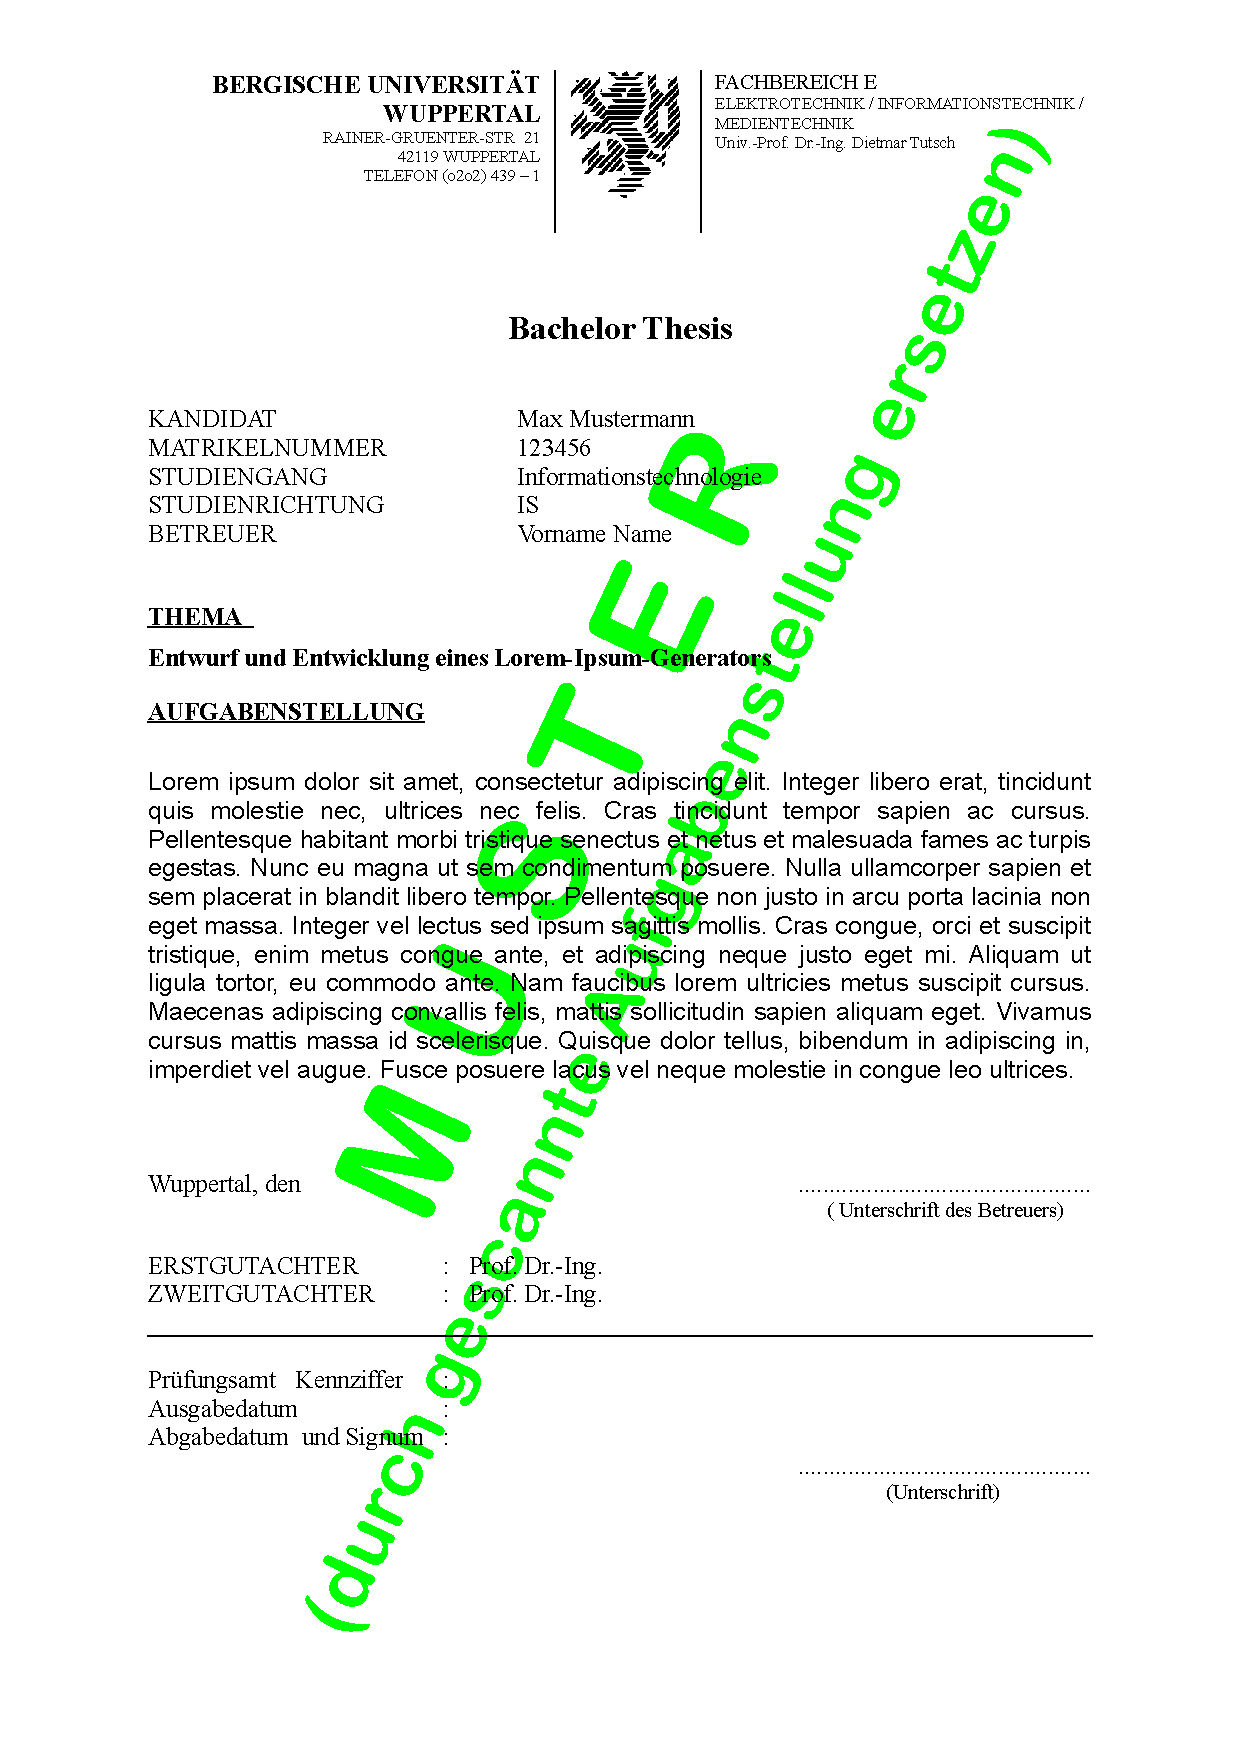
\includepdf[
	% 	pages={1},
	% 	fitpaper=true
	% ]{Medien/Aufgabenstellung.pdf}%
	% \clearpage{\pagestyle{empty}\cleardoublepage}%
%
%
%%%%%%%%%%%%%%%%%%%%%%%%%%%%%%%%%%%%%%%%%%%%%%%%%%%%%%%%%%%%%%%%%%%%%%%%%%%%%%%%
%%% Verlängerung %%%%%%%%%%%%%%%%%%%%%%%%%%%%%%%%%%%%%%%%%%%%%%%%%%%%%%%%%%%%%%%
%
	\ifbool{verlaengerung}{%
		\cleardoublepage%
		\pdfbookmark[1]{Verlängerung}{verlaengerung}%
		
\includepdf[pages={1},fitpaper=true]{Medien/Verlaengerung.pdf}%
	  	\clearpage{\pagestyle{empty}\cleardoublepage}%
	}{}%
%
%
%%%%%%%%%%%%%%%%%%%%%%%%%%%%%%%%%%%%%%%%%%%%%%%%%%%%%%%%%%%%%%%%%%%%%%%%%%%%%%%%
%%% Erklärungen %%%%%%%%%%%%%%%%%%%%%%%%%%%%%%%%%%%%%%%%%%%%%%%%%%%%%%%%%%%%%%%%
%
	\pdfbookmark[1]{Erklärungen}{erklaerung}%
	\vspace*{2em}%
	\section*{Eidesstattliche Erklärung}%
	\noindent Hiermit versichere ich, dass ich die Arbeit selbstständig verfasst, keine anderen als die angegebenen Quellen und Hilfsmittel benutzt sowie Zitate kenntlich gemacht habe.%
	
	\ifbool{zusatzErklaerung}{\vfill}{\vspace{4em}}%
	\begin{tabular}{lc}%
	\ort, den \abgabedatum \hspace*{1cm}& \rule[2px]{5cm}{0.5px}\\%
	                                    &\footnotesize{(Unterschrift)}%
	\end{tabular}
	\ifbool{zusatzErklaerung}{\vfill}{\vspace{5em}}%
	
	\section*{Einverständniserklärung}
	\noindent Ich bin damit einverstanden, dass meine Abschlussarbeit wissenschaftlich interessierten Personen oder Institutionen zur Verfügung gestellt werden kann. Korrektur- oder Bewertungshinweise in meiner Arbeit dürfen nicht zitiert werden.
	
	\ifbool{zusatzErklaerung}{\vfill}{\vspace{4em}}%
	\begin{tabular}{lc}
	\ort, den \abgabedatum \hspace*{1cm}& \rule[-2px]{5cm}{0.5px} \\ 
	                                       &\footnotesize{(Unterschrift)}
	\end{tabular}
	\ifbool{zusatzErklaerung}{%
		\vfill
		% Falls weitere Erklärungen gewünscht sind,
% können diese HIER eingefügt werden:
%
% Dies ist z.B. für den Fall gedacht, das eure Prüfungsordnung eine zusätzliche Erklärung einfordert...
%	
	\section*{Risikoaufklärung: \textit{Konsum von Text}} % Titel der Erklärung
	
	% Text der Erklärung:
	Dieses Beispiel enthält \emph{Text}. Der regelmäßige Konsum von hochkonzentriertem \emph{Text} kann unter Umständen Nebenwirkungen wie z.\,B. akuten Informationsgewinn, gesteigerte Redegewandheit oder verbesserten Satzbau zur Folge haben. Sofern Sie dies nicht beabsichtigen, hinterfragen Sie Ihre Motivation zu Studieren und/oder wenden Sie sich an eine entsprechende Beratungsstelle.
	\\
	
	
	{%
		\hrule
		\vspace{0.2em}
		\footnotesize%
		\sffamily%
		\noindent
		\textbf{Zu Risiken und Nebenwirkungen fragen Sie nicht Ihren Arzt oder Apotheker.}\\Dessen Wissen bezüglich Ihrer Thesisaktivitäten verhält sich zu Ihren Kentnissen I.d.R. orthogonal, d.h. es kann kein Zusammenhang hergeleitet werden. Der Erwartungswert der Verwirrtheit des Angesprochenen ergibt sich folglich aus dem reziproken Bekanntheitsgrad Ihrer Thesisaktivitäten reduziert um frühere Thesisaktivitäten des Angesprochenen.
		\hrule
	}~
	\\
	
	\noindent
	Ich habe die Risikoaufklärung zun möglichen Nebenwirkungen des Konsums von \emph{Text} gelesen\footnote{Gehen Sie weiter. Es gibt hier nichts zu sehen!} und akzeptiere die Möglichkeit eines ggf. unbeabsichtigten Wissensgewinns bei meiner Recherche.
	
	
	% Datum + Unterschrift-Feld (hier müsst Ihr normalerweise nichts ändern):
	\vfill
	\begin{tabular}{l c}
		\ort, den \abgabedatum \hspace*{1cm}& \rule[-2px]{5cm}{0.5px} \\ 
		&\footnotesize{(Unterschrift)}
	\end{tabular}
		\vfill
	}{}
	\clearpage	
%
%
%%%%%%%%%%%%%%%%%%%%%%%%%%%%%%%%%%%%%%%%%%%%%%%%%%%%%%%%%%%%%%%%%%%%%%%%%%%%%%%%
%%% Danksagung %%%%%%%%%%%%%%%%%%%%%%%%%%%%%%%%%%%%%%%%%%%%%%%%%%%%%%%%%%%%%%%%%
	\ifbool{danksagung}{%
		\vspace*{\fill}\vspace{-3em}%
		\pdfbookmark[1]{Danksagung}{danksagung}%
		\section*{Danksagung}
Text der Danksagung wird hier eingetragen.

Lorem ipsum dolor sit amet, consectetur adipiscing elit. Integer libero erat, tincidunt quis molestie nec, ultrices nec felis. Cras tincidunt tempor sapien ac cursus. Pellentesque habitant morbi tristique senectus et netus et malesuada fames ac turpis egestas. Nunc eu magna ut sem condimentum posuere. Nulla ullamcorper sapien et sem placerat in blandit libero tempor. Pellentesque non justo in arcu porta lacinia non eget massa. Integer vel lectus sed ipsum sagittis mollis. Cras congue, orci et suscipit tristique, enim metus congue ante, et adipiscing neque justo eget mi. Aliquam ut ligula tortor, eu commodo ante. Nam faucibus lorem ultricies metus suscipit cursus. Maecenas adipiscing convallis felis, mattis sollicitudin sapien aliquam eget. Vivamus cursus mattis massa id scelerisque. Quisque dolor tellus, bibendum in adipiscing in, imperdiet vel augue. Fusce posuere lacus vel neque molestie in congue leo ultrices.%
		\vfill%
	}{}
%
%
%%%%%%%%%%%%%%%%%%%%%%%%%%%%%%%%%%%%%%%%%%%%%%%%%%%%%%%%%%%%%%%%%%%%%%%%%%%%%%%%
%%% Kurzfassung & Abstract %%%%%%%%%%%%%%%%%%%%%%%%%%%%%%%%%%%%%%%%%%%%%%%%%%%%%
%
	\clearpage{\pagestyle{empty}\cleardoublepage}
	\vspace*{\fill}\vspace{-3em}
	\pdfbookmark[1]{Kurzfassung}{kurzfassung}
	% Kurzfassung auf Deutsch
\section*{Kurzfassung}

Entwicklerinnen und Entwickler stehen mit der Aufgabe gegenüber, eine große Menge an Informationen in ihrem Kurzzeitgedächtnis zu behalten, 
um den Code effektiv zu navigieren sowie dazu fähig zu sein, präzise Codeänderungen vorzunehmen, die sich gut in dem vorhandenen Code einfügen lassen.
Softwareentwicklerinnen und -entwickler müssen jedoch oft eine Vielzahl von verschiedenen Tools verwenden und in kurzen Abständen zwischen ihnen wechseln. Dies verursacht eine Unterbrechung 
die ihre Produktivität beeinträchtigt. 



Im Rahmen dieser Bachelorarbeit wird das Tool VSWorkbench entwickelt, um Entwicklerinnen und Entwickler bei ihren täglichen Aufgaben zu unterstützen.
VSWorkbench basiert auf Web-Technologien wie HTML, CSS und Javascript und legt den Fokus darauf, die Reibung in der Umgebung von Entwicklerinnen und Entwicklern zu verringern 
indem die Dauer solcher Unterbrechungen verkürzt werden. Zwei zentrale Softwareentwicklungstools, Visual Studio Code und GitLab, werden hierfür zusammengefuhrt 
 um den Durchsatz von Softwareentwicklerinnen und -entwicklern zu erhöhen. 

Die im Rahmen dieser Bachelorarbeit geleistete Arbeit ist auf Erweiterbarkeit ausgelegt und soll die Grundlage für die zukünftige Integration weiterer Plattformen legen.
Darüber hinaus wurden Schritte unternommen, um die künftige Zusammenarbeit mit der Open-Source Community zu erleichtern, z. B. durch das Open-Sourcing des Projekts auf GitHub.

\begingroup
	\selectlanguage{english}% einmal kurz auf englischen Textsatz wechseln
	
	\section*{Abstract}
    Developers often need to keep a big amount of information in their short time memory in order to navigate code effectively and be able to introduce precise code
    changes that integrate well with the already existing code.
    However; software developers' often need to use a diverse set of scattered tools, switching between them at small intervals. This causes an interruption 
    that is detrimental to their productivity. 

    

Within the frameowork of this bachlor's thesis, the VSWorkbench tool is developed to assist developers in their day to day tasks.
Built on web technologies such as HTML CSS and Javascript, VSWorkbench is a tool that aims to shrink friction in the environment of developers 
and shorten the length of such interruptions by bringing two central software development tools, 
Visual Studio Code and GitLab, closer together as a means of increasing the throughput of software developers. 

Built to be extensible, the work done within the framework of this bachelor's thesis should lay the basis for future integration of more platforms.
Moreover, steps were taken to facilitate future collaboration of the open source community, such as open sourcing the project on GitHub.
\endgroup


	\vfill
	\clearpage
%
%
%%%%%%%%%%%%%%%%%%%%%%%%%%%%%%%%%%%%%%%%%%%%%%%%%%%%%%%%%%%%%
%  INHALTSVERZEICHNIS
\markboth{\contentsname}{}
\pdfbookmark[1]{\contentsname}{toc}
\begingroup
	\renewcommand{\markboth}[2]{}{}
	\tableofcontents
\endgroup
\clearpage
%
%
%%WIDMUNG, VORWORT
%
%\nomenclature{$x$}{Description}
%\nomenclature{TEXT}{Abkürz}
%% Ende der Titelei; es folgt der Hauptteil
\ifbool{doppelseitig}{%
	\clearpage%
	\hphantom{anker, damit hier auch wirklich eine leere Seite ist}%
}{}%
{\pagestyle{empty}\cleardoublepage}% Inhalt soll auf rechter Seite beginnen
\pagenumbering{arabic}%
\pagestyle{thesis-page-regular}% % Titelseite etc. (bitte nicht ändern) %%%%%%%%%
	%%%%%%%%%%%%%%%%%%%%%%%%%%%%%%%%%%%%%%%%%%%%%%%%%%%%%%%%%%%%%%%%%%%%%%%%%%%%
	%%%%%%%%%%%%%%%%%%%%%%%%%%%%%%%%%%%%%%%%%%%%%%%%%%%%%%%%%%%%%%%%%%%%%%%%%%%%
	%%%%%%%%%%%%%  Ab hier ändern und ergänzen  %%%%%%%%%%%%%%%%%%%%%%%%%%%%%%%%
	%%%%%%%%%%%%%                               %%%%%%%%%%%%%%%%%%%%%%%%%%%%%%%%
	%%%%%%%%%%%%%  | | | | | | | | | | | | | |  %%%%%%%%%%%%%%%%%%%%%%%%%%%%%%%%   
	%%%%%%%%%%%%%  V V V V V V V V V V V V V V  %%%%%%%%%%%%%%%%%%%%%%%%%%%%%%%%
	% weitere .tex-Dateien werden mit \input eingebunden
	% (z.B. eine für jedes Kapitel)

	
	% Einführungskapitel
	\chapter{Einleitung}
	\section{Motivation}
		% Hier soll das Thema motiviert werden.
		% Bitte nicht "Ich bin besonders motiviert, weil ..."
		% sondern "Thema XY ist wichtig/muss untersucht/soll entwickelt werden, weil ..." 
		Thesisbeispiele sind super wichtig für ...
		
		
	\section{Problemstellung \& Ziele}
		% Hier sollen die Problemstellung und das Ziel der Thesis kurz in eigenen Worte erläutert werden.
		\blindtext
		
		
	\section{Aufbau der Thesis}
		% Überblick über den Aufbau der Thesis. Welche Kapitel behandeln was?
		\blindtext
		
		
	\section{Notation}% (optional)
		% Wenn in der Thesis eine besondere Notation eingeführt/verwendet wird, ist diese hier kurz zu erklären. Andernfalls kann dieser Abschnitt entfallen.
		\blindtext
	\chapter{Grundlagen}
	% Hier werden die Grundlagen der Thematik erklärt.
	% Das können z.B. mathematische Grundlagen, Kommunikationsprotokolle oder spezielle Algorithmen sein.
	% Übliches Wissen aus unserer Faktultät wie z.B. die Formel U = R*I kann vorausgesetzt werden.
	%
	% Faustregel: alles, was man selber vorher nicht wusste, aber auch nicht selber entwickelt hat.
	%
	% Hier gilt es aber auch auf Erst- und Zweitgutachter einzugehen.
	% Wenn man weiß, dass einer der beiden ein Thema nicht so genau kennt, sollte es evtl. doch in die Grundlagen.
	%
	% => im Zweifelsfall den Betreuer fragen
	
	
	\section{Verwendete Protokolle}
		\subsection{\texorpdfstring{B$^\text{U}_\text{W}$ 4.0}{BUW 4.0}}
			\blindtext
		\subsection[HTML]{HTML (berühmtes Internetprotokoll)}
			\blindtext
		
		
	\section{Elektrotechnik}
		\subsection{Richtungsabhängigkeit von passiven Bauteilen}
			\blindtext
		\subsection{DaveCAD}
			\blindtext
		
	\section{Mathematik}
		\subsection{Die ganzverwurschtelte Invers-Transformation}
			\blindtext
		\subsection{V\o{}\v{r}w\ae{}r\v{s}\'{e} \c{K}\"{\i}\~{n}\k{e}m\aa{}\c{t}i\c{k}}
			\blindtext
		
	\section{Wirtschaft}
		\subsection{Die Erwerbsregeln}
			\blindtext
			
		\subsection{Toilettenpapier -- das neue Gold?}
			\blindtext

		
	
	
	% weitere (eigene) Kapitel
	\chapter{Entwurf}
	\section{title}
		\subsection{title}
			\blindtext
			
			\blindtext
			\blindtext
		\subsection{title}
		
			\blindtext
	
	\section{title}
		\subsection{title}
			\blindtext
		
			\blindtext
		\subsection{title}
			\blindtext
		

	\chapter{Realisierung}
	\section{title}
		\blindtext
		
		\blindtext
		\blindtext
		
	\section{title}
		\blindtext
		
		\blindtext
		
		\blindtext

		\subsection{title}
			\blindtext
			
			\blindtext
		\subsection{title}
			\blindtext
		
		
		
		
	%...
	
	% Schlusskapitel
	\chapter{Analyse}
	\section{title}
	\blindtext
	
	\section{title}
	\blindtext
	\chapter{Schlussbetrachtungen}
	\section{Fazit}
		\blindtext
	\section{Ausblick}
		\blindtext

	%%%%%%%%%%%%%%%%%%%%%%%%%%%%%%%%%%%%%%%%%%%%%%%%%%%%%%%%%%%%%%%%%%%%%%%%%%%%
	\appendix % Ende des Inhalts, hier beginnt der Anhang %%%%%%%%%%%%%%%%%%%%%%
	%%%%%%%%%%%%%%%%%%%%%%%%%%%%%%%%%%%%%%%%%%%%%%%%%%%%%%%%%%%%%%%%%%%%%%%%%%%%
	
%%%%%%%%%%%%%%%%%%%%%%%%%%%%%%%%%%%%%%%%%%%%%
%%% ! WARNUNG ! %%%%%%%%%%%%%%%%%%%%%%%%%%%%%
%%%%%%%%%%%%%%%%%%%%%%%%%%%%%%%%%%%%%%%%%%%%%
%%%  Diese Datei bitte nur bearbeiten,    %%%
%%%   wenn du ein LaTeX-Experte bist      %%%
%%%             U N D                     %%%
%%%  die Vorlage unbedingt ändern willst  %%%
%%%%%%%%%%%%%%%%%%%%%%%%%%%%%%%%%%%%%%%%%%%%%
%%%%%%%%%%%%%%%%%%%%%%%%%%%%%%%%%%%%%%%%%%%%%
%
%%%%%%%%%%%%%%%%%%%%%%%%%%%%%%%%%%%%%%%%%%%%%%%%%%%%%%%%%%%%%%%%%%%%%%%%%%%%%%%%
%%% DATEI-INFO %%%%%%%%%%%%%%%%%%%%%%%%%%%%%%%%%%%%%%%%%%%%%%%%%%%%%%%%%%%%%%%%%
%%%%%%%%%%%%%%%%%%%%%%%%%%%%%%%%%%%%%%%%%%%%%%%%%%%%%%%%%%%%%%%%%%%%%%%%%%%%%%%%
%%% Diese Datei generiert diverse Verzeichnisse %%%%%%%%%%%%%%%%%%%%%%%%%%%%%%%%
%%%%%%%%%%%%%%%%%%%%%%%%%%%%%%%%%%%%%%%%%%%%%%%%%%%%%%%%%%%%%%%%%%%%%%%%%%%%%%%%
%
%SONSTIGE VERZEICHNISSE
\clearpage{\pagestyle{empty}\cleardoublepage}%
\begingroup
	% Lokaler Override -> Verzeichnisse tragen sich gerne mal sowohl als aktuelles Kapitel als auch aktuelles Unterkapitel ein - dass steht in der Kopfzeile dann doppelt da und sieht hässlich aus!
	\let\oldmarkboth\markboth
	\renewcommand{\markboth}[2]{
		\oldmarkboth{#1}{}
	}
	
	
	\ifbool{verzeichnisseZusammenfassen}{% Seitenumbruch durch Abstand ersetzen, wenn gewünscht
		\def\clearpage{\vspace{2em}}%
	}{}%
%
%
	\ifbool{abbildungsverzeichnis}{%
		\clearpage%
		\verzeichnisEintrag{\listfigurename}{lof}
		\listoffigures%
	}{}%
%
%
	\ifbool{quellcodeverzeichnis}{%
		\clearpage%
		\verzeichnisEintrag{\lstlistlistingname}{listings}
		\lstlistoflistings%
	}{}%
%
%
\clearpage
	\ifbool{tabellenverzeichnis}{%
		\clearpage%
		\verzeichnisEintrag{\listtablename}{lot}
		\listoftables%
	}{}%
%
	
%		\clearpage%
%		%Redefinition des Stils von "siehe {anderer Begriff}":
%		\renewcommand\glsseeformat[3][\seename]{%
%			\\*% non breaking new line
%			\emph{#1} \glsseelist{#2}%
%		}
%
		% Anwendbare Styles (es gibt noch viel mehr): 
		% mcolist 			: mehrspaltig
		% mcolindexgroup 	: spalten+Anfangsbuchstaben über Gruppen
		% altlist			: 		
		% long				:
		%
		% nogroupskip deaktiviert den Abstand zwischen Gruppen (CLK und CRC gehören zu einer Gruppe, weil sie beide mit C beginnen)
	\ifbool{symbolverzeichnis}{%
		\vspace{-1em}
		\verzeichnisEintrag{\glssymbolsgroupname}{listofsymbols}
		\printnoidxglossary[type=symbols,		style=altlongragged4col,nogroupskip]
		\vspace{-1em}
	}{}%
	\ifbool{abkuerzungsverzeichnis}{%
		\SaveTranslation{\abbreviationsnamesaved}{abbreviationsname}
		\verzeichnisEintrag{\abbreviationsnamesaved}{listofabbreviations}
		\printnoidxglossary[type=abbreviations,	style=altlongragged4col,nogroupskip, title={\abbreviationsnamesaved}]
		\vspace{-1em}
	}{}%
	\ifbool{akronymverzeichnis}{%
		\verzeichnisEintrag{\acronymname}{listofacronyms}
		\printnoidxglossary[type=acronym,		style=mcolindex,nogroupskip]
		\vspace{-1em}
	}{}%
	\ifbool{glossar}{%
		\verzeichnisEintrag{\glossaryname}{glossary}
		\printnoidxglossary[type=main,			style=altlist,nogroupskip]
%		\par
	}{}%
	%	
	%%Literaturverzeichnis
	\ifbool{weiterfuehrendeLiteratur}{%
		\verzeichnisEintrag{\GetTranslation{Bibliography}}{literature}
		\printbibliography[title={\GetTranslation{Bibliography}},category=cited]%
		
		\SaveTranslation{\furtherreadingsaved}{FurtherReading}% Umweg, da ggf. Umlaute enthalten sind und das sonst direkt nicht klappt
		\verzeichnisEintrag{\furtherreadingsaved}{furtherreading}
		\printbibliography[title={\GetTranslation{FurtherReading}},notcategory=cited]%
	}{%
		\verzeichnisEintrag{\GetTranslation{Bibliography}}{literature}
		\printbibliography[title={\GetTranslation{Bibliography}}]%
	}%
%
\endgroup% Verzeichnisse (bitte nicht ändern) %%%%%%%%%%%%%
	%%%%%%%%%%%%%%%%%%%%%%%%%%%%%%%%%%%%%%%%%%%%%%%%%%%%%%%%%%%%%%%%%%%%%%%%%%%%

	% Anhänge
%	\input{include/Klassendiagramm}
%	\input{include/Versuchsaufbauten}
%	\chapter{Schaltpläne}
	\section{Schaltplan}
		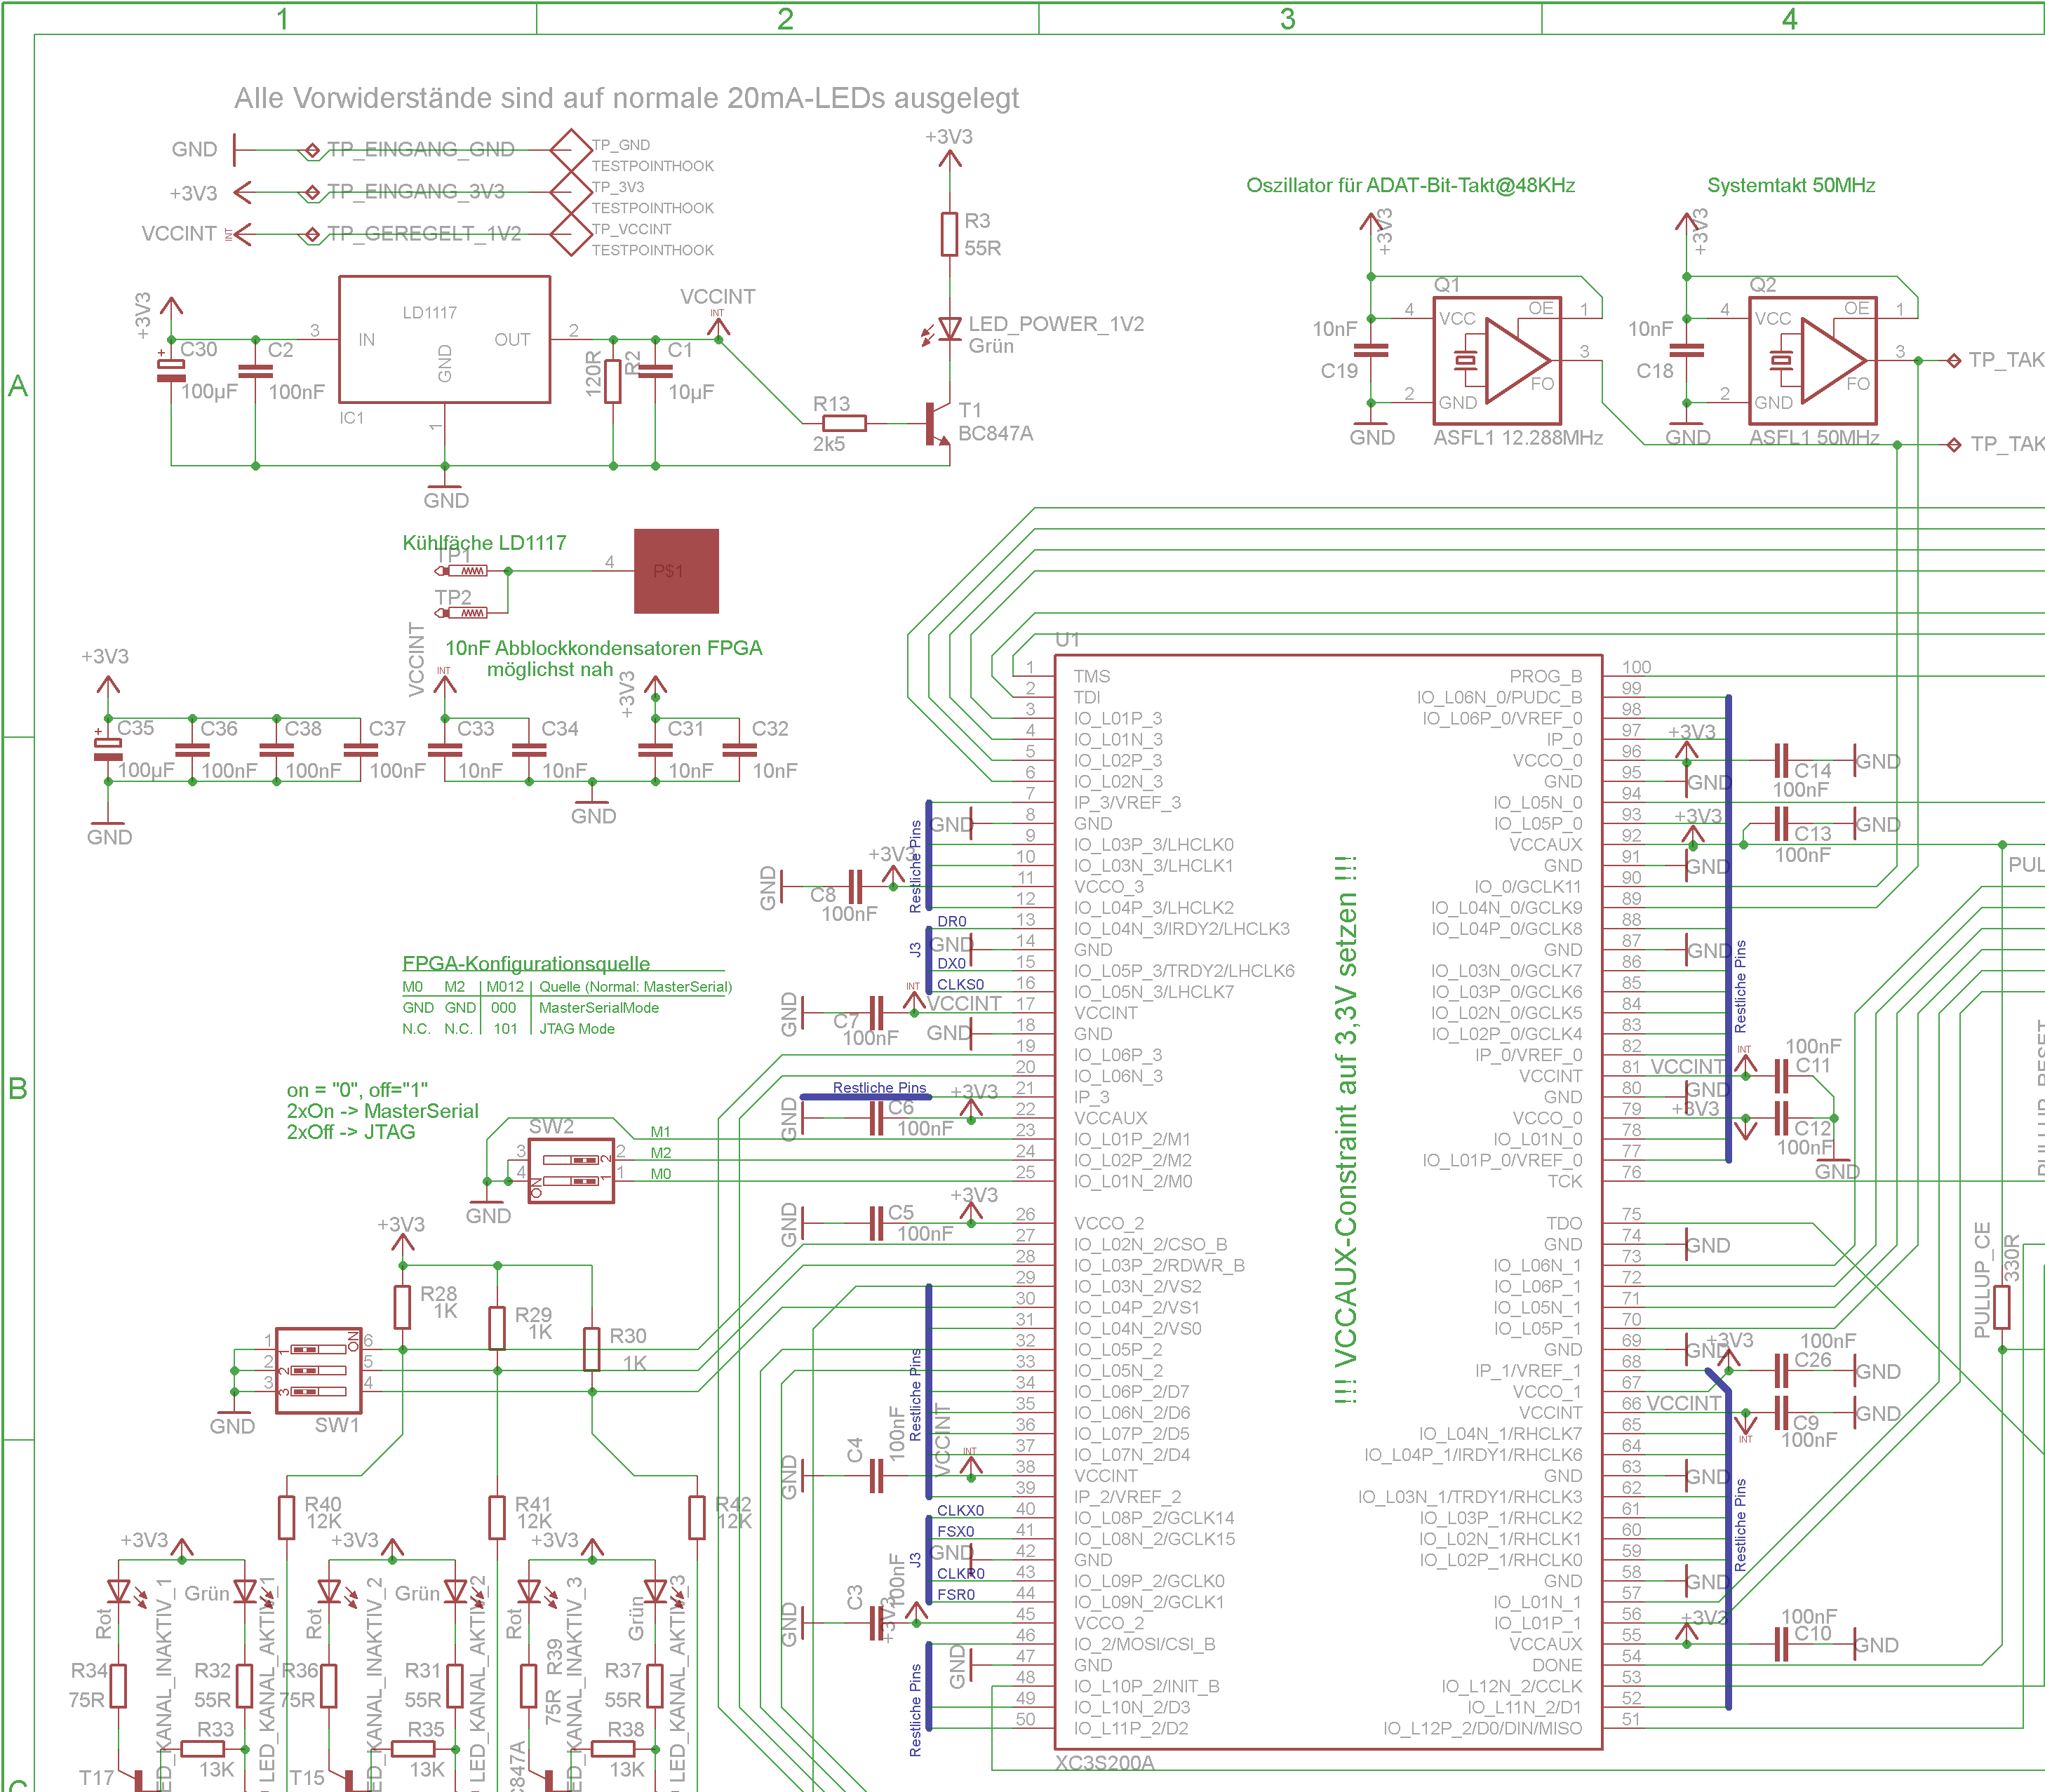
\includegraphics[width=\linewidth]{Medien/schaltplan1.png}
		\clearpage
		
		\noindent
		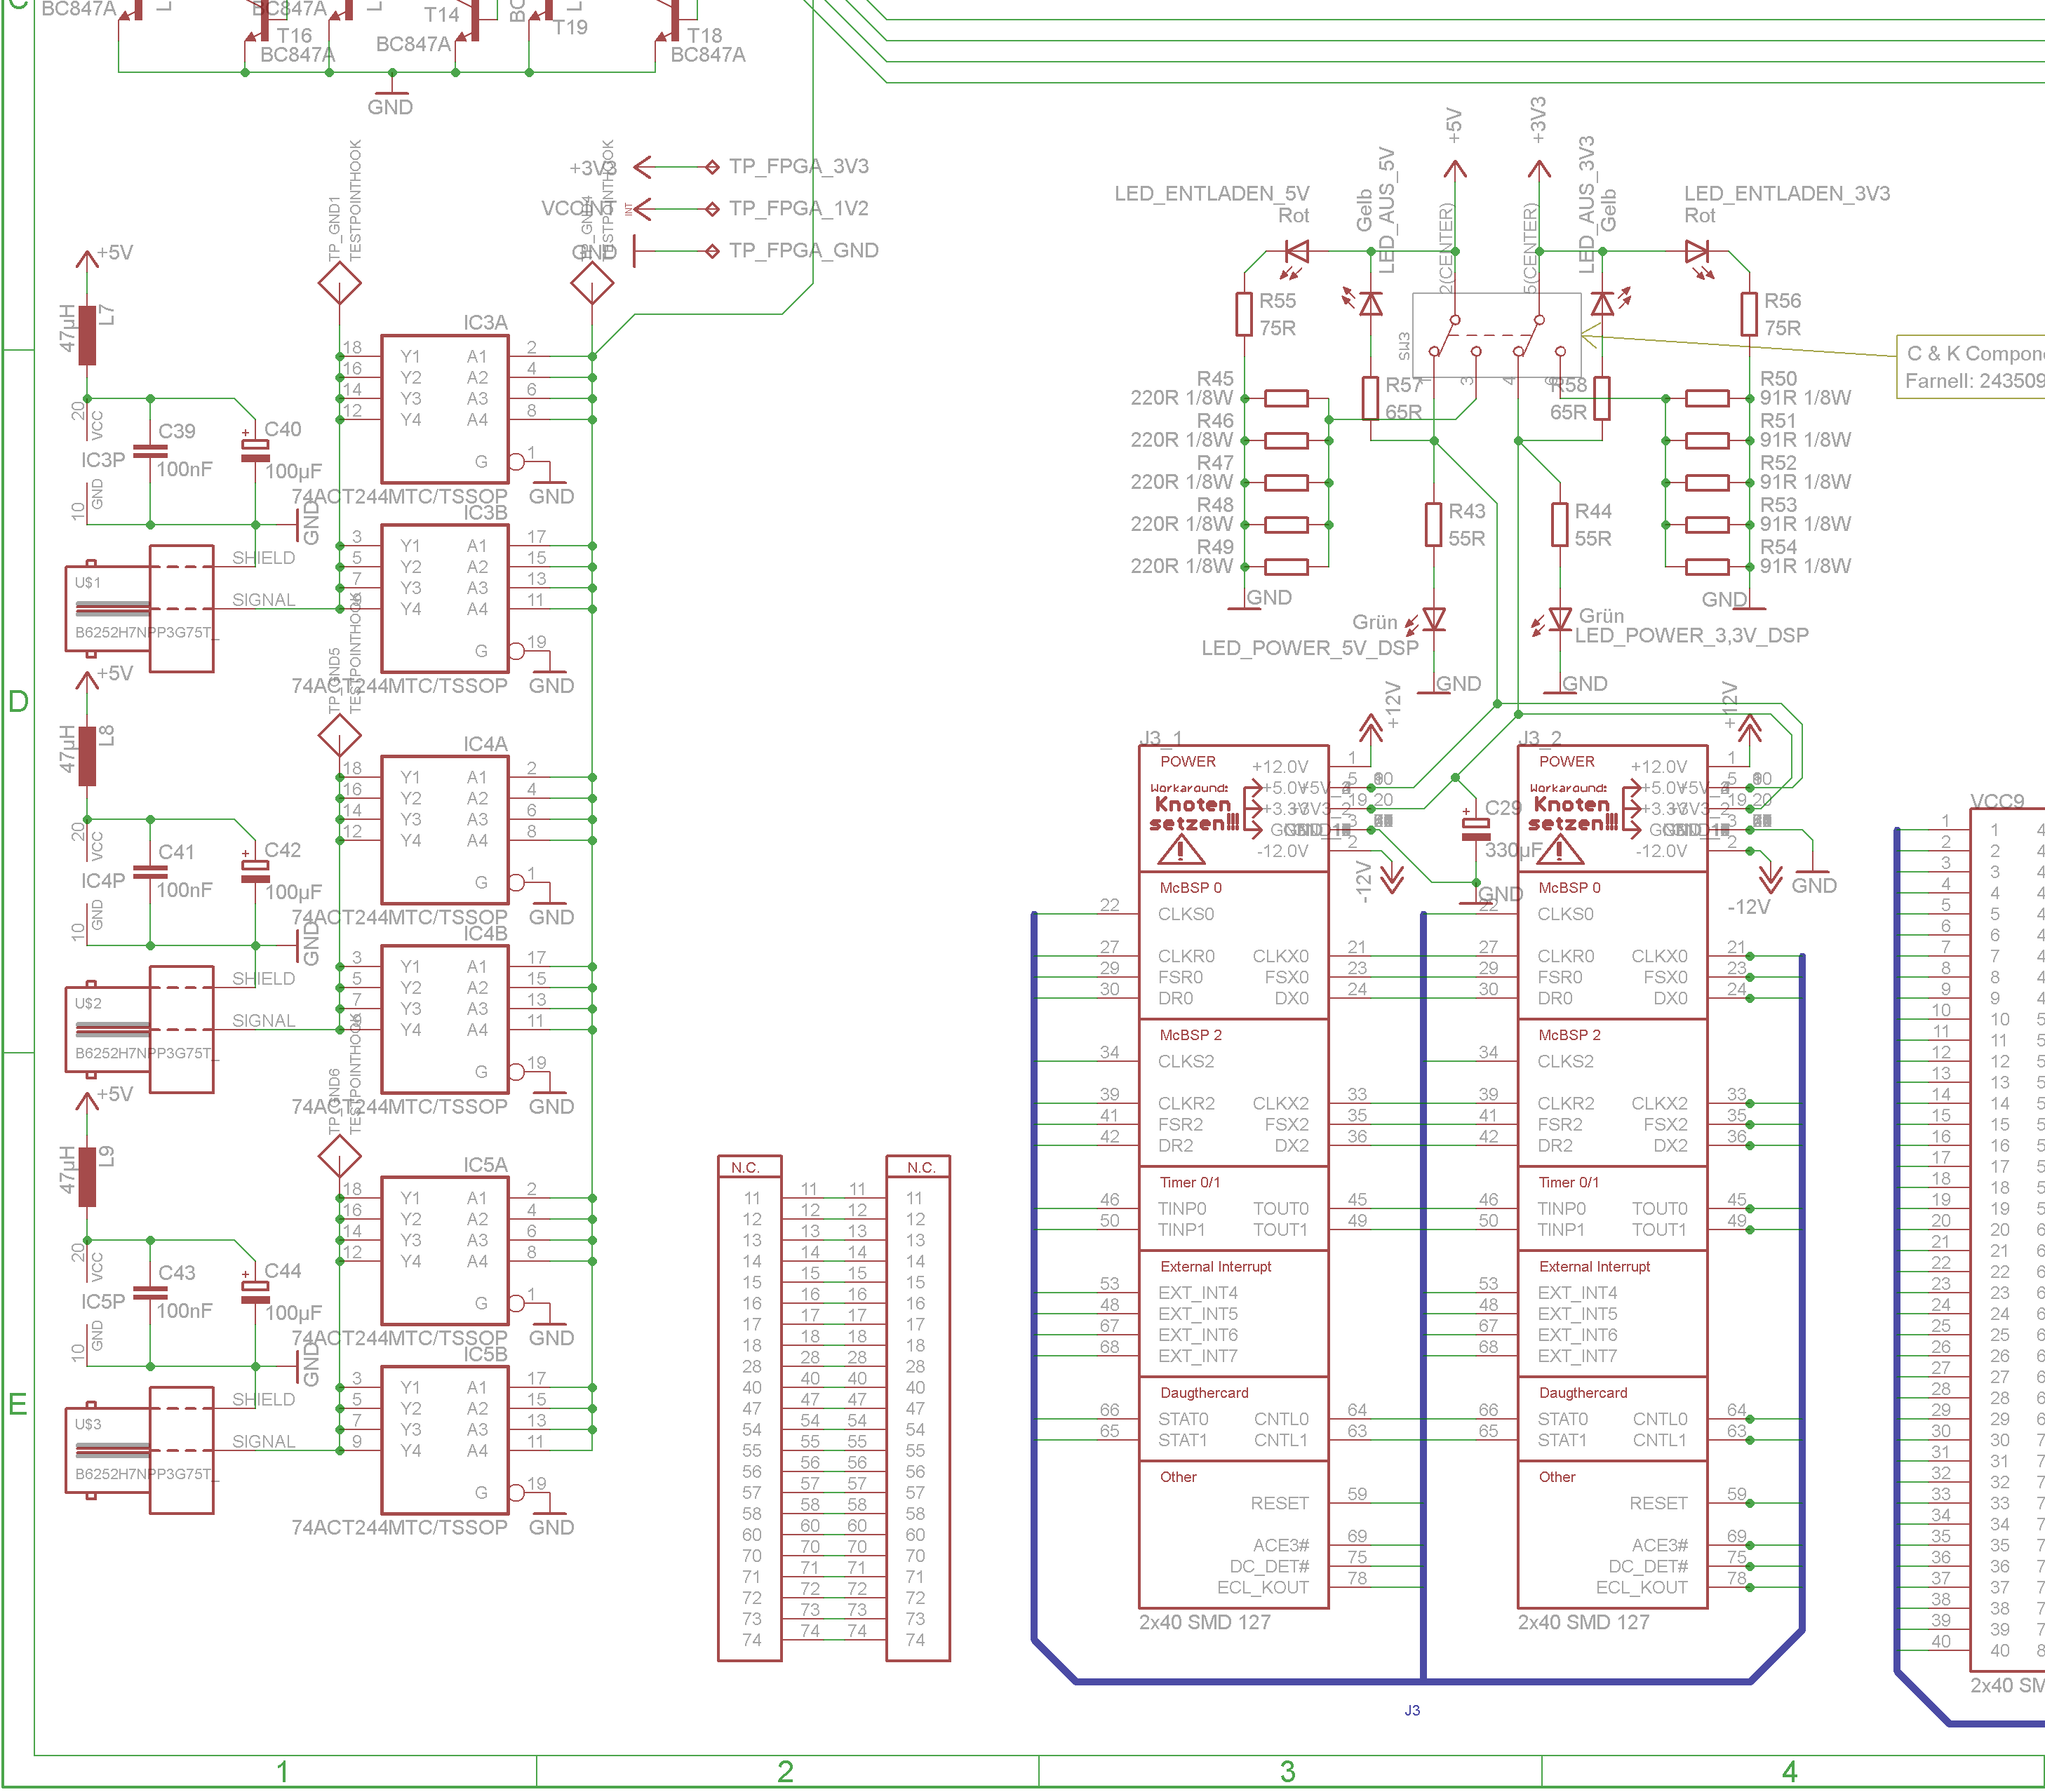
\includegraphics[width=\linewidth]{Medien/schaltplan2.png}
		\clearpage
		 
		\noindent
		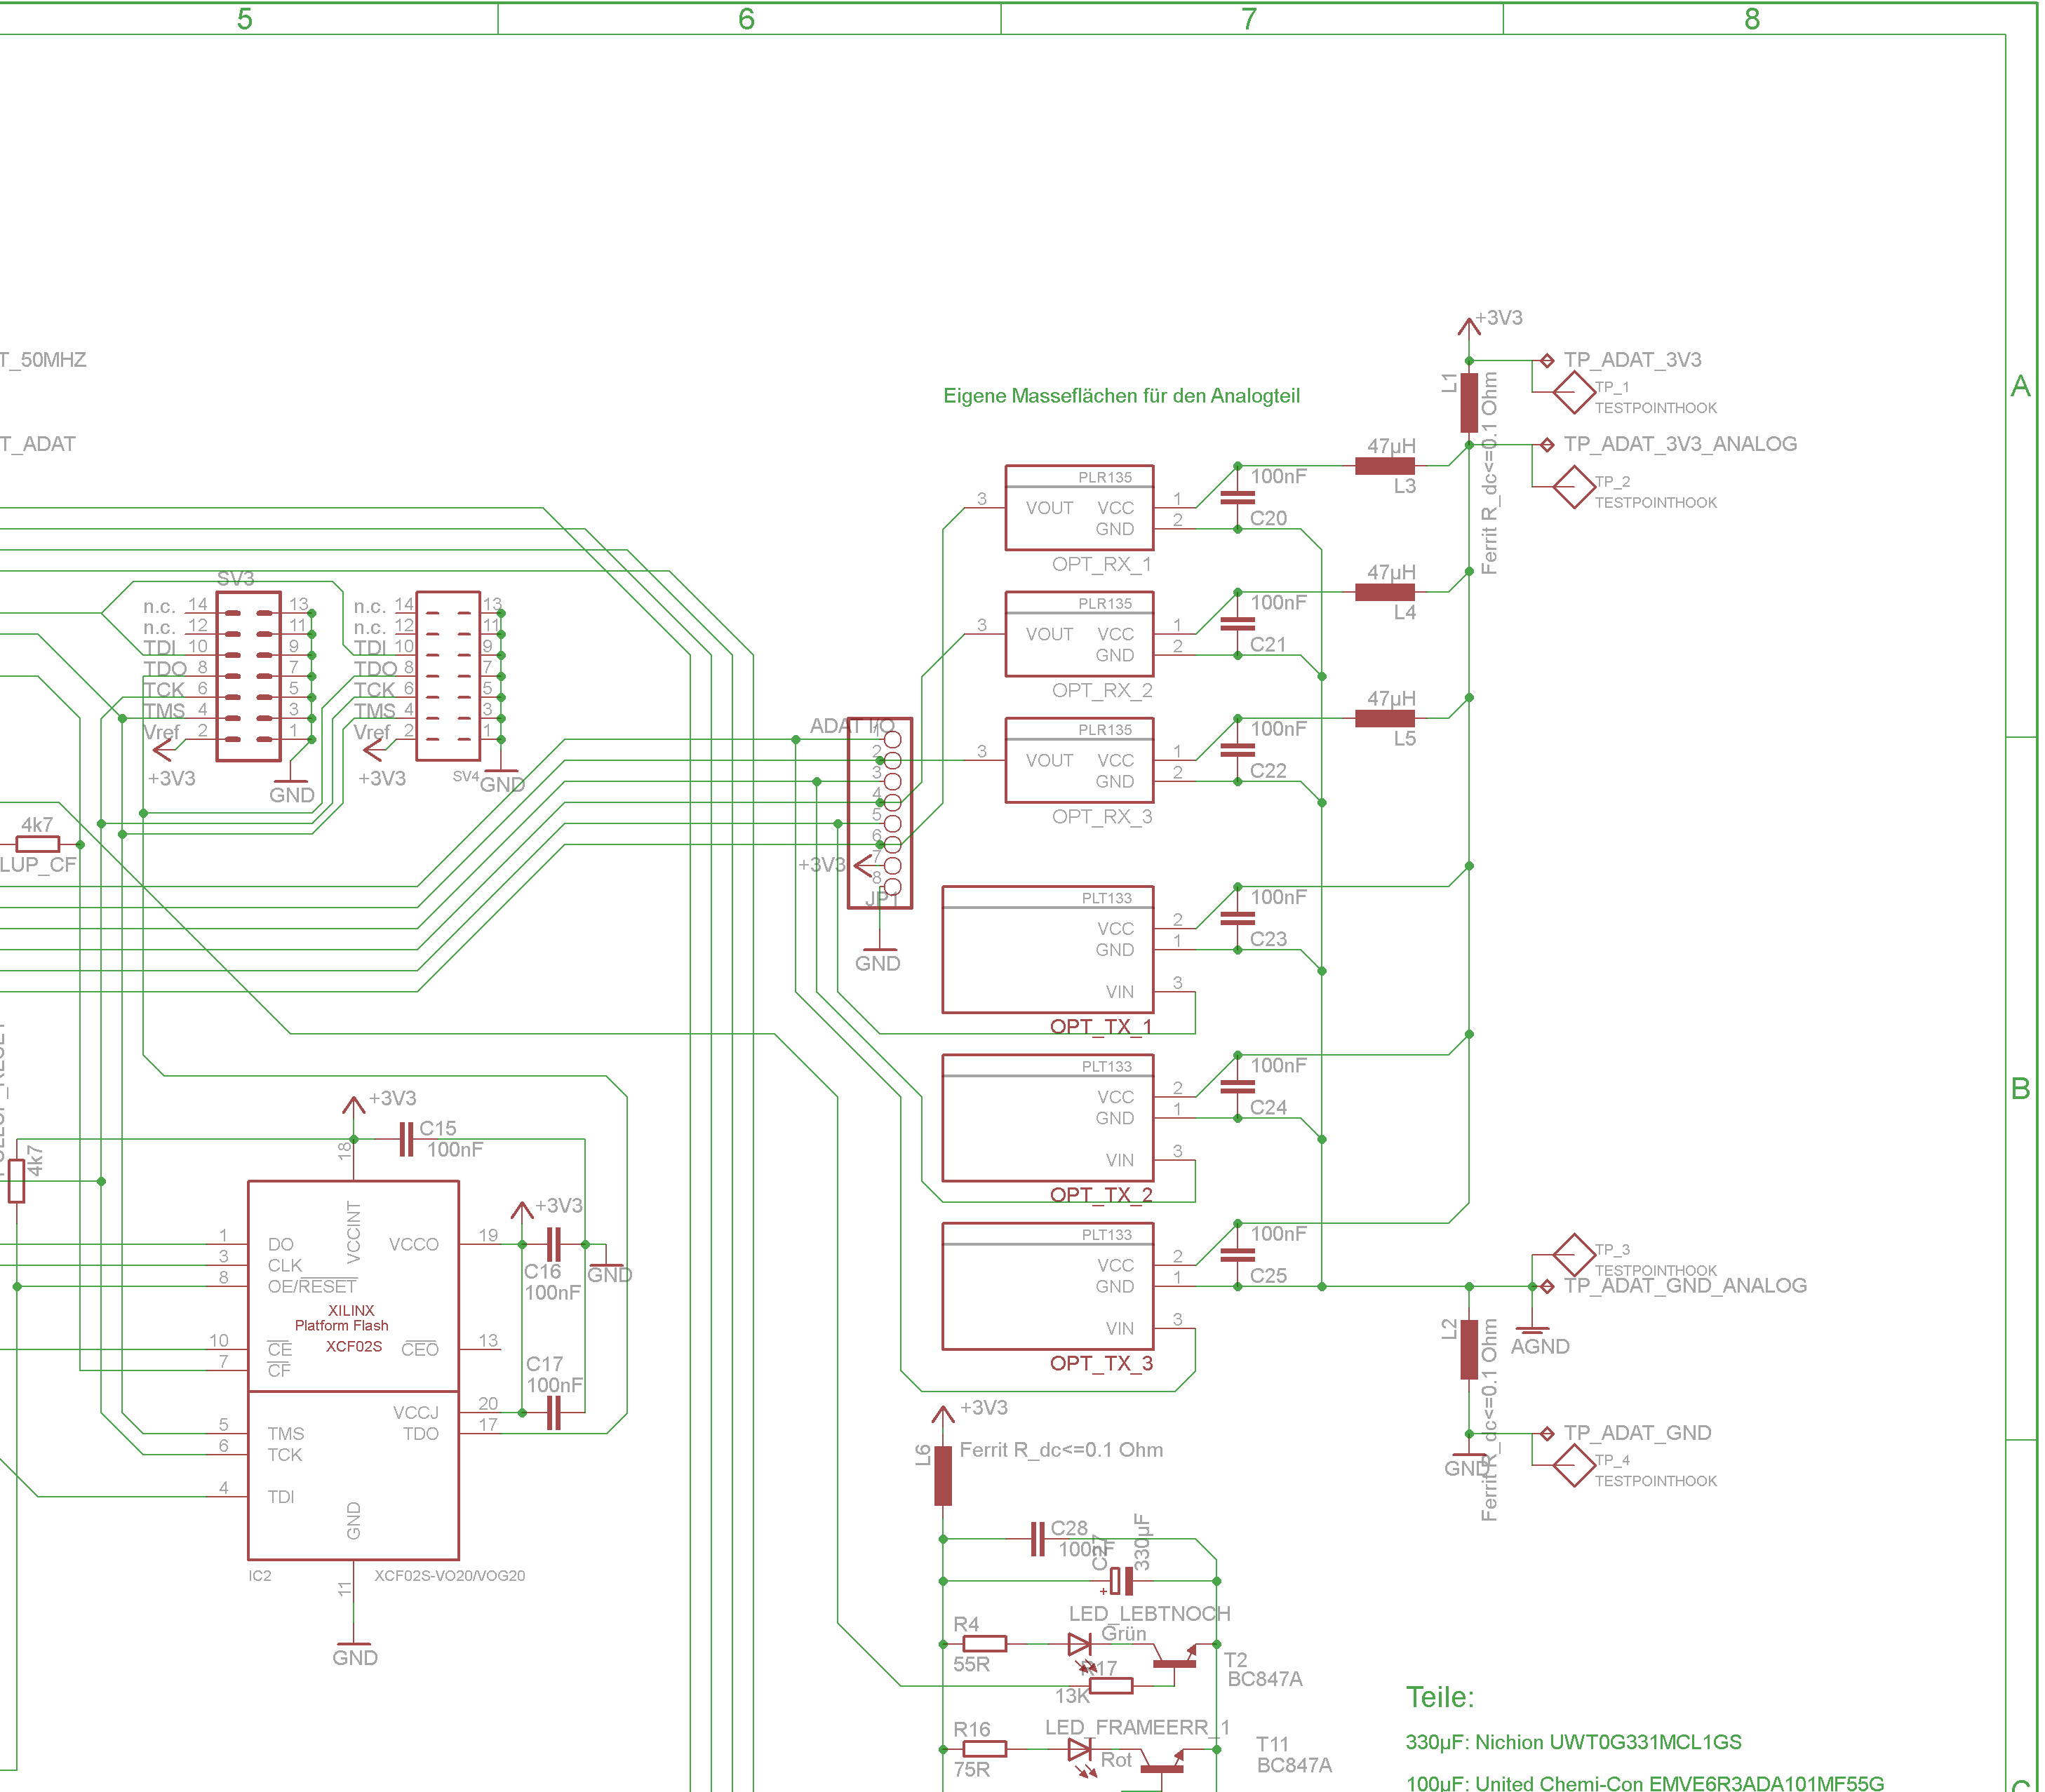
\includegraphics[width=\linewidth]{Medien/schaltplan3.png}
		\clearpage
		
		\noindent
		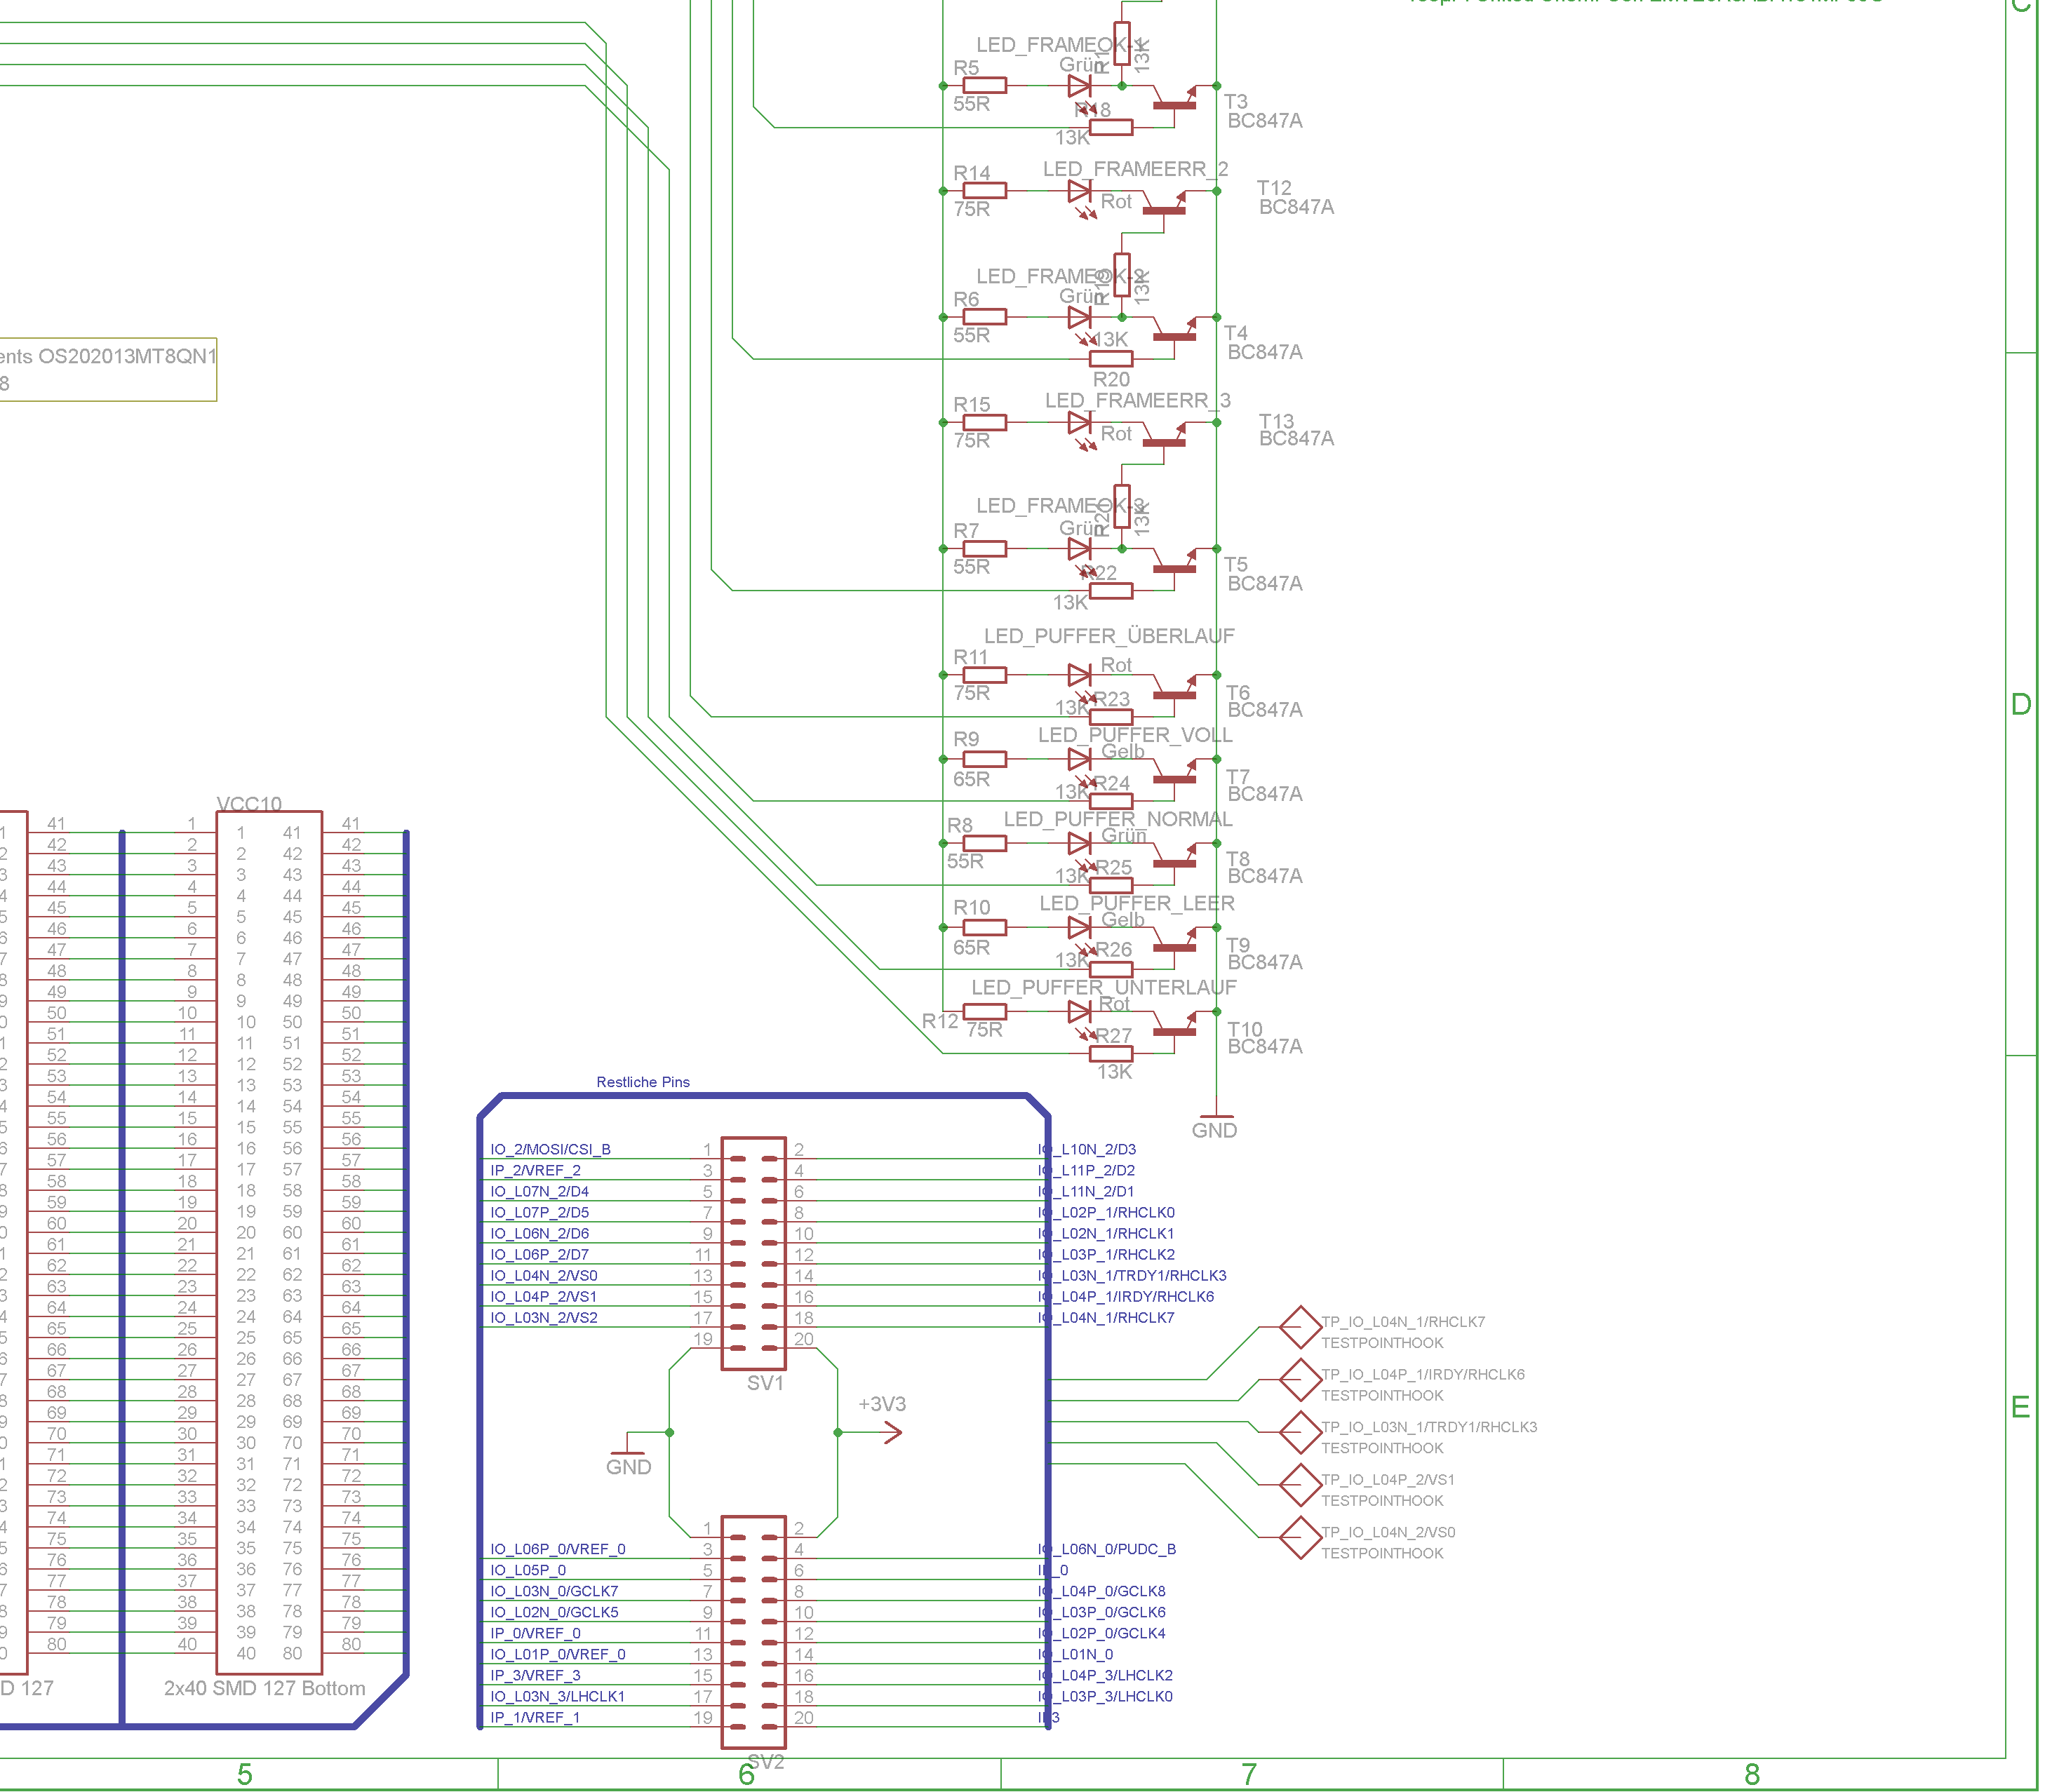
\includegraphics[width=\linewidth]{Medien/schaltplan4.png}
		\clearpage
		
		
	\section{Platinenlayout/Bestückungsplan}
		\subsection{Top Layer}
		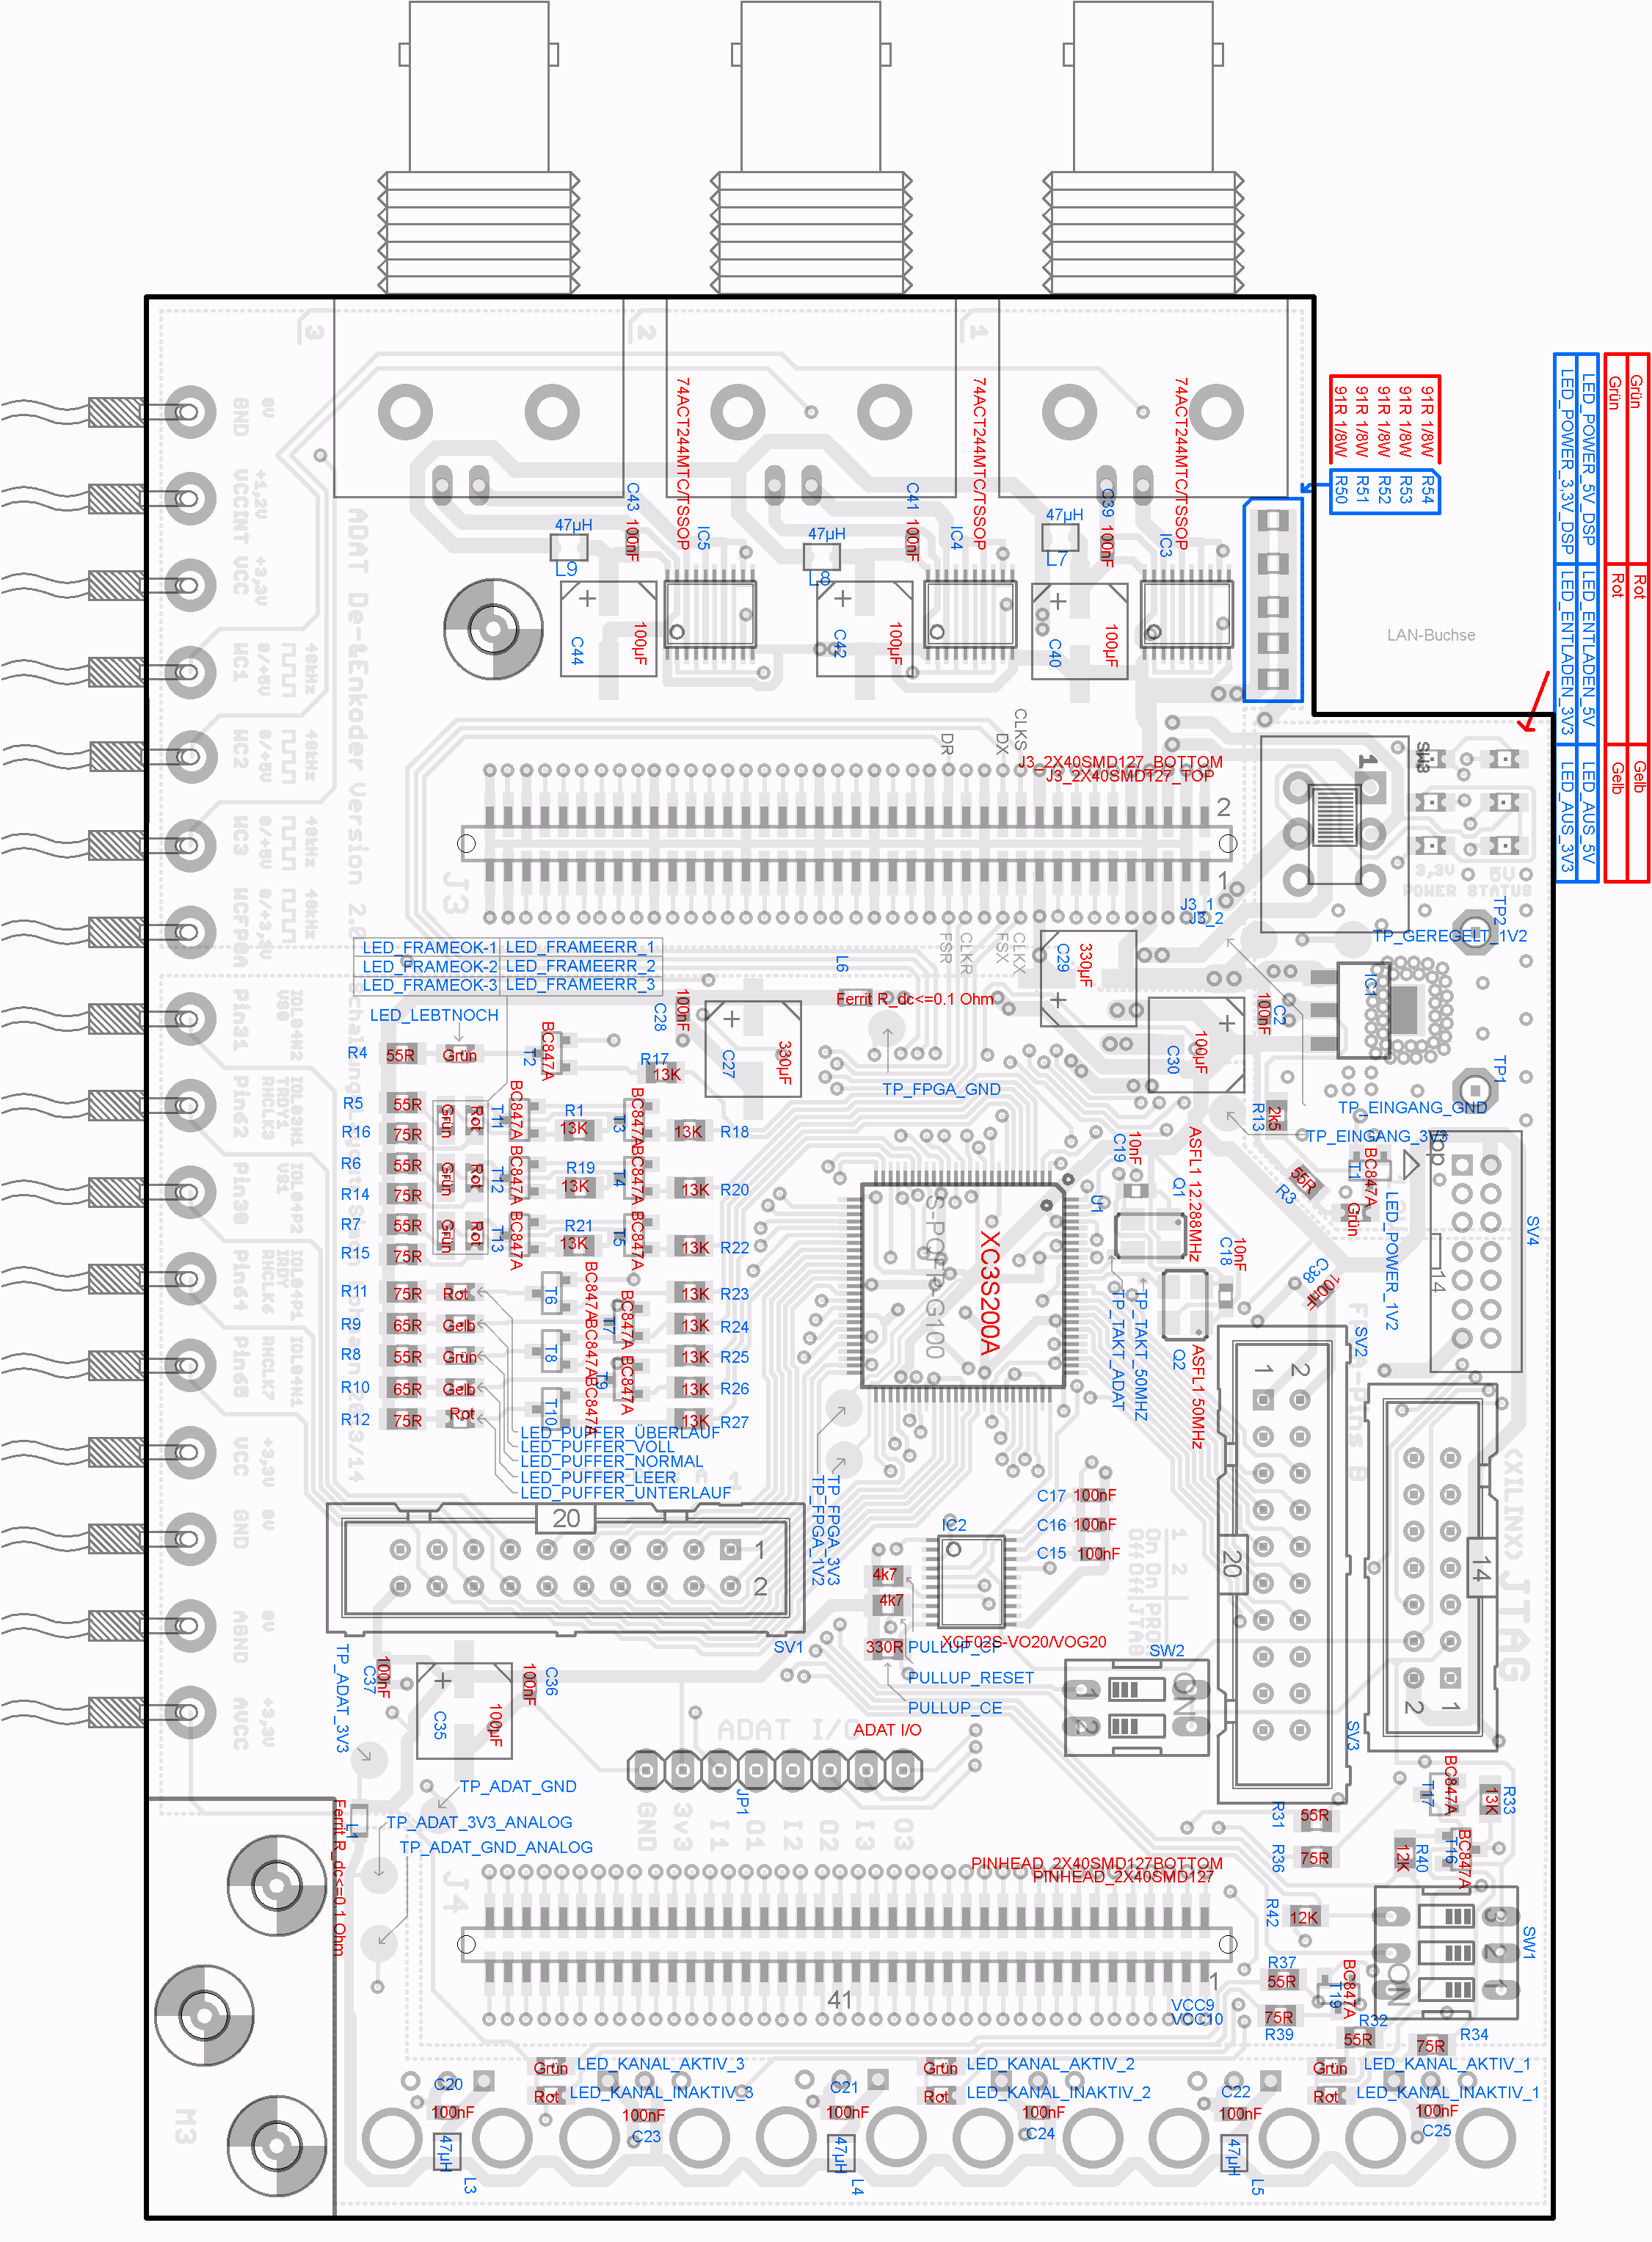
\includegraphics[width=0.85\linewidth]{Medien/bestueckungtop.png}
		\subsection{Bottom Layer}
		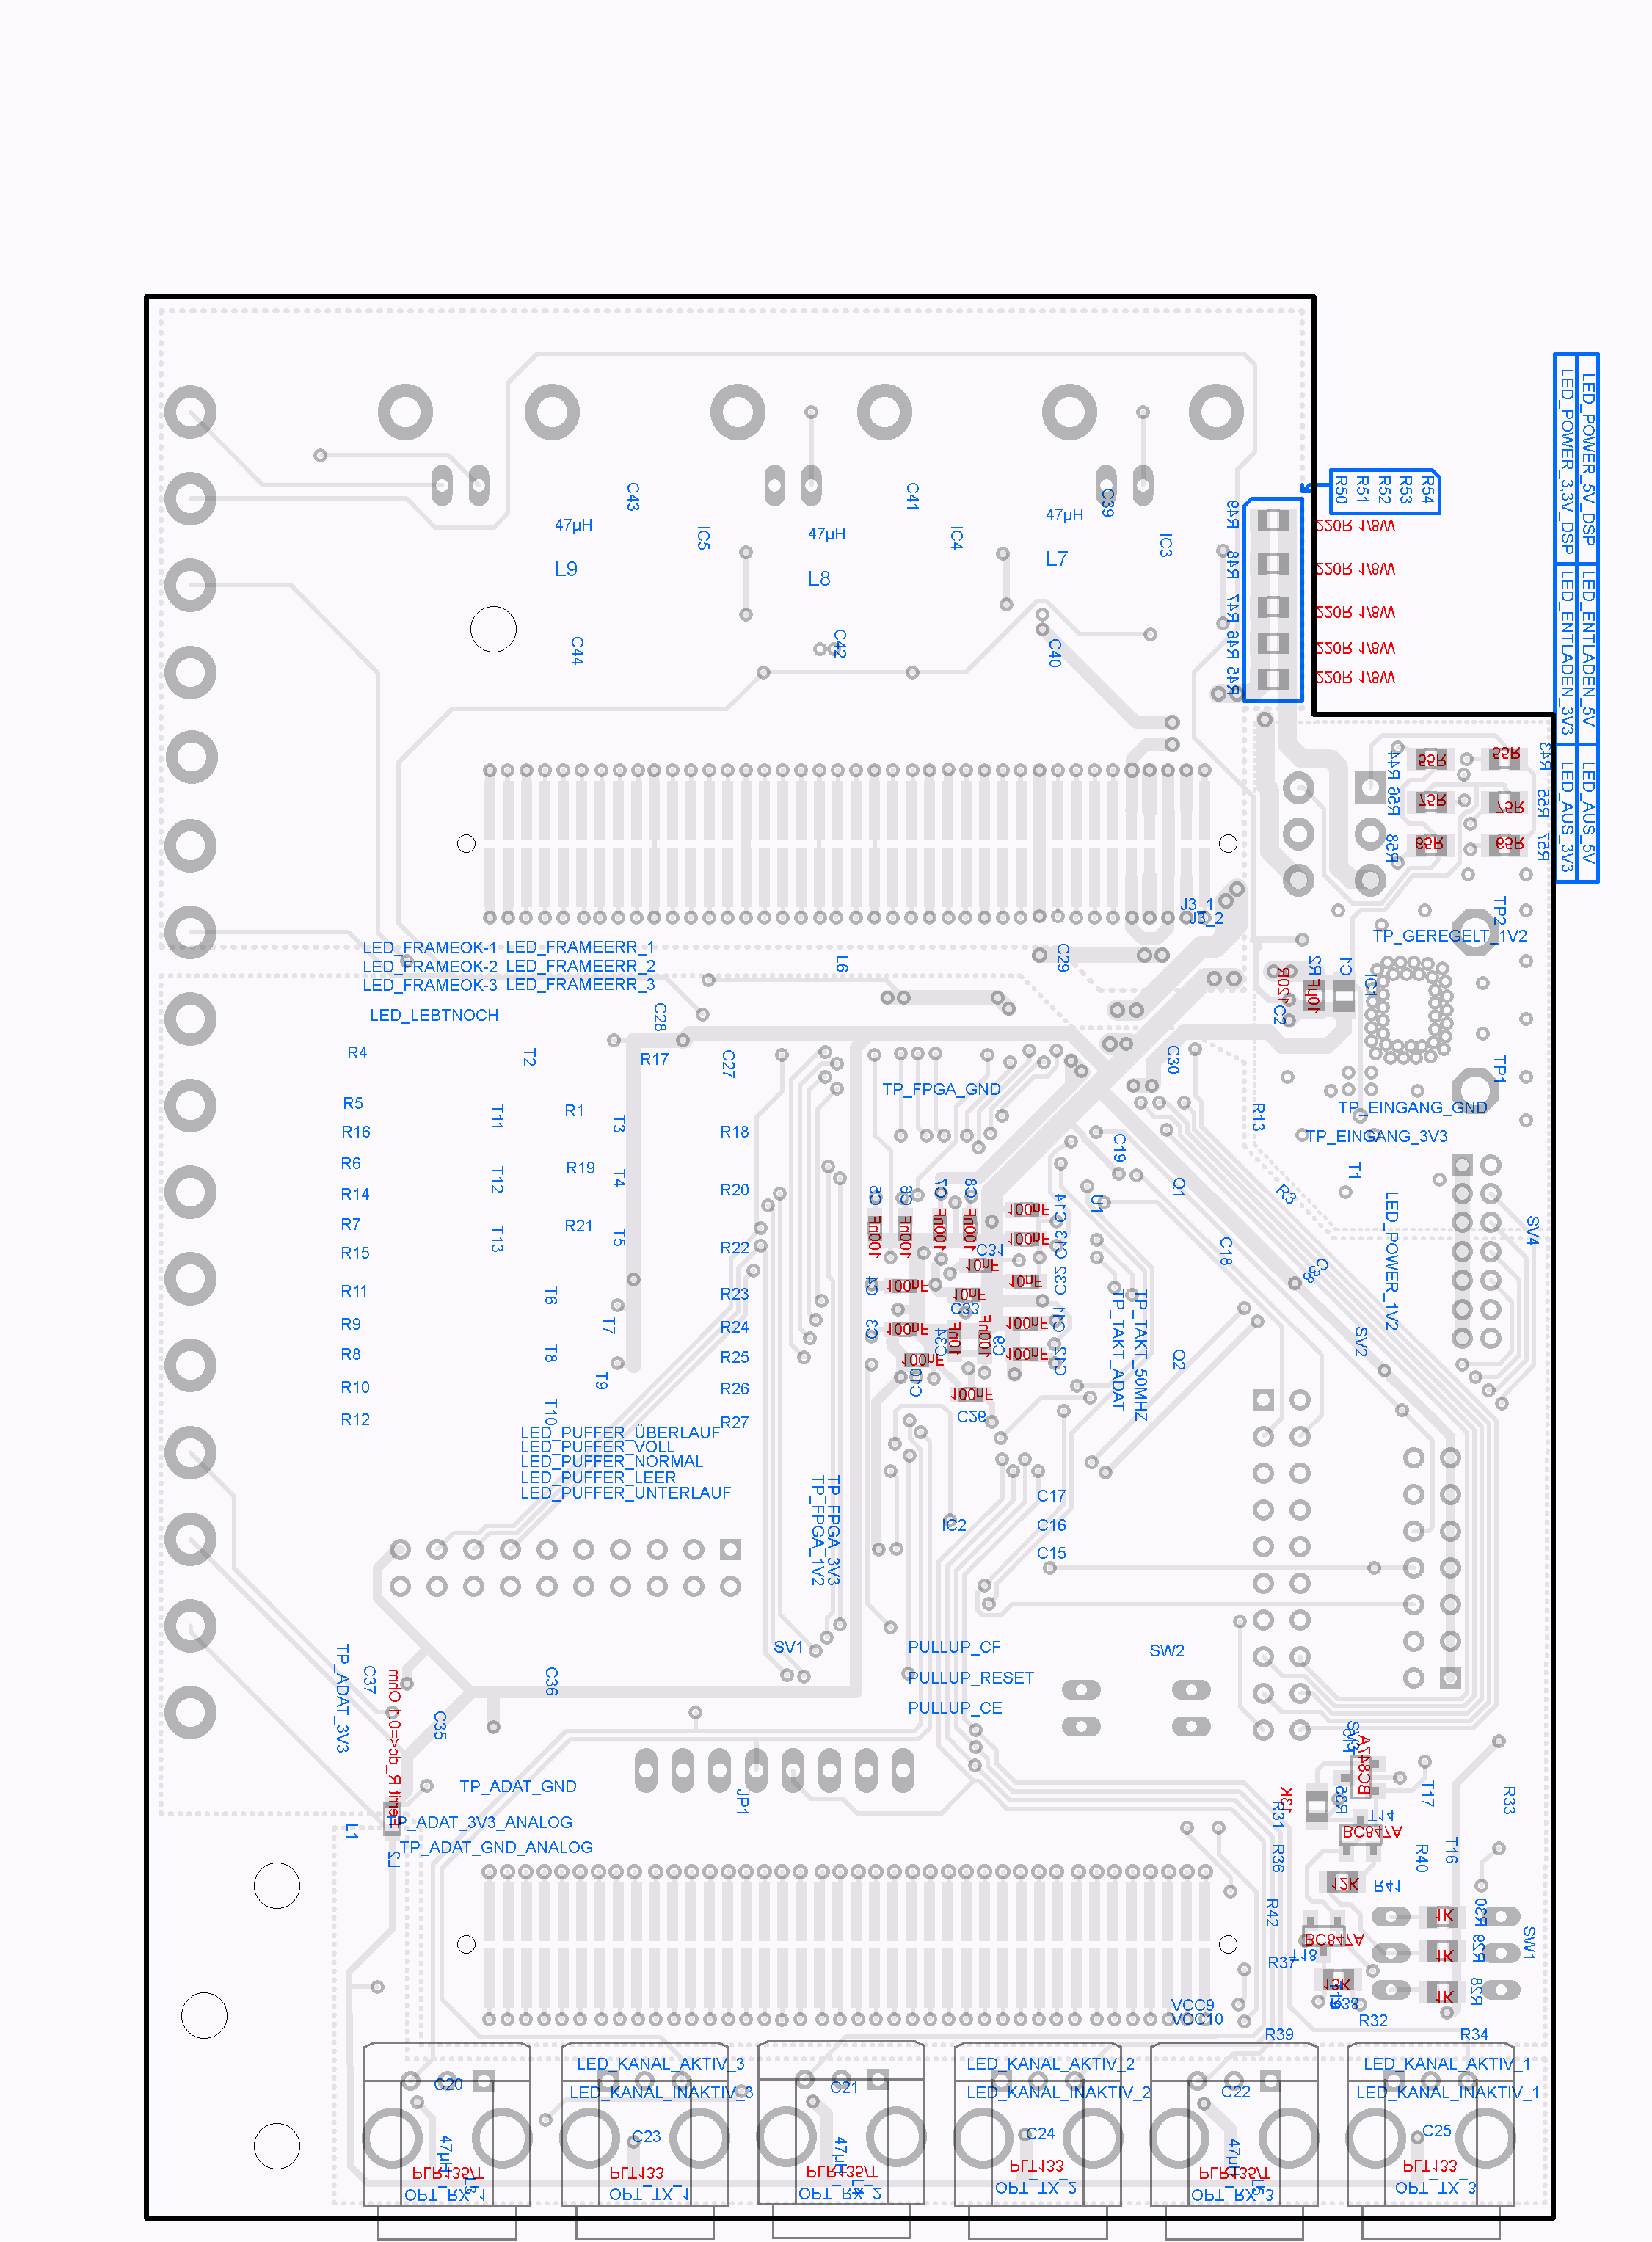
\includegraphics[width=0.85\linewidth]{Medien/bestueckungbottom.png}
	\chapter{Messreihen}
	\blindtext
	\chapter{Source Code}
	\begin{lstlisting}[language=C, caption={Ein Beispielhafter Quellcode}]
#include <stdio.h>

int main(void){
	printf("Hello World!\n");
	
	return 0;
}
	\end{lstlisting}
%   ...
	\chapter{FAQ - Frequently Asked Questions}
	\emph{engl.: Häufig stellte Fragen}
	
	\emph{In \ref{FAQ:Vorlage} gibt es die FAQ speziell zu dieser Vorlage und dem Umgang damit.}
	
	\emph{In \ref{FAQ:LaTeX} werden typische Anfängerfragen zum Thema \LaTeX{} behandelt.} 
	
	\section{Zu dieser Vorlage}\label{FAQ:Vorlage}
		\subsection{Was brauche ich?}
			\subsubsection{Diese Vorlage}
			Die Vorlage wird als komprimiertes Archiv verteilt. Dieses muss zuerst entpackt werden.
			
			\subsubsection{Eine LaTeX-Distribution}
			Je nach Betriebssystem gibt es unterschiedliche Pakete, in denen \LaTeX zusammen mit den am häufigsten benutzten Paketen zu einer sogenannten \emph{\LaTeX-Distribution} zusammengefasst ist.
%			
			\TeX Live und MiKTeX sind die am häufigsten genutzten Varianten:
			
			\paragraph{TeX Live}~\\
			\fbox{Linux} \fbox{Windows} \fbox{MacOS\footnotemark}\footnotetext{für MacOS gibt es auch noch die speziell abgestimmte Variante \emph{MacTeX}, welche auf \emph{\TeX Live} aufbaut} \fbox{FreeBSD} \fbox{NetBSD} \fbox{Solaris}
			\hfill
			\url{http://tug.org/texlive/}
			\medskip
			
			\noindent Wird in den vielen Linux-Distributionen schon mitgeliefert und über den Linux-Paketmanager automatisch aktualisiert.
			%				
			Unter Ubuntu/Mint/Debian kann man es z.B. über das Terminal mit  
			\lstinline|sudo apt install texlive| installieren.
			%				
			Je nach Anwendung gibt es verschieden große Pakete. Mit \lstinline|texlive| installiert man ein einfaches TeX-System mit häufig genutzten Paketen. Dies ist für die meisten Anwendungsfälle ausreichend.
			%				
			\lstinline|texlive-base| wäre die Minimalinstallation, alle weiteren Pakete müssen von Hand installiert werden.
			%				
			\lstinline|texlive-full| enthält alle Pakete. Dafür braucht es natürlich auch am meisten Speicherplatz.
			
			\paragraph{MiKTeX}~\\
			\fbox{Linux} \fbox{Windows} \fbox{MacOS}
			\hfill
			\url{https://miktex.org/download}
			
			\noindent Lädt Pakete nur auf Anfrage, braucht also potenziell weniger Speicherplatz.
			Bei der Installation wird gefragt, was passieren soll, wenn MiKTeX bemerkt dass ein Paket fehlt:
			\begin{description}
				\item[Nicht installieren] Fehlende Pakete werden nicht automatisch installiert -- das muss man also selber machen. \textit{(Für Anfänger nicht empfohlen)}
				\item[Nachfragen] Sobald ein Paket fehlt, öffnet MiKTeX ein Fenster in dem man auswählen kann, ob das Paket installiert werden darf. Einfach und transparent. Am Anfang wird man aber möglicherweise ziemlich oft gefragt, bis alle Pakete heruntergeladen wurden.
				\item[Automatisch installieren] Fehlende Pakete werden ohne Nachfrage beim Nutzer automatisch installiert. Einfach, aber intransparent.
			\end{description}
			
			Man kann diese Option in den Einstellungen von MiKTeX auch später noch ändern.
			
			\subsubsection{Einen (LaTeX-) Editor}
			\emph{Weil \LaTeX-Quellcode auch nur ganz normaler Text ist, kann im Prinzip jeder beliebige Text-Editor\footnote{Nur bitte nicht Word, Writer etc. Das sind keine Text-Editoren!} benutzt werden.}
			\medskip
			
			Viel einfacher (und übersichtlicher) wird es aber, wenn man einen \LaTeX-Editor benutzt.
			Diese Programme kennen in der Regel die meisten Befehle und können diese automatisch vervollständigen, bieten Vorschaufunktionen, einfaches Kompilieren und vieles mehr.
			
			
			Empfehlenswert ist z.B. \emph{TeXstudio\footnote{\url{https://www.texstudio.org/}, verfügbar für Linux, Windows \& Mac OS}}, in dem ich diesen Text hier gerade schreibe und schon diverse Vorlagen und Pakete entwickelt habe. Es enthält eine Autovervollständigung der gängigen \LaTeX-Befehle, eine einfache Rechtschreibprüfung und viele Hilfsfunktionen zum Finden von Symbolen, Formatieren von Tabellen und so weiter...
			\medskip
			
			\emph{Besonders praktisch finde ich die Option, direkt per Strg+Klick im PDF an die entsprechende Stelle im Quellcode zu springen (das geht natürlich auch anders herum). Oder mit Strg+Klick auf einen Paketnamen die entsprechende Dokumentation zu öffnen. Oder sich z.B. die Vorschau einer Formel direkt im Quellcode anzeigen zu lassen. Und es gibt noch so viel mehr...}
			
			\subsubsection{Eine Literaturverwaltung (optional)}
			Die Literaturliste kann man in einem \LaTeX-Editor schon hinreichend gut bearbeiten.
			%			
			Literaturverwaltungsprogramme können einem die Arbeit aber erleichtern.
			%			
			Frei verfügbar ist z.B. das Programm \emph{JabRef}\footnote{Läuft unter Linux, Windows und Mac OS, \url{http://www.jabref.org/}}.
			Dieses kann auch diverse Wissenschaftliche Online-Verzeichnisse durchsuchen, eignet sich (bedingt) also auch zur Literaturrecherche.
		
			
		\subsection{Titelblatt und Einstellungen ändern}\label{FAQ:Einstellungen}
			Die für Benutzer gedachten Einstellungsmöglichkeiten finden sich in der Datei \lstinline|Einstellungen.tex|.
%			
			Damit kann man \zb{} die Angaben auf der Titelseite ändern, zwischen einseitigem und doppelseitigem Layout wählen oder entscheiden, welche Verzeichnisse generiert werden sollen und vieles mehr. Alle Optionen sind dort ausführlich kommentiert.
			
		\subsection{Literatur/Quellen}
			Die Literatureinträge werden von dieser Vorlage aus der Datei \lstinline|Literatur.bib| geladen.
			Hat sich etwas an dieser Datei geändert, muss das Literaturverzeichnis neu kompiliert werden. (siehe \ref{FAQ:kompilieren:literatur} \emph{\nameref{FAQ:kompilieren:literatur}})
			
		\subsection{Glossareinträge, Abkürzungen, Akronyme}
			werden in der Datei \lstinline|Glossar.tex| eingetragen.
		
		\subsection{Im PDF sind am Anfang mehrere leere Seiten}
			Je nachdem ob Ihr in \lstinline|Einstellungen.tex| das einseitige oder das doppelseitige Layout gewählt habt, werden leere Seiten zwischen Kapiteln generiert.
			Das sieht im PDF erst mal seltsam aus, ist aber Absicht:
			%		
			So fängt \zb{} der Inhaltsteil auf der rechten Seite an (das ist eine übliche Konvention).
			Damit dann auf der linken Seite nicht noch der Rest vom Inhaltsverzeichnis steht, was schon mal etwas seltsam aussehen kann, wird dafür gesorgt, dass die erste linke Seite vor dem Start des Texts leer ist. Endet das Inhaltsverzeichnis auf der linken Seite, ergibt sich zusätzlich noch eine leere rechte Seite.
			
			Bei Aufgabenstellung, ggf. Verlängerung und Eidesstattlicher Erklärung handelt es sich jeweils um allein stehende Elemente, daher wird auch hier jeweils dafür gesorgt, dass die linke Seite daneben leer bleibt.
		
		\subsection{Seitenränder springen hin und her}
			Im doppelseitigen Layout gibt es einen inneren und einen äußeren Rand.
			\medskip
			
			\textit{In den \hyperref[FAQ:Einstellungen]{Einstellungen} kann bei Bedarf auch ein einseitiges Layout gewählt werden.}
		
		\subsection{Seitenzahlen springen hin und her}
			Im doppelseitigen Layout gibt es einen inneren und einen äußeren Rand.
			Die Seitenzahlen stehen immer am äußeren Rand der Seite.
			\medskip
			
			\textit{In den \hyperref[FAQ:Einstellungen]{Einstellungen} kann bei Bedarf auch ein einseitiges Layout gewählt werden.}
			
		\subsection{Die Druckerei zählt S/W-Seiten als Farbseiten}
			\textit{Farbseiten sind meist deutlich teurer als Schwarz-Weiß bzw. Graustufen-Seiten.
			Es kann also sinnvoll sein, wenn nur die Seiten mit farbigen Bildern etc. als Farbseiten gedruckt werden. Viele Thesis-Druckereien und Copyshops haben dafür eine Software, die Farbseiten automatisch erkennen kann\footnote{Oder das zumindest können sollte ;-)}.}
			
			Meistens funktioniert das mit dieser Thesisvorlage einwandfrei.
			Einige wenige Druckereien verhalten sich diesbezüglich aber \emph{etwas seltsam}.
			Falls eure Druckerei Probleme macht, könnt ihr in der Datei \emph{Einstellungen.tex} den Parameter \lstinline|\colormodel| anpassen.
			
			Faustregel für \lstinline|\colormodel|:
			\begin{itemize}
			\item erst mal bei der Standardeinstellung \lstinline|cmyk| lassen. Das ist das professionelle Druckformat.
			\item wenn die Druckerei Probleme macht, auf \lstinline|rgb| umstellen. Hat in einem uns bekannten Fall schon mal geholfen.
			\item wenn die Druckerei immer noch Probleme macht, auf \lstinline|gray| umstellen.
			\end{itemize}

	\clearpage
	\section{Zu \LaTeX{} allgemein}\label{FAQ:LaTeX}
		\subsection{Hintergrundwissen: Aus \LaTeX{} wird ein PDF}
			\LaTeX-Quellcode wird kompiliert, dass heißt ein spezielles Programm (der \emph{Compiler}) liest den Quellcode und erstellt daraus ein Dokument im Zielformat.
			Je nach Compiler und dessen Einstellungen können dabei unterschiedliche Zielformate herauskommen.
%			
			Einer der wichtigsten Compiler ist \emph{Pdf\LaTeX}. Er erstellt aus dem Code ein PDF-Dokument. Dieses kann dann einfach betrachtet, gedruckt, kommentiert oder auf einem Datenträger der Thesis beigelegt werden.
			
			\emph{Praktisch alle Druckereien nehmen PDF-Dokumente an.
			Mit einem Writer- oder Word-Dokument, LaTeX-Code oder anderen Datei-Formaten wollen die Druckereien dagegen häufig lieber nichts zu tun haben\footnote{Im schlimmsten Fall wird der Druckauftrag abgelehnt, wenn es etwas besser läuft müsst Ihr evtl. einen Aufpreis zahlen. Mit einem PDF seid Ihr dagegen bei praktisch allen seriösen Anbietern auf der sicheren Seite.}}
			
		\subsection{\LaTeX{} kompilieren}
			Die Thesis kann im Terminal mit dem Befehl \lstinline|pdflatex Thesis.tex| kompiliert werden.
			In \emph{TeXstudio} geht das mit einem Klick auf den Kompilieren-Button oder mit der Taste \fbox{F5}.
			
			In manchen Fällen muss man zwei mal kompilieren, mehr dazu in Abschnitt \ref{FAQ:kompilieren:zweimal} \emph{\nameref{FAQ:kompilieren:zweimal}}.
		\subsection{Literaturverzeichnis kompilieren}\label{FAQ:kompilieren:literatur}	
			Das Literaturverzeichnis wird in der Regel von einem separaten Programm verarbeitet (z.B. BibTeX, BibLaTeX oder Biber).
			%In dieser Thesisvorlage wird BibLaTeX verwendet, das Backend ist BibTeX (so passen die Standardeinstellungen von TeXstudio direkt).
			\medskip
			
			Dieses muss explizit aufgerufen werden.
			In \emph{TeXstudio} geht dass z.B. mit der Taste \fbox{F8}, im Terminal per \lstinline|bibtex Thesis.aux|.
			
			Danach muss dann das \LaTeX-Dokument (in \emph{TeXstudio} mit \fbox{F5}) kompiliert werden.
			\bigskip
			
			\hrule
			\medskip
			\noindent \textbf{Im Worstcase\footnote{alles hat sich geändert} muss man}:
			\begin{enumerate}
			\item \LaTeX-Code kompilieren \emph{(damit bekannt ist, welche Quellenverweise es gibt)}
			\item Literatur kompilieren \emph{(Quellen zusammenstellen)}
			\item \LaTeX-Code kompilieren \emph{(Layout des Dokuments, Verzeichnisse vorbereiten)}
			\item \LaTeX-Code kompilieren \emph{(Verzeichnisse korrekt setzen)}
			\end{enumerate}
			In der Praxis ist das aber kein großes Problem, da man beim Arbeiten an dem Dokument meist nach Bedarf kompiliert...
			\hrule
		
		\subsection{Zwei mal kompilieren}\label{FAQ:kompilieren:zweimal}
			\textit{
				\begin{itemize}\itemsep=0pt
					\item Das neue Kapitel ist nicht im Inhaltsverzeichnis aufgeführt?
					\item Der Verweis auf ein Bild zeigt auf die falsche Seite?
				\end{itemize}
			}
			
			\begin{center}
				Lösung: Einfach zwei mal kompilieren.
				\bigskip
				
				Aber warum eigentlich?
			\end{center}
			
			
			Normalerweise wird der \LaTeX-Code einmal von vorne nach hinten durchgegangen und dabei kompiliert.
%			
			Am Beispiel des Inhaltsverzeichnis wird direkt klar, dass damit bestimmte Dinge nicht möglich sind:
				Wenn das Inhaltsverzeichnis vorne im Dokument gesetzt werden soll, weiß \LaTeX{} zu diesem Zeitpunkt noch gar nicht, auf welcher Seite die Kapitel stehen werden und welche Kapitel es überhaupt gibt -- schließlich folgen diese erst später im Quellcode.
			
			Stattdessen läuft der \LaTeX-Compiler einmal durch das gesamte Dokument und merkt sich dabei, welche Kapitel existieren und auf welchen Seiten diese begonnen haben.
				Diese Information wird dann in eine Datei gespeichert\footnote{Deshalb liegen neben dem eigentlichen \LaTeX-Dokument und der Literaturdatei nach dem kompilieren noch so viele andere Dateien mit Endungen wie z.B. \lstinline|.aux| oder \lstinline|.toc| herum}.
%			
			Im zweiten Durchlauf werden diese Informationen wieder eingelesen und verwendet um das Inhaltsverzeichnis zu erstellen, d.h. das Inhaltsverzeichnis hinkt quasi einen Kompilierschritt hinterher.
			\bigskip
			
			\noindent Das gleiche gilt auch für
			\begin{itemize}
			\item Verweise/Referenzen (bzw. alles was mit Seitenzahlen zu tun hat)
			\item alle anderen Verzeichnisse, z.B. Abbildungsverzeichnis, Tabellenverzeichnis, Literaturverzeichnis.
			\end{itemize}
		
		

		
		\subsection{Floating-Umgebungen}\label{sec:wissen:float}
			\textit{Hilfe, mein Bild/meine Tabelle/... ist nicht wo es sein soll!} --
	%		
			Bilder, Tabellen usw. sind in \LaTeX{} sogenannte \emph{Floating-Umgebungen}, d.h. sie sind nicht fest an einem Platz, sonderen werden beim Kompilieren so verschoben, dass die Seite gut aussieht.
	%		
			Nun ist \emph{was gut aussieht} nicht unbedingt für jeden gleich, und es gibt auch Fälle in denen \LaTeX{} sich scheinbar sehr seltsam entscheidet.
			Daher kann man in eckigen Klammern ggf. Präferenzen für die Positionierung angeben, die \LaTeX{} dann als Orientierung nimmt - im Zweifelsfall aber auch ignorieren darf:
			
			\begin{description}
			\item[t] bitte oben auf die Seite
			\item[b] bitte unten auf die Seite
			\item[h] bitte hier an dieser Stelle im Text
			\item[p] bitte auf eine eigene Seite packen, auf der nur andere Floats sein dürfen
			\item[!] \LaTeX soll seine eigenen Regeln zum guten Platzieren von Floats ignorieren
			\end{description}
		
	
		

		
		\subsection{Leerzeichen nach einem Befehl fehlt}
			\subsubsection*{Das Problem}
				Schreibt man einen Satz wie z.B. \emph{Ich benutze \LaTeX, weil \LaTeX für Formelsatz super ist.} so fällt auf, dass zwischen \emph{\LaTeX{}} und \emph{für} das Leerzeichen fehlt.			
				Habe ich es einfach nur vergessen?
				
				Nein, hier ist der Quellcode:
				\bigskip
				
				\lstinline[language=thesis-latexbeispiel, showspaces=true]|Ich benutze \LaTeX, weil \LaTeX für Formelsatz super ist.|
				\bigskip
			
				Wie man sieht, steht hinter dem zweiten \lstinline[language=thesis-latexbeispiel]|\LaTeX| eindeutig ein Leerzeichen. Dieses fällt aber weg, weil Befehle in \LaTeX normalerweise grundsätzlich Parameter erwarten, also das nächste Zeichen betrachten und schauen ob noch ein Parameter kommt. Bei fettgedrucktem Text wie \lstinline[language=thesis-latexbeispiel]|dieser \textbf{Text} ist fettgedruckt| (dieser \textbf{Text} ist fettgedruckt) ist das offensichtlich, bei \lstinline[language=thesis-latexbeispiel]|\LaTeX| halt nicht. Wie man bei genauem Hinschauen sieht, ist es beim ersten \lstinline[language=thesis-latexbeispiel]|\LaTeX| auch kein Problem, weil direkt ein Komma folgt. Lediglich Leerzeichen werden von solchen Befehlen \glqq gefressen\grqq, weil ein Leerzeichen durchaus erlaubt wäre.
				
				Dieses Verhalten ist auch durchaus sinnvoll, weil man manchmal nach einem \LaTeX-Befehl vielleicht auch gar kein Leerzeichen haben will. So ist z.B. \lstinline|\LaTeXbefehl| kein gültiger \LaTeX befehl, und eigentlich wollten wir hier ja auch nur \lstinline[language=thesis-latexbeispiel]|\LaTeX| und \lstinline|befehl| aneinanderhängen. Folglich kommt zwischen \lstinline[language=thesis-latexbeispiel]|\LaTeX| und \lstinline|befehl| ein Leerzeichen, an dem \LaTeX erkennt, wo der Befehl zu Ende ist und der Text weitergeht. Weil das Leerzeichen aber nur markiert, wo der \LaTeX Befehl endet, taucht es im Text nicht auf.
			\subsubsection*{Die Lösung}
				In solchen Fällen (oder immer, es schadet jedenfalls nie) einfach \lstinline[language=thesis-latexbeispiel]|\LaTeX{}| schreiben, also leere Parameterklammern hinzufügen. So ist direkt klar, wo der Befehl aufhört und das Leerzeichen wird nicht mehr \glqq gefressen\grqq:
				\bigskip
				
				\emph{Ich benutze \LaTeX, weil \LaTeX{} für Formelsatz super ist.}
				\medskip
				
				\lstinline[language=thesis-latexbeispiel, showspaces=true]|Ich benutze \LaTeX, weil \LaTeX{} für Formelsatz super ist.|              % Fragen und Antworten zur Vorlage und zu LaTeX
	\chapter{\LaTeX-Beispiele}
	\emph{Dieses Kapitel beinhaltet Beispiele und kurze Erklärungen zu verschiedenen \LaTeX-Funktionen die in einer wissenschaftlichen Ausarbeitung nützlich sein könnten.%
%	Wie diese konkret benutzt werden, kann man im \LaTeX-Quellcode der Thesisvorlage %(Datei \lstinline|LaTeX-Beispiele.tex|)
%	 sehen.
	 }
		
	\section{Kapitel, Abschnitte, Paragraphen}\label{sec:chapter-section-paragraph}
		Kapitel werden mit \lstinline|\chapter{Kapitelname}| erstellt.
		Als nächste Ebenen folgen \lstinline|\section{title}|, \lstinline|\subsection{title}| und \lstinline|\subsubsection{title}|.
		Reicht das immer noch nicht, gibt es auch noch \lstinline|\paragraph{title}| und für den aller äußersten Notfall\footnote{Wer so viele Hierarchieebenen benötigt mach in der Regel etwas falsch -- Selbst außergewöhnlich lange Bachelor- und Master-Thesen sind normalerweise nicht so umfangreich, dass Subparagraphen nötig werden} sogar noch \lstinline|\subparagraph{title}|.
		\begin{vorlagenbeispiel}
			\subsection{Subsection}
				Hier sind wir in einer Subsection.
				\subsubsection{Subsubsection}
					Hier sind wir in einer Subsubsection.
					\paragraph{Paragraph}
						Hier sind wir in einem Paragraph.
%						\subparagraph{Subparagraph}
%							Hier sind wir in einem Subparagraph.
		\end{vorlagenbeispiel}
		
	\section{Textauszeichnung}
		\begin{vorlagenbeispiel}
			Text kann man zum Beispiel \textbf{Fett}, \textit{Kursiv} oder \underline{Unterstrichen} hervorheben. Das geht aber auch mit \textsc{Kapitälchen}, \texttt{Dicktengleicher Schrift} oder \textsf{Serifenloser Schrift}.
		\end{vorlagenbeispiel}
		\begin{lstlisting}[keywords={textbf, textit, underline, textsc, texttt, textsf}]
Text kann man zum Beispiel \textbf{Fett}, \textit{Kursiv} oder \underline{Unterstrichen} hervorheben. Das geht aber auch mit \textsc{Kapitälchen}, \texttt{Dicktengleicher Schrift} oder \textsf{Serifenloser Schrift}.
		\end{lstlisting}
					
	\section{Fußnoten}
		\begin{vorlagenbeispiel}
		Ein Text kann Fußnoten\footnote{Wie z.B. diese hier} enthalten.
		\end{vorlagenbeispiel}
		Diese werden mit \lstinline|\footnote{text}| gesetzt. Formatierungen in der Fußnote sind grundsätzlich kein Problem%
		\footnote{%
			\color{red}Dies ist eine besonders \textbf{fette Fußnote} in rot.
		}.
%		
		Aber Vorsicht: Manche Befehle wie \zb \lstinline|\lstinline| können nicht ohne weiteres/nicht immer in einer Fußnote gesetzt werden\footnote{Der Grund dafür lässt sich unter \url{https://www.texfaq.org/FAQ-verbwithin} nachlesen}.
	
	\section{Zitate \& Literaturangaben}
		\subsection{Zitieren}
			Korrektes Zitieren ist in der Wissenschaft \emph{(und auch sonst)} äußerst wichtig und daher Pflicht.
%			\medskip
%			
			Bei allem%
				\footnote{Basiswissen aus dem jeweiligen Fachbereich muss in der Regel nicht zitiert werden, d.h. ein Student der Elektotechnik muss $U = R \cdot I$ nicht zitieren, ein Kunststudent, der ein paar LEDs anschließen möchte und dafür einen Vorwiderstand berechnet, ansonsten aber noch nie etwas von dieser Formel gehört hat, sollte dies hingegen schon.}%
			, was man von anderen übernommen hat, muss angegeben werden, woher es stammt und wer es verfasst/veröffentlicht hat.
				\medskip
					
			Auf diese Weise wird eindeutig gezeigt, dass eine Information aus einer anderen Quelle übernommen wurde.
			Übernimmt man Informationen, lässt aber den Quellenverweis weg, suggeriert man damit fälschlicherweise man sei selbst die Quelle.
			\textbf{%
				Dies macht die entsprechende Stelle dann zu einem Plagiat} -- in der Regel ein vernichtendes Urteil für jede Arbeit und normalerweise ein schneller Weg bei Thesis, Praktikum, Seminar \& co. in Schimpf und Schande durchzufallen!
%			}
			\medskip
		
			\emph{\paragraph{Aber keine Panik...}
				Wer grundsätzlich gewissenhaft zitiert, an einer Stelle aber mal eine Zitierklammer vergisst, fällt damit natürlich nicht direkt durch...}
				
				
		\subsection{Literaturverzeichnis}
			Literatur wird in der Datei \lstinline|Literatur.bib| angegeben und in der Thesis dann mit dem Befehl \lstinline[language=thesis-latexbeispiel]|\cite{literaturname}| zitiert\cite{thesis:vorlage}.
			\medskip
			
			Am einfachsten ist die Bearbeitung der Datei \lstinline|Literatur.bib| mit einem Literaturverwaltungsprogramm wie beispielsweise dem frei verfügbaren \href{https://www.jabref.org/}{\emph{JabRef}}
		
		\subsection{Zitate in \LaTeX}
			Zitieren kann man auf viele Arten.
			Dabei reicht es aber nicht, den Text einfach nur in Anführungszeichen zu setzen, z.\,B. \enquote{Text}!
			Für ein korrektes Zitat muss immer auch die Quellenangabe erkennbar sein.
			Dabei kann in einem Satz, der etwas behauptet, direkt die Zitierklammer gesetzt werden:
			\begin{vorlagenbeispiel}
				Der AXI-Bus hat dabei eine Datenbreite, die stets ein Vielfaches von acht Bit\cite{ARM:AMBA4AXI4StreamProtocol:v1_0} ist.
			\end{vorlagenbeispiel}
			\begin{lstlisting}[language=thesis-latexbeispiel, numbers=none]
Der AXI-Bus hat dabei eine Datenbreite, die stets ein Vielfaches von acht Bit\cite{ARM:AMBA4AXI4StreamProtocol:v1_0} ist.
			\end{lstlisting}
			
			So richtig hilfreich wird ein Zitat natürlich erst, wenn wir dem Leser auch einen Hinweis geben, an welcher Stelle (also \zb{} in welchem Kapitel oder auf welcher Seite) er in der angegebenen Quelle suchen muss:
			\begin{vorlagenbeispiel}
				Der AXI-Bus hat dabei eine Datenbreite, die stets ein Vielfaches von acht Bit\cite[S.42]{ARM:AMBA4AXI4StreamProtocol:v1_0} ist.
			\end{vorlagenbeispiel}
			\begin{lstlisting}[language=thesis-latexbeispiel, numbers=none]
Der AXI-Bus hat dabei eine Datenbreite, die stets ein Vielfaches von acht Bit\cite[S.42]{ARM:AMBA4AXI4StreamProtocol:v1_0} ist.
			\end{lstlisting}
			\medskip
			
			\noindent
			Zitat in einer anderen Sprache:
			\begin{vorlagenbeispiel}
				\foreignquote{english}{An apple a day keeps the doctor away.}
			\end{vorlagenbeispiel}
			\begin{lstlisting}[language=thesis-latexbeispiel, numbers=none]
\foreignquote{english}{An apple a day keeps the doctor away.}
			\end{lstlisting}
			\medskip
			
			\noindent
			Wörtliches Zitat direkt mit Quelle: 
			\begin{vorlagenbeispiel}
				\textquote[{\cite[\thepage]{thesis:vorlage}}]{Hier steht der Zitat-Text}
			\end{vorlagenbeispiel}
			\begin{lstlisting}[language=thesis-latexbeispiel, numbers=none, escapeinside={*}{*}]
\textquote[{\cite[*\thepage*]{ARM:NEONProgrammersGuide:v1_0}}][.]{Hier steht der Zitat-Text}
			\end{lstlisting}
			\medskip
		
			\noindent
			Blockzitat: Ab einer bestimmten Länge wird das Zitat wie hier gezeigt als eingerückter Block dargestellt:
%			
			\begin{vorlagenbeispiel}
				\blockquote[{\cite[\thepage]{thesis:vorlage}}]{%
					Hier steht der Zitat-Text. Hier steht der Zitat-Text.Hier steht der Zitat-Text.Hier steht der Zitat-Text.Hier steht der Zitat-Text.Hier steht der Zitat-Text.Hier steht der Zitat-Text.Hier steht der Zitat-Text.Hier steht der Zitat-Text.Hier steht der Zitat-Text.Hier steht der Zitat-Text.Hier steht der Zitat-Text.Hier steht der Zitat-Text.Hier steht der Zitat-Text.Hier steht der Zitat-Text.Hier steht der Zitat-Text.Hier steht der Zitat-Text.Hier steht der Zitat-Text.Hier steht der Zitat-Text.Hier steht der Zitat-Text.Hier steht der Zitat-Text.Hier steht der Zitat-Text.Hier steht der Zitat-Text.Hier steht der Zitat-Text.Hier steht der Zitat-Text.
				}
			\end{vorlagenbeispiel}
			\begin{lstlisting}[language=thesis-latexbeispiel, escapeinside={*}{*}]
\blockquote[{\cite[*\thepage*]{thesis:vorlage}}]{%
	Hier steht der Zitat-Text. Hier steht der Zitat-Text.Hier steht der Zitat-Text.Hier steht der Zitat-Text.Hier steht der Zitat-Text.Hier steht der Zitat-Text.Hier steht der Zitat-Text.Hier steht der Zitat-Text.Hier steht der Zitat-Text.Hier steht der Zitat-Text.Hier steht der Zitat-Text.Hier steht der Zitat-Text.Hier steht der Zitat-Text.Hier steht der Zitat-Text.Hier steht der Zitat-Text.Hier steht der Zitat-Text.Hier steht der Zitat-Text.Hier steht der Zitat-Text.Hier steht der Zitat-Text.Hier steht der Zitat-Text.Hier steht der Zitat-Text.Hier steht der Zitat-Text.Hier steht der Zitat-Text.Hier steht der Zitat-Text.Hier steht der Zitat-Text.
}
			\end{lstlisting}
		
	\section{Zahlen und Formeln}
		\subsection{Zahlen-/Einheitendarstellung}
			\emph{Diese Thesisvorlage benutzt das \LaTeX-Paket \lstinline|siunitx|, welches die Darstellung von Zahlen und Einheiten vereinheitlicht. Die gesetzten Paketeinstellungen finden sich in der Konfigurationsdatei \lstinline|siunitx.cfg|}.
			
			\subsubsection{Zahlen}
				Zahlen werden mit \lstinline|\num{3.14159}| gesetzt.
				Verwendet man sehr große/sehr klein Zahlen, so wird dabei automatisch der passende Skalierungsfaktor in der ingenieurstypischen $10^{3x}$-Notation erzeugt.
	%			
				\begin{vorlagenbeispiel}
					So wird etwa \lstinline|\num{4210234}| als \num{4210234} gesetzt und \lstinline|\num{0.00000000002535}| wird zu \num{0.00000000002535}.
				\end{vorlagenbeispiel}
				\medskip
				
				\noindent\fbox{\parbox{0.98\linewidth}{%
					\textbf{Warum nicht direkt schreiben?}
					\itshape\\
					Diese Frage drängt sich geradezu auf: Warum sollte die Zahl nicht einfach so hinschreiben?
					\normalfont\\
					Erstens sorgt die Verwendung der passenden Befehle dafür, dass die Zahlen immer gleich (und typographisch korrekt) formatiert werden und zweitens lässt sich diese Darstellung global, also für das ganze Dokument ändern.
					Weiterhin kümmert sich der Befehl wie gezeigt (wenn passend vorkonfiguriert, dies ist in dieser Vorlage der Fall) automatisch um die Darstellung in den ingenieurstypischen Zehnerpotenzen.
				}}
	
			\subsubsection{Einheiten}
				Einheiten werden mit \lstinline|\si{\milli\ampere}| gesetzt.
				Zur Verfügung stehen die SI-Einheiten sowie die in der Informatik gängigen Einheiten für Datenmengen.
				Es ist auch möglich eigene Einheiten zu definieren (siehe Dokumentation von \lstinline|siunitx|).
				
				\begin{vorlagenbeispiel}
					Als Beispiel für die Anwendung kann die Definition der abgeleiteten SI-Einheit der Spannung dienen: \lstinline|\si{\volt} = \si{\kilogram\meter\squared\per\second\cubed\per\ampere}| wird zu
					\begin{align}
						\si{\volt} = \si{\kilogram\meter\squared\per\second\cubed\per\ampere}
					\end{align}
				\end{vorlagenbeispiel}
				
			\subsubsection{Zahlen mit Einheiten}
				Am häufigsten sind natürlich Zahlen mit Einheiten.
				Diese werden mit \lstinline|\SI{500}{\milli\volt}| gesetzt. Es ist auch möglich, mit \lstinline|\SI{320\pm 2}{\micro\volt}| Unsicherheiten auszudrücken oder mit \lstinline|\SIrange{-10}{10}{\volt}| einen Bereich von Werten:
%				
				\begin{vorlagenbeispiel}
					Der Spannungsoffset wurde über den gesamten Eingangsspannungsbereich in  \SI{500}{\milli\volt}-Schritten gemessen und war im für die Anwendung entscheidenden Bereich von \SIrange{-10}{10}{\volt} mit Messwerten von \SI{320\pm2}{\micro\volt} annähernd konstant.
				\end{vorlagenbeispiel}
		
		\subsection{Mathematik \& Symbole}
			\LaTeX{} stellt eine große Menge an Symbolen bereit, insbesondere für die Mathematik.
			Dazu gehören die üblichen griechischen Buchstaben sowie Varianten davon, die so nur in Formeln verwendet werden (\autoref{tab:symbole:griechisch}). 
			Generell hat \LaTeX{} aber noch deutlich mehr Funktionen, die auch komplexe Formeln und Gleichungssysteme erlauben.
			
			\paragraph{Formeln im Text}
				werden mit \lstinline|$a^2 + b^2 = c^2$| gesetzt.
				Das sieht dann so aus:
				\begin{vorlagenbeispiel}
					Gemäß dem Satz von Pythagoras gilt im rechtwinkligen Dreieck für die Seitenlängen $a^2 + b^2 = c^2$, wobei $c$ die Länge der Hypothenuse ist.
				\end{vorlagenbeispiel}
			
			\paragraph{Abgesetzte Formeln}
				z.B. für Gleichungssysteme oder Herleitungen kann man in der \lstinline|align|-Umgebung setzen. 
				Der Name \emph{align} kommt daher, dass die Formeln am ersten (im PDF später unsichtbaren) \lstinline|&| in der Formel \emph{ausgerichtet} werden.
				\begin{vorlagenbeispiel}
					\begin{align}
						f(x)           &= x^3 + \frac{3}{2}x^2 - 5x + \pi\label{formel-f}\\
						g(y)           &= \sum_{i=0}^{42} f(i) - f(y)\label{formel-g}\\
						h(x,y,\varphi) &= \frac{\pi}{4}\pm \int \limits_{-\infty}^{\infty} \frac{g(y)\cdot g(y-1)}{\sqrt[3]{1 - f(x)\cdot \left[\varphi^2+\frac{\pi}{2}\right]}}\, \mathrm d \varphi\label{formel-h}
					\end{align}
				\end{vorlagenbeispiel}
				\begin{lstlisting}[language=thesis-latexbeispiel, escapeinside={*}{*}]
\begin{align}
	% Formel *\listingCommentstyle\ref{formel-f}*
	f(x) &= x^3 + \frac{3}{2}x^2 - 5x + \pi \\
	% Formel *\listingCommentstyle\ref{formel-g}*
	g(y) &= \sum _{i=0}^{42} f(i) - f(y)\\
	% Formel *\listingCommentstyle\ref{formel-h}*
	h(x,y,\varphi) &= \frac{\pi}{4}\pm \int \limits _{-\infty}^{\infty} \frac{g(y)\cdot g(y-1)}{\sqrt[3]{1 - f(x)\cdot \left[\varphi^2+\frac{\pi}{2}\right]}}\, \mathrm d \varphi
\end{align}
				\end{lstlisting}
		\subsection{Griechisches Alphabet}
			\autoref{tab:symbole:griechisch} zeigt die \LaTeX-Befehle für einige der griechischen Buchstaben und deren in der Wissenschaft gebräuchliche Varianten.
			\begin{table}[ht]
				\begin{subtable}[b]{0.23\linewidth}
					\begin{tabular}{c|c}
						Symbol & \LaTeX\\\hline
						$\alpha$ & \lstinline|\alpha|\\
						$\beta$ & \lstinline|\beta|\\
						$\gamma$ & \lstinline|\gamma|\\
						$\delta$ & \lstinline|\delta|\\
						$\epsilon$ & \lstinline|\epsilon|\\
						$\zeta$ & \lstinline|\zeta|\\
						\vdots & \vdots \\
						$\psi$ & \lstinline|\psi|\\
						$\omega$ & \lstinline|\omega|\\
					\end{tabular}
					\caption{Kleinbuchstaben}
				\end{subtable}
				\begin{subtable}[b]{0.21\linewidth}
					\begin{tabular}{c|c}
						Symbol & \LaTeX\\\hline
						$A$ & \lstinline|A|\\
						$B$ & \lstinline|B|\\
						$\Gamma$ & \lstinline|\Gamma|\\
						$\Delta$ & \lstinline|\Delta|\\
						$E$ & \lstinline|E|\\
						$Z$ & \lstinline|Z|\\
						\vdots & \vdots \\
						$\Psi$ & \lstinline|\Psi|\\
						$\Omega$ & \lstinline|\Omega|\\
					\end{tabular}
					\caption{Großbuchstaben}
				\end{subtable}
				\begin{subtable}[b]{0.27\linewidth}
					\begin{tabular}{c|c}
						Symbol & \LaTeX\\\hline
						$\varepsilon$ & \lstinline|\varepsilon|\\
						$\vartheta$ & \lstinline|\vartheta|\\
						$\varpi$ & \lstinline|\varpi|\\
						$\varrho$ & \lstinline|\varrho|\\
						$\varsigma$ & \lstinline|\varsigma| \\
						$\varphi$ & \lstinline|\varphi|\\
						\hline \vphantom{\vdots}&  \\
						
						$\varGamma$ & \lstinline|\varGamma|\\
						$\varDelta$ & \lstinline|\varDelta|\\
					\end{tabular}
					\caption{Formelvarianten}
				\end{subtable}
				\begin{subtable}[b]{0.26\linewidth}
					\begin{tabular}{c|c}
						Symbol & \LaTeX\\\hline
						
						$\varTheta$ & \lstinline|\varTheta|\\
						$\varLambda$ & \lstinline|\varLambda|\\
						$\varXi$ & \lstinline|\varXi| \\
						$\varPi$ & \lstinline|\varPi|\\
						$\varSigma$ & \lstinline|\varSigma|\\
						$\varUpsilon$ & \lstinline|\varUpsilon|\\
						$\varPhi$ & \lstinline|\varPhi|\\
						$\varPsi$ & \lstinline|\varPsi|\vphantom{\vdots}\\
						$\varOmega$ & \lstinline|\varOmega|
					\end{tabular}
					\caption{Formelvarianten}
				\end{subtable}
								
				\caption[Griechische Buchstaben]{Griechische Buchstaben (nur im Mathe-Modus verwendbar)}
				\label{tab:symbole:griechisch}
			\end{table}
		
		\subsection{Sonstige}
			Ein paar besondere Symbole habe wir für die Thesisvorlage vorkonfiguriert (siehe \autoref{tab:symbole:besonders}).
			\begin{table}[h]
				\begin{tabular}{l|l}
					Symbol & \LaTeX\\\hline
					\ok							& \lstinline|\ok|\\
					\x							& \lstinline|\x|\\
					\xg							& \lstinline|\xg|\\
					\markRegistered{Begriff}	& \lstinline|\markRegistered{Begriff}|\\
					\markCopyrighted{Begriff}	& \lstinline|\markCopyrighted{Begriff}|\\
					\markTrademark{Begriff}		& \lstinline|\markTrademark{Begriff}|\\
					\euro{}						& \lstinline|\euro{}|\\
				\end{tabular}
				\caption{Besondere Symbole}
				\label{tab:symbole:besonders}
			\end{table}
		
			In \href{http://tug.ctan.org/info/symbols/comprehensive/symbols-a4.pdf}{\emph{The Comprehensive \LaTeX{} Symbol List}} finden sich auf über 300 Seiten weitere Symbole nach Kategorien geordnet.
\clearpage
	\section{Abbildungen}
		\autoref{fig:beispiel} zeigt eine beispielhafte Abbildung.
		Abbildungen werden in \LaTeX mit einer \lstinline[language=thesis-latexbeispiel]|figure|-Umgebung gesetzt.
		Diese erzeugt ein \emph{float}-Objekt, sorgt damit für eine automatische Nummerierung und schiebt das Bild automatisch an eine für den Textsatz günstige Position.%\footnote{siehe auch \autoref{sec:wissen:float} \enquote{\nameref{sec:wissen:float}}}.
		\begin{figure}[!h]
			\centering
			
\includegraphics[width=4cm]{Medien/Uni_Wuppertal_Logo}
			\caption[Beispiel zu Bildern]{Beispiel zu Bildern (Das Logo der Uni-Wuppertal)}
			\label{fig:beispiel}
		\end{figure}

		\begin{lstlisting}[language=thesis-latexbeispiel]
\begin{figure}
	
\includegraphics{Medien/Uni_Wuppertal_Logo} % Bild einbinden
	\caption[Beispiel zu Bildern]{Beispiel zu Bildern (Das Logo der Uni-Wuppertal)} %caption: Beschriftung der Abbildung
	\label{fig:beispiel} % kann man mit \ref{...} referenzieren
\end{figure}
		\end{lstlisting}
%		
		\begin{figure}[!b]
			\begin{subfigure}{0.33\linewidth}
				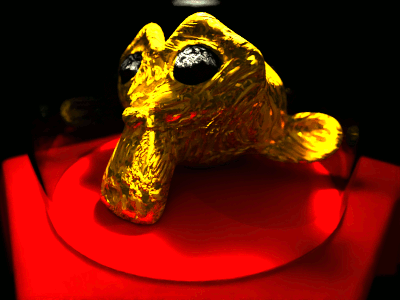
\includegraphics[width=\linewidth]{Medien/suzanne-raw}
				\caption{Raw}
			\end{subfigure}
			\begin{subfigure}{0.33\linewidth}
				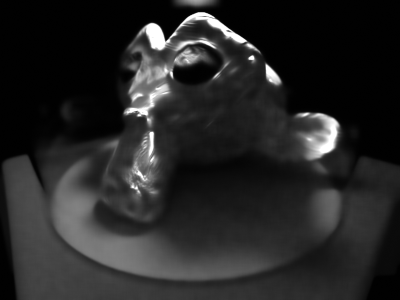
\includegraphics[width=\linewidth]{Medien/suzanne-intensity}
				\caption{Intensität}
			\end{subfigure}
			\begin{subfigure}{0.33\linewidth}
				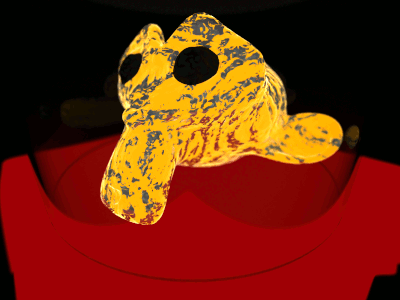
\includegraphics[width=\linewidth]{Medien/suzanne-albedo}
				\caption{Albedo}
			\end{subfigure}
			\begin{subfigure}{0.33\linewidth}
				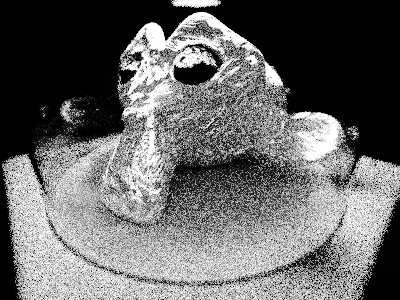
\includegraphics[width=\linewidth]{Medien/suzanne-variance}
				\caption{Varianz}
			\end{subfigure}
			\begin{subfigure}{0.33\linewidth}
				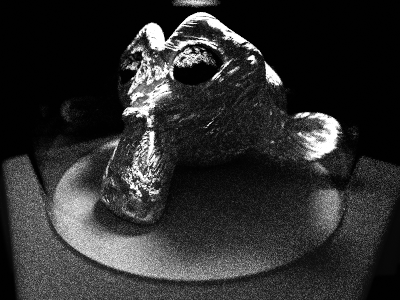
\includegraphics[width=\linewidth]{Medien/suzanne-sw}
				\caption{Schwarz-Weiß}
			\end{subfigure}
			\begin{subfigure}{0.33\linewidth}
				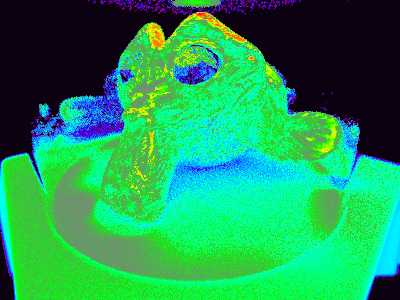
\includegraphics[width=\linewidth]{Medien/suzanne-false-color}
				\caption{Falschfarben}
			\end{subfigure}
			\caption[Suzanne in verschiedenen Renderpasses]{Suzanne, das Maskottchen von Blender mit Goldmaterial in verschiedenen Render-Passes}
			\label{fig:suzanne}
		\end{figure}
		\autoref{fig:suzanne} besteht aus mehreren Teilen, die mit  \lstinline[language=thesis-latexbeispiel]|\begin{subfigure}{0.33\linewidth}| in die \lstinline[language=thesis-latexbeispiel]|figure|-Umgebung aufgenommen werden können. 
		\lstinline[language=thesis-latexbeispiel]|0.33\linewidth| gibt dabei an, dass die Breite der eingefügten Unterabbildung \SI{33}{\percent} der aktuellen Textbreite entsprechen soll.
		
	\section{Tabellen}
		\autoref{tab:beispiel} zeigt eine beispielhafte Tabelle.
		Tabellen werden in der \lstinline[language=thesis-latexbeispiel]|table|-Umgebung gesetzt und sind genau wie Abbildungen \emph{float}-Objekte (siehe \autoref{sec:wissen:float}).
		Die eigentliche Tabelle kann dann \zb{} mit der \lstinline[language=thesis-latexbeispiel]|tabular|-Umgebung gesetzt werden.
		\LaTeX-Editoren wie \emph{TeXstudio} bieten benutzerfreundliche Hilfmittel zur Bearbeitung und automatischen Quelltextformatierung von Tabellen, falls man im Quelltext den Überblick verlieren sollte.
		\begin{table}[bh]
			\centering
			\begin{vorlagenbeispiel}
				\begin{tabular}{l|cr} % lcr: jeder Buchstabe steht für eine Spalte
					(l)eft  & (c)enter & (r)ight \\ % Spalten werden mit & getrennt, Zeilen mit \\ beendet
					\hline                          % \hline erzeugt eine horizontale Linie
					Hier    & steht    & etwas   \\
					in      & einer    & Tabelle
				\end{tabular}
			\end{vorlagenbeispiel}
			\caption{Beispiel zu Tabellen}
			\label{tab:beispiel}
		\end{table}
		\begin{lstlisting}[language=thesis-latexbeispiel]
\begin{table}
	\centering
	\begin{tabular}{l|cr} % lcr: jeder Buchstabe ist eine Spalte
		% Spalten werden mit & getrennt und mit \\ beendet
		(l)eft  & (c)enter & (r)ight \\	
		\hline  % erzeugt eine horizontale Linie
		Hier    & steht    & etwas   \\
		in      & einer    & Tabelle
	\end{tabular}
	\caption{Beispiel zu Tabellen}
	\label{tab:beispiel}
\end{table}
		\end{lstlisting}
		
		
	\section{Quellcode}
		\emph{Für Quellcode nutzt diese Vorlage das Paket \lstinline|listings|.}
		\medskip
		
		Mit \lstinline{\lstinline[language=C]|printf("%d", 42);|} kann Quellcode, z.B. \begin{vorlagenbeispiel}
		\lstinline[language=C]|printf("%d", 42);|
		\end{vorlagenbeispiel} mitten im Text gesetzt werden.
		Der optionale Parameter \lstinline[language=thesis-latexbeispiel]|language=C| gibt dabei an, dass der gezeigte Code in der Programmiersprache \emph{C} vorliegt.
%		
		Die Dokumentation des \lstinline[language=thesis-latexbeispiel]|listings|-Paketes enthält eine vollständige Liste der vordefinierten Programmiersprachen.
		Es gibt ausserdem die Möglichkeit Syntaxhighlighting für weitere Sprachen selber zu definieren.
		\bigskip
		
		Einen abgesetzten Code-Block erzeugt man mit \lstinline[language=thesis-latexbeispiel]|\begin{lstlisting}[language=C]|. Es ist auch möglich Quellcode-Dateien direkt einzubinden (\lstinline[language=thesis-latexbeispiel]|\lstinputlisting{/pfad/zum/quell.code}|), nur einen bestimmten Ausschnitt des Quellcodes anzuzeigen oder die Zeilennummerierung anzupassen (siehe \autoref{code}).
		
		\begin{vorlagenbeispiel}
			\begin{lstlisting}[label=code, language=C, caption={Hello World-Beispiel im lstlisting-Beispiel},firstnumber=1234, emph={printf, schokostuecke}] 
#include <stdio.h>    // Für printf/scanf etc.
#include <stdlib.h>   // Speicherverwaltung & EXIT_SUCCESS/EXIT_FAILURE-Makros

int main(void){
	printf("Hallo LaTeX!\n"); // Textausgabe-Beispiel
	return EXIT_SUCCESS;
}

// In dieser Vorlage sind auch ä,ö,ü,ß und Ä,Ö,Ü erlaubt
			\end{lstlisting}
		\end{vorlagenbeispiel}
		
		Neben \lstinline|language| gibt es noch weitere optionale Parameter, mit denen das Erscheinungsbild angepasst werden kann.
		In \autoref{code} wurden \lstinline|label=labelname| (kann man referenzieren), \lstinline|caption={Beschriftung des Quellcode-Blocks}| und \lstinline|firstnumber=1234| zum Anpassen der Zeilennummerierung verwendet.
	
	\section{Labels \& Referenzen}\label{label-name}
		Überschriften, Abbildungen, Tabellen usw. werden von \LaTeX{} automatisch nummeriert.
%		
		Will man auf einen bestimmten Textabschnitt oder z.B. auf eine Grafik verweisen, so setzt man am Ziel ein \lstinline|\label{labelname}| und referenzenziert dieses dann mit \lstinline|\ref{labelname}|. \lstinline|\autoref{labelname}| ergänzt automatisch den Typ des referenzierten Objekts:
%		
		\begin{vorlagenbeispiel}
		Wenn ich den aktuellen Abschnitt mit \lstinline|ref| referenziere sieht, ergibt sich \ref{label-name} (also nur die Nummer), nutzt man \lstinline|\autoref{labelname}]| ist auch der Typ des Objekts mit dabei: \autoref{label-name}.
%		
		Es ist natürlich auch möglich, \autoref{code} oder \autoref{fig:beispiel} zu referenzieren.
		\end{vorlagenbeispiel}
		
		Mit dem Befehl \lstinline|\nameref{labelname}| erhält man statt der Nummer den Namen des referenzierten Objekts:
		\begin{vorlagenbeispiel}
			Der aktuelle Abschnitt hat die Nummer \ref{label-name} und heißt \enquote{\nameref{label-name}}.
		\end{vorlagenbeispiel}
			
	\section{URLs}
		Mit \lstinline[language=thesis-latexbeispiel]|\url{https://www.blender.org}| lassen sich URLs setzen, die man im PDF dann auch anklicken kann. Der dezente Rahmen um den Link herum wird lediglich angezeigt, beim Drucken aber nicht mit ausgedruckt.
		
		\begin{vorlagenbeispiel}
			Die Open-Source Software Blender (\url{https://www.blender.org}) ist ein mächtiges Allround-Werkzeug für die Erstellung von 3D-Grafik, welches unter anderem die Bereiche Modellierung, Texturierung, Rendering, Rigging, Physik-Simulation, Partikelsimulation, Sculpting, Animation, Videotracking, Videobearbeitung, Compositing und Skripting abdeckt.
		\end{vorlagenbeispiel}
		\medskip

		Will man einen Link absichtlich nur im PDF setzen, die URL aber nicht als Text anzeigen, ist dies mit \lstinline[language=thesis-latexbeispiel]|\href{url}{text}| möglich:
%		
		\begin{vorlagenbeispiel}
			Mit dem sogenannten \href{https://www.blender.org/features/grease-pencil/}{Grease Pencil}-Werkzeug können Künstler 2D Zeichnungen in einer 3D Umgebung erstellen.
			Ursprünglich lediglich ein einfaches Werkzeug für Anmerkungen (daher der Name) wurde es seit \href{https://www.blender.org/download/releases/2-73/}{Blender Version 2.73} zu einem deutlich mächtigeren Werkzeug zur Animation im 2D-Stil weiterentwickelt.
		\end{vorlagenbeispiel}		
		
	\section{Todos}
			Solange die Thesis noch nicht fertig ist, wird man immer mal wieder \enquote{Todos} haben, also Dinge, die noch zu erledigen sind.
			Dank dem \LaTeX-Paket \lstinline[language=thesis-latexbeispiel]|todonotes| kann man diese ganz einfach mit \lstinline[language=thesis-latexbeispiel]|\todo{Hier ist noch etwas zu tun}|\todo{Hier ist noch etwas zu tun} hinzufügen.
	%		
			Mit \lstinline[language=thesis-latexbeispiel]|\listoftodos| lässt sich eine Liste aller Todos im aktuellen Dokument ausgeben.
		
	\section{Glossareinträge \& Symbole}
		\emph{Für Glossareinträge und Symbole nutzt diese Vorlage das Paket \lstinline|glossaries-extra|}
		\medskip
		
		\subsection{Glossar}
			Glossareinträge werden in der Datei \lstinline|Glossar.tex| definiert. Mit \lstinline[language=thesis-latexbeispiel]|\gls{labelname}| können sie im Text verwendet werden:
%			
			\begin{vorlagenbeispiel}
				Es gibt ganz tolle \gls{crc}-Algorithmen, die eine \gls{crc} wirklich genau nach dem Schema typischer \glspl{crc} berechnen.
				Hier ist ein \gls{ex} für einen Glossar-Eintrag. 
				Und hier noch die tolle Abkürzung \gls{svm}, \gls{bspw} stehend für \gls{svm}.
			\end{vorlagenbeispiel}
		\subsection{Symbole}
			Mathematische und physikalische Symbole können ebenfalls in der \lstinline|Glossar.tex| angegeben werden.
			Im Text werden sie mit \lstinline[language=thesis-latexbeispiel]|\glssymbol{labelname}| angesprochen\footnote{Mit \textbackslash gls würde lediglich ihr Name ausgegeben}:
%			
			\begin{vorlagenbeispiel}
				Die ersten drei Buchstaben des griechischen Alphabets sind \glssymbol{alpha}, \glssymbol{beta} und natürlich \glssymbol{gamma}. Die Leere Menge wird mit \glssymbol{emptyset} notiert.
			\end{vorlagenbeispiel}  % Beispiele zu LaTeX
s
	%%%%%%%%%%%%%%%%%%%%%%%%%%%%%%%%%%%%%%%%%%%%%%%%%%%%%%%%%%%%%%%%%%%%%%%%%%%%
	%%%%%%%%%%%%%%%%%%%%%%%%%%%%%%%%%%%%%%%%%%%%%%%%%%%%%%%%%%%%%%%%%%%%%%%%%%%%
	%%% ENDE %%% ENDE %%% ENDE %%% ENDE %%% ENDE %%% ENDE %%% ENDE %%% ENDE %%%%
	%%%%%%%%%%%%%%%%%%%%%%%%%%%%%%%%%%%%%%%%%%%%%%%%%%%%%%%%%%%%%%%%%%%%%%%%%%%%
	%%%%%%%%%%%%%%%%%%%%%%%%%%%%%%%%%%%%%%%%%%%%%%%%%%%%%%%%%%%%%%%%%%%%%%%%%%%%
\end{document} 